% Template for PLoS
% Version 3.4 January 2017
%
% % % % % % % % % % % % % % % % % % % % % %
%
% -- IMPORTANT NOTE
%
% This template contains comments intended 
% to minimize problems and delays during our production 
% process. Please follow the template instructions
% whenever possible.
%
% % % % % % % % % % % % % % % % % % % % % % % 
%
% Once your paper is accepted for publication, 
% PLEASE REMOVE ALL TRACKED CHANGES in this file 
% and leave only the final text of your manuscript. 
% PLOS recommends the use of latexdiff to track changes during review, as this will help to maintain a clean tex file.
% Visit https://www.ctan.org/pkg/latexdiff?lang=en for info or contact us at latex@plos.org.
%
%
% There are no restrictions on package use within the LaTeX files except that 
% no packages listed in the template may be deleted.
%
% Please do not include colors or graphics in the text.
%
% The manuscript LaTeX source should be contained within a single file (do not use \input, \externaldocument, or similar commands).
%
% % % % % % % % % % % % % % % % % % % % % % %
%
% -- FIGURES AND TABLES
%
% Please include tables/figure captions directly after the paragraph where they are first cited in the text.
%
% DO NOT INCLUDE GRAPHICS IN YOUR MANUSCRIPT
% - Figures should be uploaded separately from your manuscript file. 
% - Figures generated using LaTeX should be extracted and removed from the PDF before submission. 
% - Figures containing multiple panels/subfigures must be combined into one image file before submission.
% For figure citations, please use "Fig" instead of "Figure".
% See http://journals.plos.org/plosone/s/figures for PLOS figure guidelines.
%
% Tables should be cell-based and may not contain:
% - spacing/line breaks within cells to alter layout or alignment
% - do not nest tabular environments (no tabular environments within tabular environments)
% - no graphics or colored text (cell background color/shading OK)
% See http://journals.plos.org/plosone/s/tables for table guidelines.
%
% For tables that exceed the width of the text column, use the adjustwidth environment as illustrated in the example table in text below.
%
% % % % % % % % % % % % % % % % % % % % % % % %
%
% -- EQUATIONS, MATH SYMBOLS, SUBSCRIPTS, AND SUPERSCRIPTS
%
% IMPORTANT
% Below are a few tips to help format your equations and other special characters according to our specifications. For more tips to help reduce the possibility of formatting errors during conversion, please see our LaTeX guidelines at http://journals.plos.org/plosone/s/latex
%
% For inline equations, please be sure to include all portions of an equation in the math environment.  For example, x$^2$ is incorrect; this should be formatted as $x^2$ (or $\mathrm{x}^2$ if the romanized font is desired).
%
% Do not include text that is not math in the math environment. For example, CO2 should be written as CO\textsubscript{2} instead of CO$_2$.
%
% Please add line breaks to long display equations when possible in order to fit size of the column. 
%
% For inline equations, please do not include punctuation (commas, etc) within the math environment unless this is part of the equation.
%
% When adding superscript or subscripts outside of brackets/braces, please group using {}.  For example, change "[U(D,E,\gamma)]^2" to "{[U(D,E,\gamma)]}^2". 
%
% Do not use \cal for caligraphic font.  Instead, use \mathcal{}
%
% % % % % % % % % % % % % % % % % % % % % % % % 
%
% Please contact latex@plos.org with any questions.
%
% % % % % % % % % % % % % % % % % % % % % % % %

\documentclass[10pt,letterpaper]{article}
\usepackage[top=0.85in,left=2.75in,footskip=0.75in]{geometry}

%% added PLR
\newif\ifsubmissionversion
%\submissionversionfalse
\submissionversiontrue
\newif\ifincludesupplement
\includesupplementtrue
%\includesupplementfalse
\newif\iffloatsatend
\floatsatendfalse
%\floatsatendtrue
\newif\ifincludefigs
\includefigstrue
%\includefigsfalse
\iffloatsatend
\usepackage[nomarkers]{endfloat}
\fi
%% end added PLR

% amsmath and amssymb packages, useful for mathematical formulas and symbols
\usepackage{amsmath,amssymb}

% Use adjustwidth environment to exceed column width (see example table in text)
\usepackage{changepage}

% Use Unicode characters when possible
\usepackage[utf8x]{inputenc}

% textcomp package and marvosym package for additional characters
\usepackage{textcomp,marvosym}

% cite package, to clean up citations in the main text. Do not remove.
\usepackage{cite}

% Use nameref to cite supporting information files (see Supporting Information section for more info)
\usepackage{nameref}
\usepackage[hidelinks]{hyperref}

% line numbers
\usepackage[right]{lineno}

% ligatures disabled
\usepackage{microtype}
\DisableLigatures[f]{encoding = *, family = * }

% color can be used to apply background shading to table cells only
\usepackage[table]{xcolor}

% array package and thick rules for tables
\usepackage{array}

% create "+" rule type for thick vertical lines
\newcolumntype{+}{!{\vrule width 2pt}}

% create \thickcline for thick horizontal lines of variable length
\newlength\savedwidth
\newcommand\thickcline[1]{%
  \noalign{\global\savedwidth\arrayrulewidth\global\arrayrulewidth 2pt}%
  \cline{#1}%
  \noalign{\vskip\arrayrulewidth}%
  \noalign{\global\arrayrulewidth\savedwidth}%
}

% \thickhline command for thick horizontal lines that span the table
\newcommand\thickhline{\noalign{\global\savedwidth\arrayrulewidth\global\arrayrulewidth 2pt}%
\hline
\noalign{\global\arrayrulewidth\savedwidth}}


% Remove comment for double spacing
%\usepackage{setspace} 
%\doublespacing

% Text layout
\ifsubmissionversion
    \raggedright
    \setlength{\parindent}{0.5cm}
    \textwidth 5.25in 
    \textheight 8.25in
\else
    \usepackage{fullpage}
\fi

% Bold the 'Figure #' in the caption and separate it from the title/caption with a period
% Captions will be left justified
\usepackage[aboveskip=1pt,labelfont=bf,labelsep=period,justification=raggedright,singlelinecheck=off]{caption}
\renewcommand{\figurename}{Fig}

% Use the PLoS provided BiBTeX style
\bibliographystyle{latex/plos2015}

% Remove brackets from numbering in List of References
\makeatletter
\renewcommand{\@biblabel}[1]{\quad#1.}
\makeatother

% Leave date blank
\date{}

% Header and Footer with logo
\usepackage{graphicx}
\ifsubmissionversion
    \usepackage{lastpage,fancyhdr}
    \usepackage{epstopdf}
    \pagestyle{myheadings}
    \pagestyle{fancy}
    \fancyhf{}
    \setlength{\headheight}{27.023pt}
    \lhead{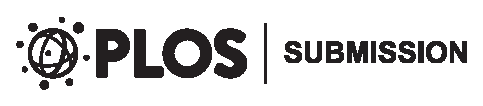
\includegraphics[width=\textwidth]{latex/PLOS-submission.eps}}
    \rfoot{\thepage/\pageref{LastPage}}
    \renewcommand{\footrule}{\hrule height 2pt \vspace{2mm}}
    \fancyheadoffset[L]{2.25in}
    \fancyfootoffset[L]{2.25in}
    \lfoot{\sf PLOS}
\fi

%% Include all macros below

\newcommand{\e}[1]{{\mathbb E}\left[ #1 \right]}
\newcommand{\given}{\mid}
\newcommand{\secref}[1]{``\nameref{#1}''}
\newcommand{\tri}{\textit{trichocarpa}} 
\newcommand{\bals}{\textit{balsamifera}}


\newcommand{\gb}[1]{{\it\color{magenta}{(#1)}}}
\newcommand{\plr}[1]{{\it\color{purple}{(#1)}}}
\newcommand{\gc}[1]{{\it\color{blue}{(#1)}}}


\newcommand{\R}{\mathbb{R}}
\renewcommand{\P}{\mathbb{P}}
\newcommand{\E}{\mathbb{E}}
\newcommand{\var}{\mathop{\mbox{Var}}}
\newcommand{\cov}{\mathop{\mbox{cov}}}
\newcommand{\supp}{\mathop{\mbox{supp}}}
\newcommand{\sgn}{\mathop{\mbox{sgn}}}
\newcommand{\bone}{\mathbf{1}}

%% END MACROS SECTION


\begin{document}
\vspace*{0.2in}

% Title must be 250 characters or less.
\begin{flushleft}
{\Large
\textbf\newline{Inferring continuous and discrete population genetic structure across space}
}
\newline
% Insert author names, affiliations and corresponding author email (do not include titles, positions, or degrees).
\\
Gideon S.\  Bradburd\textsuperscript{1,*},
Graham M.\  Coop\textsuperscript{2,\Yinyang},
Peter L.\  Ralph\textsuperscript{3,\Yinyang},
\\
\bigskip
\textbf{1}
Department of Integrative Biology, 
Ecology, Evolutionary Biology, and Behavior Graduate Group,
Michigan State University, MI 48824
\\
\textbf{2}
Center for Population Biology,
Department of Evolution and Ecology, 
University of California, Davis, CA 95616
\\
\textbf{3} 
Institute of Ecology and Evolution,
Departments of Mathematics and Biology,
University of Oregon, Eugene, OR 97403
\\
\bigskip
\textbf{*}bradburd@msu.edu

\bigskip

%
% Primary Equal Contribution Note
\Yinyang These authors contributed equally to this work.

\end{flushleft}
% Please keep the abstract below 300 words
\section*{Abstract}

A classic problem in population genetics is the characterization 
of discrete population structure in the presence of 
continuous patterns of genetic differentiation.
Especially when sampling is discontinuous, 
the use of clustering or assignment methods may incorrectly ascribe
differentiation due to continuous processes (e.g., geographic isolation by distance)
to discrete processes, such as geographic, ecological, or reproductive barriers 
between populations.
This reflects a shortcoming of current methods for inferring and 
visualizing population structure when applied to genetic data
deriving from geographically distributed populations.
Here, we present a statistical framework for the simultaneous inference 
of continuous and discrete patterns of population structure.
The method estimates ancestry proportions for each 
sample from a set of two-dimensional population layers, 
and, within each layer, estimates a rate at which relatedness decays with distance.
This thereby explicitly addresses the ``clines versus clusters" problem in 
modeling population genetic variation,
and ameliorates the overfitting that nonspatial models are prone to.
The method produces useful descriptions of structure in genetic relatedness
in situations where separated, geographically distributed populations interact,
as after a range expansion or secondary contact.
We demonstrate the utility of this approach using simulations 
and by applying it to empirical datasets of poplars and black bears in North America.

\ifsubmissionversion
\newpage
\fi


% Please keep the Author Summary between 150 and 200 words
% Use first person. PLOS ONE authors please skip this step. 
% Author Summary not valid for PLOS ONE submissions.   
\section*{Author summary}
One of the first steps in the analysis of genetic data, 
and a principal mission of biology, 
is to describe and categorize natural variation. 
A continuous pattern of differentiation (isolation by distance), 
where individuals found closer together in space 
are, on average, more genetically similar than individuals sampled farther apart, 
can confound attempts to categorize natural variation into groups.  
This is because current statistical methods for assigning individuals to discrete clusters 
cannot accommodate spatial patterns, 
and so are forced to use clusters to describe what is in fact
continuous variation. 
As isolation by distance is common in nature, 
this is a substantial shortcoming of existing methods.
In this study, we introduce a new statistical method 
for categorizing natural genetic variation - 
one that describes variation as a combination of continuous and discrete patterns.
We demonstrate that this method works well and can capture patterns in
population genomic data without resorting to splitting populations
where they can be described by continuous patterns of variation.

%Using simulated data, we show how current approaches can be misleading, 
%and also demonstrate that our new method works well.  
%We predict that our method will be an important tool for the analysis of genetic data.

\ifsubmissionversion
\linenumbers
\fi

\newpage
\section*{Introduction}
A fundamental quandary in the description of biological diversity is
the fact that diversity shows both discrete and continuous patterns. 
For example, reasonable people can disagree about whether two 
populations are separate species because the 
process of speciation is usually gradual, and so there is no set point
in the continuous divergence of populations when they unambiguously become discrete species.
The issue of identifying meaningful biological subunits 
extends below the species level, as patterns of phenotypic
and genetic diversity within and among populations are shaped
by continuous migration and drift, as well as by more discrete events, 
such as rapid expansions, bottlenecks, rare long-distance migration,
and separation by geographic barriers.
Both discrete and continuous components
are required to accurately describe most species' patterns of genetic relatedness.

From a practical standpoint, even while acknowledging continuous
processes, we often need to identify somewhat separable populations 
from which individuals are sampled \cite{wright1949genetical}.
Delineating populations is useful for systematics and for
informing conservation priorities \cite{Moritz1994,Waples_1998,Moritz_etal_2002}.
Furthermore, we often need to identify subsets of indivduals resulting from reasonably coherent
evolutionary histories for downstream analyses to learn about population history and adaptation.
Conversely,
the substantial information available from continuous, geographic differentiation
(e.g., adaptation along a climatic gradient)
can be confounded by discrete historical processes (e.g., admixture),
requiring methods that can disentangle the two.

There have been many methods proposed to characterize population
genetic structure,
including generating population phylogenies \cite{CavalliSforza1975, treemix},
dimensionality-reduction approaches, 
such as principal components analysis 
\cite{meirmans2009genodive,menozzi1978synthetic,novembre_interpreting_2008, price2006eigenstrat},
and model-based clustering approaches 
(e.g., \cite{STRUCTURE, falush2003, hubisz2009,ADMIXTURE, 
FINESTRUCTURE, fastStructure, huelsenbeck2007inference, 
Corander2003,TESS,geneland}), among others.
Each of these methods perform best in particular situations,
but many can give misleading results when applied to data 
that show a continuous pattern of differentiation,
as that produced by geographic isolation by distance 
\cite{Wright1943, novembre_interpreting_2008, Frantz2009}.
Here, we will focus on model-based clustering, the most widely used class of approaches for population delineation.
Existing model-based clustering methods model each individual's genotypes 
as random draws from a set of underlying, unobserved population clusters, 
each with a characteristic set of allele frequencies, which are estimated. 
These underlying frequencies are identical 
for all individuals assigned to a cluster, 
\emph{regardless} of their spatial location. 
Spatial information has been incorporated into some of these methods, 
by, for example, placing spatial priors on ancestry proportions \cite{geneland,TESS}, 
but this does not address the underlying issue that 
these methods assume that allele frequencies 
are constant in a cluster across the species' range.  

\emph{Isolation by distance} (IBD) refers to a pattern of increasing genetic differentiation
with geographic separation,
which occurs when geographically restricted dispersal allows
genetic drift to build up differentiation between distant locations
\cite{Wright1943}. 
Theoretical work,
mostly derived from ``stepping-stone'' models 
\cite{kimura1964stepping,sawyer1976stepping,shiga1984stepping},
gives us some analytical predictions for isolation by distance
\cite{malecot1969mathematics,Slatkin1985,epperson2003geographical}, 
but substantial work remains to be done \cite{barton2002neutral,barton2013modelling}.
% Isolation by distance has been modeled in both spatially continuous frameworks 
% in which an individual's parents are found within some radius of that individual's location,
% and discrete, ``stepping-stone'' frameworks \cite{kimura1964stepping},
% in which migration occurs only between neighboring demes.
Given the generality of the circumstances that generate a pattern of isolation by distance, 
it is unsurprising that isolation by distance is very widespread in nature \cite{meirmans2012,Sexton_etal_2014}.

The ubiquity of isolation by distance presents a challenge for models of discrete population structure,
as it is frequently difficult to determine whether observed patterns of genetic variation are 
continuously distributed across a landscape, or instead are partitioned in discrete clusters.
This problem can be compounded if sampling is done unevenly or discretely across a population or species' range,
and has given rise to a debate in the population genetic literature
about how best to describe sets of individuals using continuous clines and discrete clusters 
(e.g., \cite{SerrePaabo2004,rosenberg2005clines}).

Existing model-based clustering approaches can only describe continuous patterns of variation using
discrete clusters, and so tend to erroneously describe continuously distributed variation with multiple clusters that 
show spatially autocorrelated cluster membership \cite{Frantz2009,meirmans2012}.
In analyses of empirical datasets, which often show strong isolation by distance,
model-based clustering approaches will therefore tend to overestimate
the number of discrete clusters present. 

To address this, we set out to develop
a model-based clustering method that, when possible, uses isolation by distance 
to explain observed genetic variation.
With an explicit spatial component, discrete population structure need only be invoked when genetic differentiation 
in the data deviates significantly from that expected given geographic separation.
In this paper, 
% we present a statistical method for simultaneously 
% modeling continuous and discrete patterns of population structure.
we model genetic variation in genotyped individuals as 
partitioned within or admixed across a specified number of discrete layers,
within each of which relatedness decays as a parametric function of the distance between samples.
We also implement a cross-validation approach for comparing and selecting models across different numbers of layers,
and we demonstrate the utility of our approach using both simulated and empirical data.
The implementation of this method, \texttt{conStruct} (for ``\emph{con}tinuous \emph{struct}ure"), 
is available as an R package at 
\href{https://github.com/gbradburd/conStruct}{https://github.com/gbradburd/conStruct}.


% \section*{Methods}
\section*{Results}

\paragraph{Data}
The statistical framework of our approach is conceptually similar to that in \cite{Wasser2004}, \cite{BEDASSLE}, and \cite{spacemix},
although we use a somewhat different summary statistic than in this previous work.
The model works with allele frequencies at $L$ unlinked, bi-allelic single nucleotide polymorphisms (SNPs) genotyped across $N$ samples.
Each ``sample'' may be a single individual,  
a collection of individuals from a location, 
or frequencies estimated from pooled sequencing.
From these we compute the \emph{allelic covariance} 
between samples $i$ and $j$, denoted $\widehat{\Omega}_{i,j}$,
as the expected covariance of distinct individual alleles 
chosen from each of the two samples at a random locus.
More precisely, suppose that we pick a random bi-allelic locus uniformly,
pick a random ``reference'' allelic state from the two seen at that locus,
and, in each sample, draw one random allele,
recording $X_i = 1$ if the allele drawn in sample $i$ matches the random reference,
and $X_i = 0$ otherwise.
Then, 
\begin{equation} \label{eqn:first_allelic_cov}
    \widehat{\Omega}_{i,j} = \cov[X_i, X_j] .
\end{equation}
Each $X_i$ behaves marginally as a fair coin --
in particular, $\P\{X_i = 1\} = 1/2$, so $\widehat{\Omega}_{i,i} = 1/4$ for every $i$ --
all information enters through \emph{correlations}.


Although we describe this as a covariance between individually drawn alleles,
$\widehat{\Omega}_{i,j}$ is in fact also the covariance between the allele frequencies
of a randomly chosen allele in samples $i$ and $j$, as long as $i \neq j$.
The choice of allele does not affect subsequent calculations, and so may be arbitrary, 
and $\widehat \Omega$ can be calculated as 
(derived in \secref{allelic_cov}):
\begin{equation}
\widehat{\Omega}_{i,j} = 
    \frac{1}{L} \sum_{\ell=1}^L (f_{i,\ell}-1/2) (f_{j,\ell}-1/2) \qquad \text{for } i \neq j.
\label{allelic_covariance}
\end{equation}
This definition of covariance differs from the usual ``genetic covariance'' \cite{mcvean_genealogical_2009}
in that (a) we do not subtract locus means,
and so to make the statistic insensitive to choice of reference allele, 
(b) we randomly choose a reference allele at each locus.
As noted in \cite{EEMS}, for $i \neq j$,
this can also be calculated as $\Omega_{i,j} = (1 - 2 \pi_{i,j})/4$,
where $\pi_{i,j}$ is the genetic distance,
i.e., mean density of sites at which random samples from $i$ and $j$ differ.

\paragraph{Continuous and discrete differentiation}
Clustering approaches to describing genetic variation
are useful because population history can often be meaningfully described on a coarse scale
by interactions between discrete ``populations''
whose relationships are delimited by patterns of glaciation,
large-scale migration,
mountain ranges, and the like.
Here we add a spatial component within each such discrete historical component,
which we refer to as a set of ``layers'' that overlay the modern map.
We imagine each layer as a geographically distributed population 
that extends over the entire sampled range of the populations. 
As depicted in Figure \ref{schematic},
each sample is composed of a mixture of contributions from each of these layers,
with the relative contributions of each layer described by
a set of ``admixture proportions'' (the $w_i^{(k)}$).
These layers thus take the place of ``clusters'' in clustering methods,
but we do not adopt this term, 
as ``spatial cluster'' suggests a clustering in space, 
while our layers may contribute to genetic variation 
across the entire geographic range.

%they connote a lack of geographical separation within each.

Within each of these layers,
allele frequencies have positive covariance at geographically close locations,
but this covariance is allowed to decay as geographic distance increases.
This pattern of spatial decay reflects how migration between neighboring demes  
homogenizes allele frequency changes that arise locally due to drift, 
but less effectively homogenizes geographic distant demes,
resulting in a continuous pattern of isolation by distance within each layer.
There is a fixed amount of covariance between layers, irrespective of spatial location.
Within each layer, allele frequencies are expected to change gradually with distance,
but observed frequencies can change abruptly at many loci 
if the proportions of ancestry individuals derive from each layer 
(the ``admixture'' proportions) 
do so as well. 

To allow flexibility in the form of the decay of allelic covariance with geographic distance within each layer, 
we define the covariance within layer $k$ between samples $i$ and $j$ to be:
\begin{equation}
G^{(k)}_{i,j} 
    = 
    \alpha^{(k)}_0 \left( \text{exp} \left( -(\alpha^{(k)}_D D_{i,j}) ^ {\alpha^{(k)}_2}	\right) \right) + \phi^{(k)}
\label{within_layer_covariance}
\end{equation}
where the superscript $(k)$ denotes parameters specific to the $k$th layer.
The quantity $D_{i,j}$ is the observed geographic distance between samples $i$ and $j$,
and the $\alpha^{(k)}$ parameters control the shape of the decay of
covariance with distance in the layer.
Our choice of a powered-exponential decay, 
as parameterized by the $\alpha$s, 
is a flexible and standard choice in spatial statistics \cite{Diggle1998}, 
and is not chosen to match a particular population genetics model. 
% (Analytical theory \cite{barton2002neutral} predicts the decay should be proportional to $\exp{-D}/\sqrt{D}$.)
The $\phi^{(k)}$ is a parameter that describes the background covariance within the layer. 
If two samples draw 100\% of their ancestry from layer $k$, then their covariance under the model is $G^{(k)}_{i,j}$;
if they are furthermore geographically very close ($D_{i,j}=0$)
they will have covariance $\alpha^{(k)}_0 +  \phi^{(k)}$.
If the geographic distance between them is very large, 
their covariance will be equal to the background level $\phi^{(k)}$ within the layer.
The ``shared drift'' parameter $\phi^{(k)}$ is analogous to 
the branch length connecting the $k$th population to the population ancestral to all modeled
layers (see for example \cite{patterson_ancient_2012,peter_fstats}),
although they cannot be directly compared because 
we are modeling the allelic, rather than genetic, covariance. 
In \secref{rationale} we lay out a
simple model of allele frequencies underlying this covariance model.

We then allow samples to draw their ancestry from more than one layer.
The ``admixture'' proportion of the $i$th sample in the $k$th layer, denoted $w^{(k)}_i$,
gives the genome-wide proportion of alleles from sample $i$ that derive from
layer 
$k$ (and so $\sum_{k=1}^K w^{(k)}_i =1$).
A visual representation of the method is shown in Fig \ref{schematic}.

\begin{figure}
	\centering
	\ifincludefigs
		{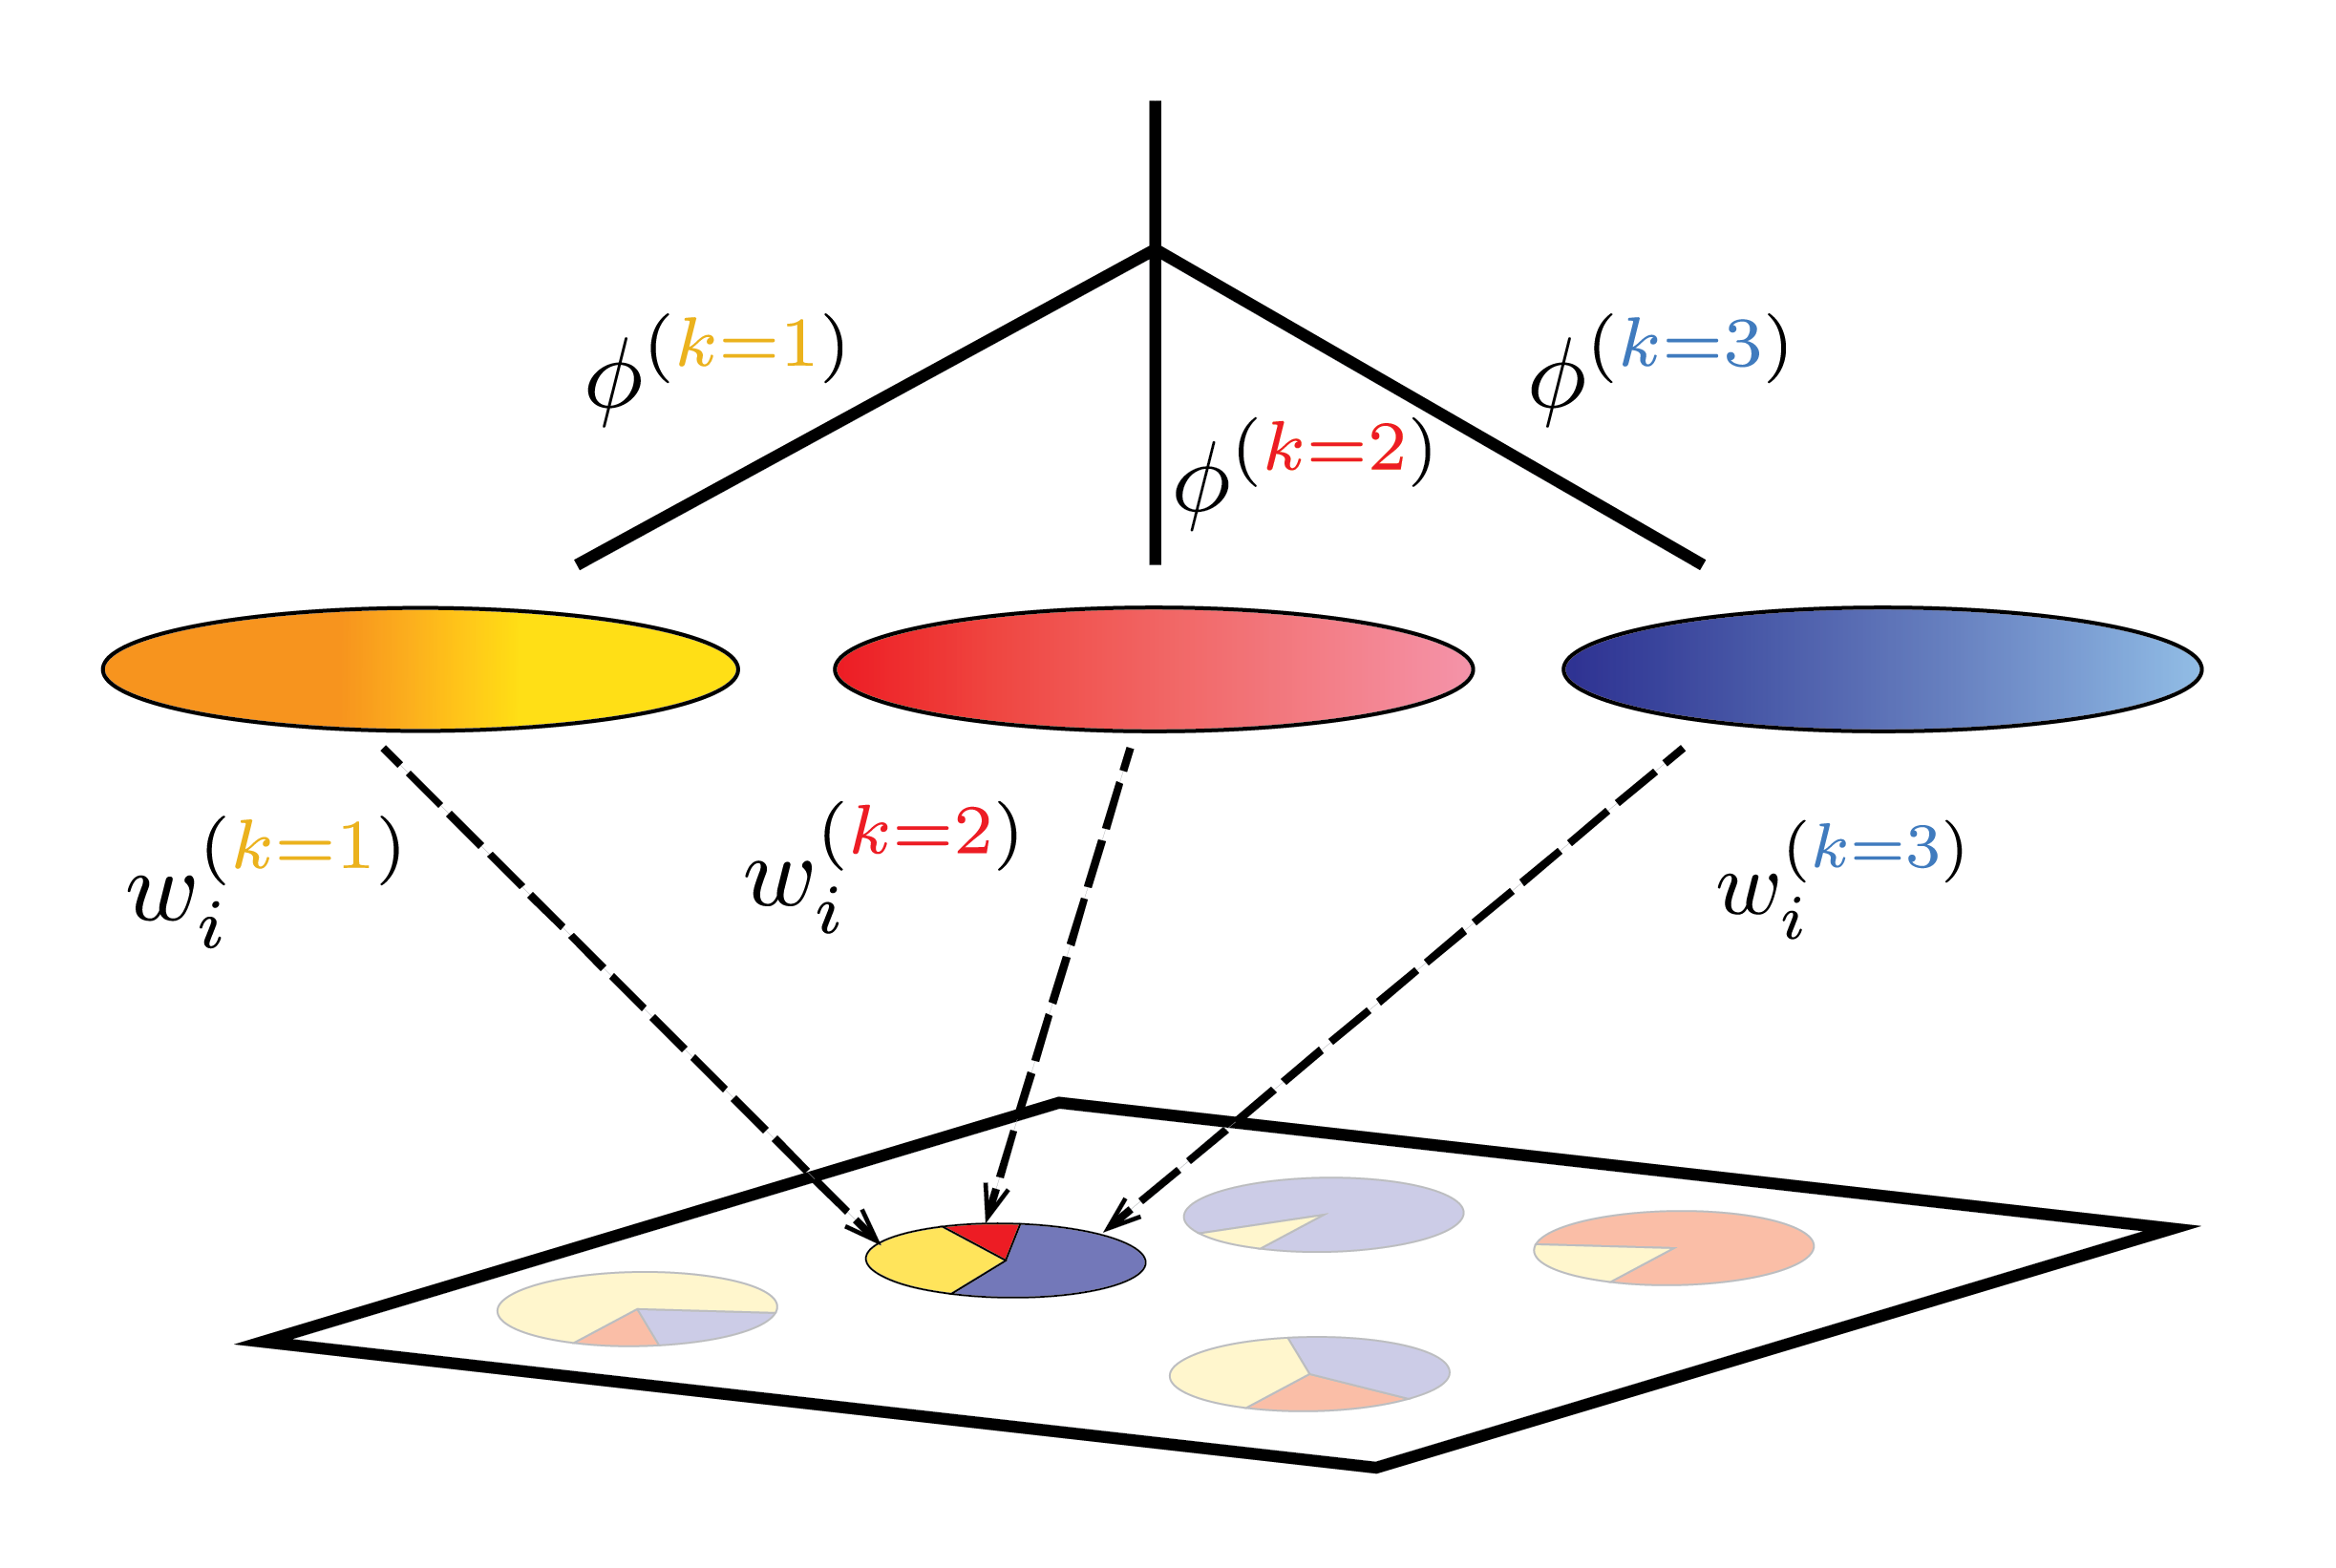
\includegraphics[width=\textwidth]{figs/schematic/method_schematic.png}}
	\fi	
		\caption{Schematic of our method, using $K=3$ as an example.
                 Spatial autocorrelation of allele frequencies within each layer is depicted by color gradients, 
			     and $\phi^{(k)}$ denotes the covariance shared by samples with ancestry entirely in the $k$th layer.
			     Sampled populations on the landscape are inferred to be admixed between these layers; 
			     the $i$th sample draws proportion $w^{(k)}_i$ of its ancestry from layer $k$.
			     For convenience, each layer is depicted as a small square, but in fact, 
			     each layer exists everywhere in the sampled area,
			     so the small dashed circles on each layer show where 
			     the location of the highlighted admixed sample intersects each layer.
			    }\label{schematic}
\end{figure}

We can then describe the covariance between samples $i$ and $j$ across all $K$ layers, $\Omega_{i,j}$,
by summing their within-layer spatial covariances ($G_{i,j}^{(k)}$ in layer $k$),
weighted by the relevant admixture proportions.
\begin{equation}
    \Omega_{i,j} = \gamma + \sum_{k=1}^K w^{(k)}_i w^{(k)}_j
G^{(k)}_{i,j} + \delta_{i,j}\eta_i .
\label{cross_layer_covariance}
\end{equation}
In this equation, $w^{(k)}_i w^{(k)}_j$ is the proportion of alleles that \emph{both}
sample $i$ and sample $j$ have inherited from layer $k$.

In addition to the admixture-weighted sum of the within-layer spatial covariances,
this function contains two terms, $\gamma$ and $\delta_{i,j}\eta_i$.
The first, $\gamma$, describes the global allelic covariance between all samples, 
and arises because all samples share an ancestral mean allele frequency at each locus,
which generates a base-line covariance.
In the final term, $\delta_{i,j}$ is an indicator variable that takes a value of 1 when $i$ equals $j$ and 0 otherwise,
and $\eta_i$ adds variance specific to sample $i$.
This term on the diagonal of the parametric covariance matrix captures processes shaping variance within the sampled deme, 
such as inbreeding and the sampling process.

\paragraph{Likelihood and inference}
If the allele frequency deviations at each locus
were independent between loci and multivariate normally distributed across populations, 
their allelic covariance $\widehat{\Omega}$ 
would be Wishart distributed with degrees of freedom equal to $L$, 
the number of loci genotyped.
We use this as a convenient approximation to the true distribution described above,
and so define the likelihood of the allelic covariance to be
\begin{equation}
    P(\widehat{\Omega} \; | \; \Omega) 
    = 
    \mathcal{W} \left( L\widehat{\Omega} \; | \; \Omega,L\right) ,
\end{equation}
where $\mathcal{W}$ is the Wishart likelihood function.
Statistical nonindependence between loci (linkage disequilibrium)
will decrease the effective
number of degrees of freedom.  
One possible solution, which we have not yet found necessary to implement,
would be to estimate an \emph{effective} number of loci 
by introducing a parameter to modify the given degrees of freedom 
and thereby informally model linkage between loci (e.g., \cite{EEMS}).

We estimate the values of the parameters of the model using a Bayesian approach.
Acknowledging the dependence of the parametric covariance matrix $\Omega$ on its constituent parameters
$w,\alpha,\phi,\eta,\gamma$ and on the (observed) geographic distances $D$ 
with the notation $\Omega(w,\alpha,\phi,\eta,\gamma,D)$,
we denote the posterior probability density of the parameters as:
\begin{equation}
P\left( w,\alpha,\phi,\eta,\gamma \;|\; \widehat{\Omega} \right) 
    \propto
    P\left(\widehat{\Omega} \; | \; \Omega(w,\alpha,\phi,\eta,\gamma,D) \right)
    P(w)P(\alpha)P(\phi)P(\eta)P(\gamma) ,
\end{equation}
where $P(w)$, $P(\alpha)$, $P(\phi)$, $P(\eta)$, and $P(\gamma)$, are prior distributions.
All parameters are given (half-)Gaussian priors 
except for $\alpha_2$, which is uniform on $(0,2)$, 
and $w$, for which we use an independent Dirichlet of dimension $K$ for each sample
(see Table \ref{tab:param_prior_tab} for specifics).
Parameters are independent between layers.
We use Hamiltonian Monte Carlo as implemented in STAN \cite{stan, NUTS, stan_lib, rstan} 
to estimate the posterior distribution on the parameters.
Our R package, \texttt{conStruct} (for ``\emph{con}tinuous \emph{struct}ure"),
functions as a wrapper around this inference machinery.


\paragraph{Relationship of this model to nonspatial structure models}

A nice feature of our approach is that the model described in Eq.\ \eqref{cross_layer_covariance} 
contains a nonspatial assignment model as a special case 
(see \secref{model_app} for a more in-depth discussion). 
By setting $\alpha_0^{(k)}$ to zero for all $k$, 
we obtain a nonspatial model in which each cluster has its own allele frequency at each SNP, 
and individuals draw a proportion of their ancestry from each cluster. 
This model is very similar to that of STRUCTURE \cite{STRUCTURE} 
and related models (e.g., \cite{ADMIXTURE}); 
the main difference is that our likelihood assumes that allele frequencies are normally distributed 
around their expectations, 
while the standard assignment methods assume that the error is binomially distributed \cite{Engelhardt2012}.  
(We make this approximation for the substantial advantages in
computational speed.)
The second small difference is that, in the original STRUCTURE model, 
allele frequencies at each locus are independently drawn for each 
cluster \cite{STRUCTURE}, while in conStruct's non-spatial model, 
it is more natural to envision each cluster's allele frequency 
as being drifted away from a single, global allele frequency. 
This makes our model more
closely related to the ``$F$-model'' prior for allele frequencies of \cite{falush2003}.
As these differences are relatively small, we can compare the fit of the different models 
--- spatial vs. nonspatial, across different values of $K$ --- 
by comparing their performance in a common framework. 
We also validate our claim that the results of our nonspatial method 
are a close match to those of STRUCTURE-based approaches.

\paragraph{Choice of layer number and cross-validation}
There are a number of reasons 
why there is no true (or right) number of layers for real datasets,
discussed further in the Discussion.
However, it is still important to assess whether additional layers (larger $K$)
meaningfully model patterns in the data
or merely explain spurious variation introduced by noise
-- in other words, whether additional model complexity
provides significant explanatory power.
Toward that end, we have implemented a method for 
statistically comparing \texttt{conStruct} results across different values of $K$ 
and between the spatial and nonspatial models.

Several approaches have been used as model choice criteria 
for the number of discrete clusters in population genetic data, including: 
comparisons of the likelihood of the data across different values of $K$,
with various criteria on how to choose a single value (e.g., \cite{Evanno2005}),
or with information theoretic penalizations such as AIC or BIC (e.g., \cite{ADMIXTURE});
or comparisons of the marginal likelihood, 
generated either via various approximations (e.g., \cite{STRUCTURE})
or via a more rigorous and computationally intensive approach such as thermodynamic integration \cite{verity_nichols2016}
or inference using a Dirichlet process prior \cite{huelsenbeck2007inference}.
See \cite{verity_nichols2016} for a discussion of these approaches and comparison
between several methods.

We use cross-validation (similar in spirit to \cite{ADMIXTURE_xval}) to attack this problem.
To do this,
we use a ``training" partition of the data (in practice, a random 90\% subset of the loci)
to estimate the posterior distribution of the parameters,
and then calculate the log-likelihood of the remaining ``testing'' loci,
averaged over the posterior.
Prediction accuracy of a particular model (e.g., value of $K$)
is then measured using this log-likelihood,
averaged over a number of independent data partitions.
The best model is judged to be the simplest one with significantly better predictive accuracy
than others (see \secref{Xvalidation} for more on our cross-validation procedure).
In general, larger values of $K$ allow the model more flexibility,
and thus increases the likelihood of the training partition, 
but this improvement in the likelihood will plateau (or even peak), 
as above a certain $K$ the model only fits noise specific to the training data 
rather than generalizable patterns.
At any value of $K$, support for the spatial model over the nonspatial model 
means that isolation by distance is likely a feature of the data.

Cross-validation provides a valuable summary of how much explanatory power
is added by spatial structure within each layer, and each additional layer.
However, we remind users that ``statistical significance does not imply real-world significance','
and so small but statistically significant differences between models
should probably not be relied on too strongly.

Another way to describe the practical significance of additional layers
is to calculate each layer's relative contribution to total covariance, 
and to choose a value of $K$ where all layers have a contribution above some cutoff (e.g. 0.1\%).
The Dirichlet prior on admixture proportions
is quite harsh against intermediate admixture values (see Table \ref{tab:param_prior_tab}),  
encouraging the model to ``not use" unnecessary layers if they are
present in the model, 
so that they will have a low contribution to overall covariance.

To calculate layer contributions, we use the following alternative description of our covariance model:
the genomes of any pair of individuals \emph{agree} with some
background probability at a locus,
but this probability of agreement is increased on any segment of genome 
that both have inherited from the same layer 
(the amount it increases depends on how far apart they are
geographically and on the decay of isolation by distance).
We use this characterization to quantify the relative contributions of each layer,
by computing the average contribution to increased probability of agreement
as described in \secref{layer_contribution}). 
This layer contribution is similar to the ``ancestry contribution'' proposed by \cite{fastStructure}. 
However, each of our layers can induce a different amount of covariance between samples embedded in them, 
so we take that into account when calculating each layer's contribution to the whole.


% \section*{Results}

\subsection*{Simulations}

To test the method, we first generated data using the coalescent simulator \texttt{ms} \cite{Hudson2002}.
In each simulation,
we split a single ancestral population into $K$ subpopulations $\tau_{\text{s}}$ units of coalescent time in the past,
and at time $\tau_{\text{e}}$ in the past,
each of these discrete populations instantaneously colonized a
separate $6 \times 6$ square lattice of demes.
Migration on each lattice was to nearest neighbors (eight neighbors, including diagonals).
Finally, at time $\tau_{\text{a}}$ in the past, 
we collapsed those $K$ discrete layers into a single grid of demes,
choosing various amounts of admixture from these different layers
(see Fig \ref{sim_setup}). 
We collapsed the layers together using random, spatially autocorrelated admixture proportions 
(see \secref{sim_details}).
% so that both the frequencies in layers and the layer memberships are spatially autocorrelated. 
We simulated datasets using $K=1$, 2, and 3 layers;
in each simulation we sampled 10,000 unlinked loci from each of 20 haploid individuals from every deme.
We then ran both spatial and nonspatial \texttt{conStruct} analyses on each simulated dataset with $K$ between 1 and 7,
and compared predictive performance of the models using cross-validation.
% To confirm that results from our nonspatial model were qualitatively similar to those of 
% other nonspatial model-based clustering algorithms, 
For comparison,
we also analyzed each simulated dataset using ADMIXTURE \cite{ADMIXTURE} with $K$ between 1 and 7, 
and compared models using ADMIXTURE's cross-validation procedure with 50 data ``fold" subsets.

With these simulations,
spatial \texttt{conStruct} does not create spurious discrete groupings when there are none:
Figures \ref{simK1_pies}, \ref{simK2_sp_pies}, and \ref{simK3_sp_pies} 
show that subsequent layers beyond the number used for simulation are unused.
When data are simulated with $K=1$ but analyzed with $K>1$, 
the layers are present, but contribute very little to any population.
Even when the spatial model is run with $K=7$, 
the inferred admixture proportions are nearly identical to 
those estimated under the true value of $K$ for each simulation.
Moreover, the method infers the true admixture proportions with high accuracy, tight precision, and good coverage 
(Figs \ref{simK2_adprop_fit} and \ref{simK3_adprop_fit}).

In contrast, the nonspatial model describes geographic variation
using gradients of admixture between more and more discrete clusters
to better approximate the continuous, spatial patterns of relatedness
(depicted in Figs \ref{simK1_pies} and \ref{simK1_nsp_pies}).
% as $K$ in the model increases, 
% the sampled area is increasingly divvied up between clusters 
% with ``centers of mass" in the $K$ geographical extremes of the simulated space.
% At $K=2$, the clusters are centered in opposite corners on the map; 
% at $K=3$, in the lower two corners and the top half; 
% at $K=4$, all four corners, and so on.
The ADMIXTURE results are qualitatively similar, as shown in Figs \ref{admix_simK1}-\ref{admix_simK3}.
Each nonspatial cluster is genetically more similar within itself
than it is to other clusters,
but we know that these boundaries are arbitrary,
because the data were simulated without them.

The spatial model's better fit is reflected by increased predictive accuracy:
as shown in Fig \ref{sim_xvals},
across all models and choices of $K$, the spatial model is correctly preferred over the nonspatial model.
As desired, predictive accuracy of the spatial model increases until the true value of $K$,
and then plateaus or declines
(Figs \ref{sim_xvals}, \ref{simK1_xval}, \ref{simK2_xval}, and \ref{simK3_xval}),
while predictive accuracy of the nonspatial model increases as subsequent clusters are added.
The same holds true for the ADMIXTURE cross-validation results,
in which models that have the largest number of clusters are preferred over all other models,
as shown in Fig \ref{sim_admix_CVerrors}.
% In contrast, the predictive accuracy of the spatial \texttt{conStruct} model
% either plateaus at or declines from the true value of $K$ used to simulate the data 
% (Figs \ref{sim_xvals}, \ref{simK1_xval}, \ref{simK2_xval}, and \ref{simK3_xval}).

The unimportance of spurious layers can be seen in plots of layer contributions
(Figs \ref{simK1_laycon}, \ref{simK2_laycon}, and \ref{simK3_laycon}).
In the spatial analyses, once we pass the true $K$, 
subsequent layers add little in terms of (co)variance explained; 
in contrast, additional clusters in the nonspatial analyses continue to contribute substantially.

\begin{figure}
	\centering
	\ifincludefigs
		{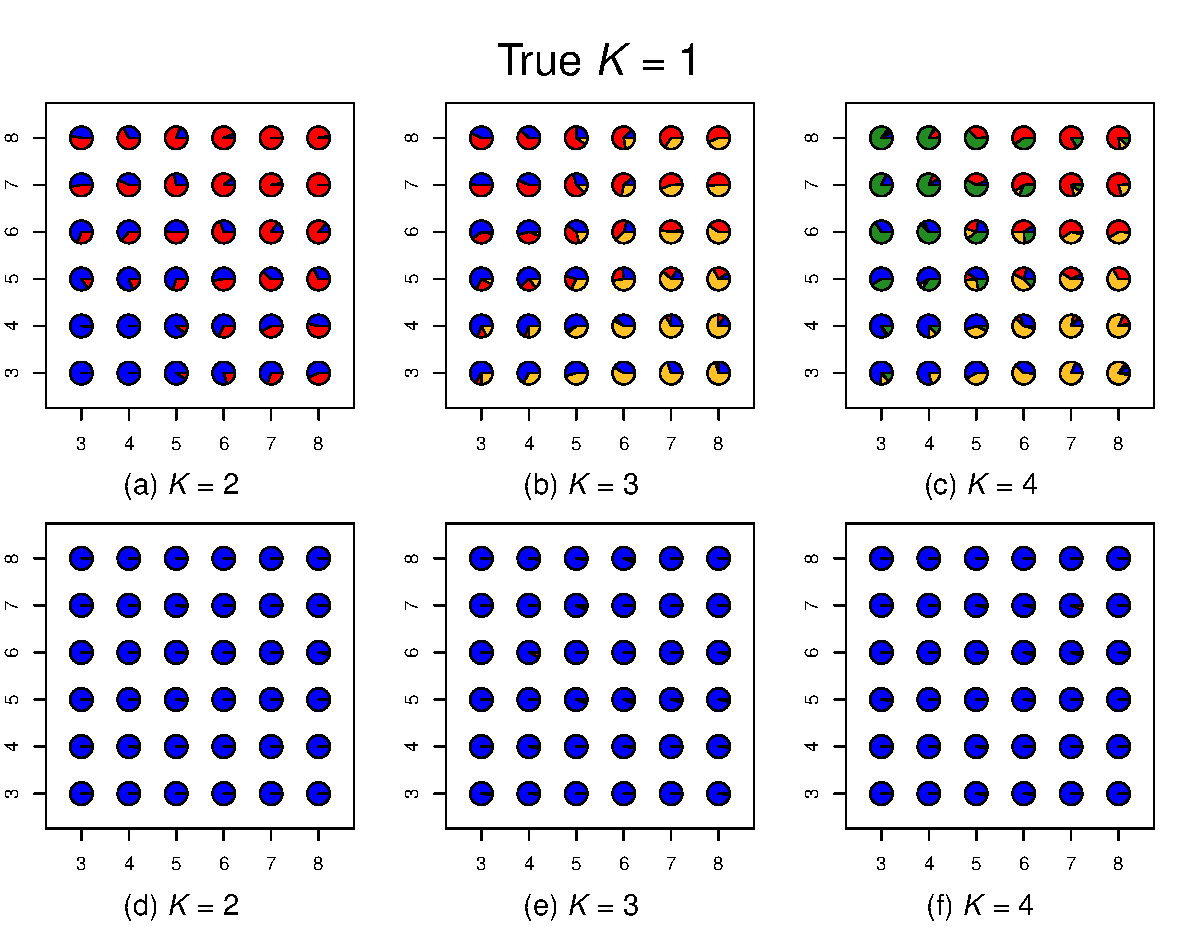
\includegraphics[width=\textwidth]{figs/sims/Fig2_simK1_sp_vs_nsp.pdf}}
	\fi
	\caption{
        Results for data simulated using $K=1$,
	showing maps of admixture proportions estimated using the nonspatial model for $K=2$ through 4 (top row)
	and the spatial model for $K=2$ through 4 (bottom row).
	% The data were simulated using a single layer with nearest-neighbor symmetric migration between demes.
    Since there is only a single layer in the simulation, the spatial model accurately depicts the data
    in all cases, while the nonspatial model creates spurious clusters.
    }\label{simK1_pies}
\end{figure}

\begin{figure}
	\centering
	\ifincludefigs
		{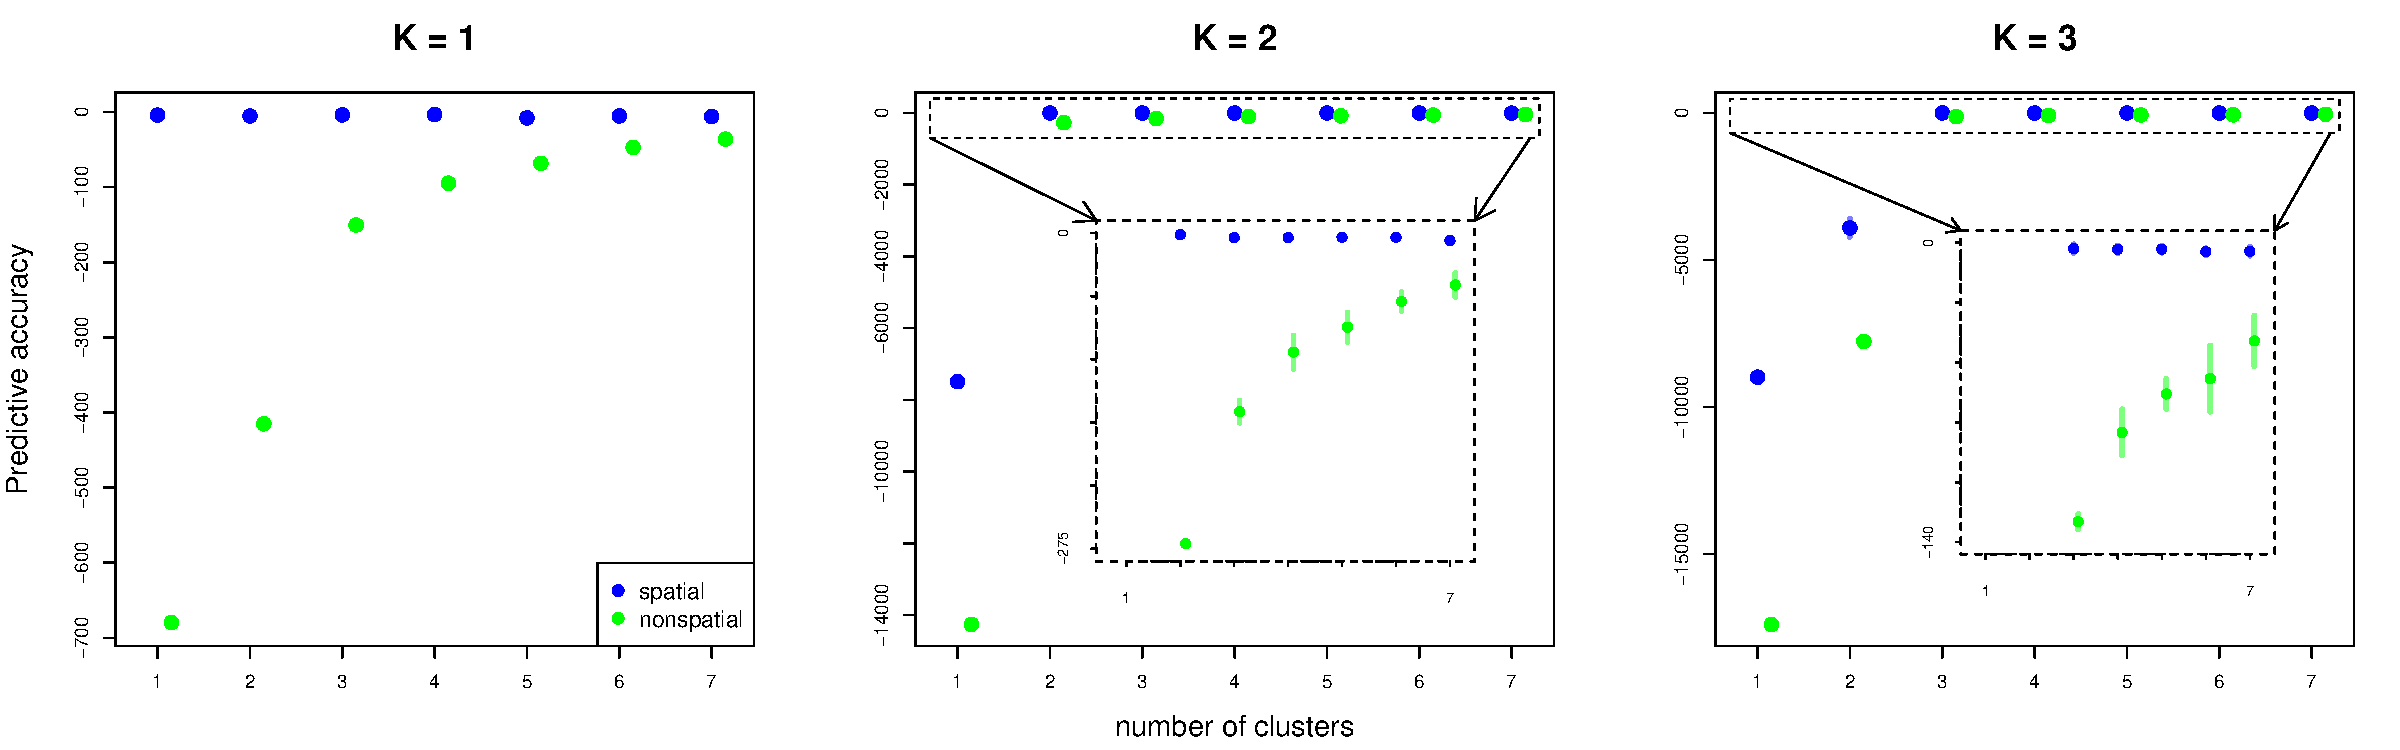
\includegraphics[width=\textwidth]{figs/sims/sim_xvals.pdf}}
	\fi
	\caption{
	Cross-validation results for data simulated under $K=1$, $K=2$, and $K=3$, 
	comparing the spatial and nonspatial \texttt{conStruct} models 
	(in blue and green, respectively) run with $K=1$ through 7.  
	The inset plots zoom in on cross-validation results outlined in the dotted boxes.
    The spatial model shows better model fit at every value of $K$.
    }\label{sim_xvals}
\end{figure}

\begin{figure}
	\centering
	\ifincludefigs
		{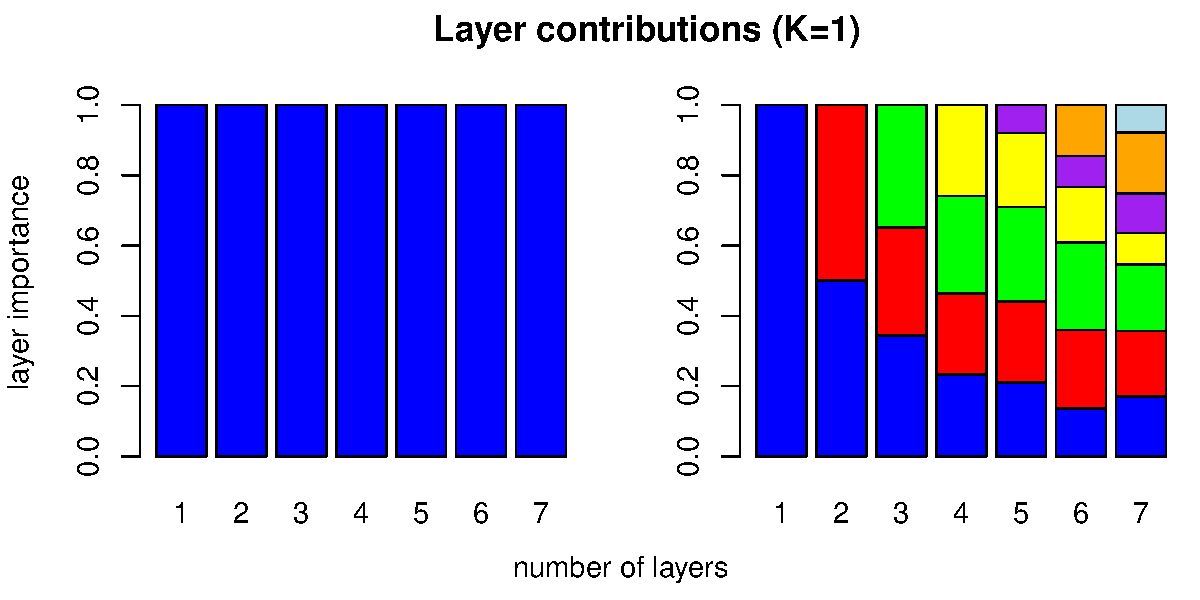
\includegraphics[width=\textwidth]{figs/sims/simK1_laycon_barplots.pdf}}
	\fi
		\caption{
            Results for data simulated using $K=1$, showing
            layer/cluster contributions (i.e., how much each layer/cluster contributes to total covariance),
            from \texttt{conStruct} runs using $K = 1$ through 7 
			for the spatial model (left), and the nonspatial model (right).
			In each run of the nonspatial model, a single layer explained nearly all the covariance
            (additional bars are present but not visible).
		}\label{simK1_laycon}
\end{figure}


\subsection*{Empirical Applications}

To further demonstrate the utility of this method, 
we also applied \texttt{conStruct} to empirical population genomic data from two systems:
a contact zone between two poplar species in northwestern North America,
and a large North American sample of black bears.

\subsubsection*{Poplars}

Trees in the genus \textit{Populus} (poplars, aspens, and cottonwoods) 
are distributed throughout the Northern Hemisphere;
species in the genus regularly co-occur and, 
where they do, they frequently hybridize \cite{eckenwalder1984, Cronk2005}.

\textit{Populus trichocarpa}, the black cottonwood,
and \textit{Populus balsamifera}, the balsam poplar,
have a broad zone of overlap in the Pacific Northwest,
where they are hypothesized to hybridize \cite{geraldes_etal_2014, suarezgonzalez_etal_2016}.
Both species are sampled over a large geographic region, 
and show spatial patterns of genetic and phenotypic variation \cite{slavov_etal_2012, mckown_etal_2013},
making the system well-suited for application of our method.
% to test an analysis designed to describe
% how genetic structure is partitioned both discretely across populations (or species)
% and continuously with geographic distance.
We organize the results of our analyses around the following questions: 
\begin{enumerate}

    \item To what degree has hybridization blurred the boundaries between 
        \textit{trichocarpa} and \textit{balsamifera}?
        (As an extreme case, does genetic differentiation support these as separate species,
        as opposed to a single cline of ancestry?)
    % Given the known history of hybridization between this pair of poplar species, 
    % is there support for two discrete populations, 
    % rather than a single cline of ancestry across their overlap zone?

    \item Does the only significant boundary of population structure
        fall along the species boundary (if any),
        % If there is evidence for discrete population structuring, 
        % does it fall solely along species boundaries, 
        or is there sub-structuring within species?

    \item Does the strength of isolation by distance differ between inferred layers?
        This may indicate, e.g., different speeds of postglacial expansion
        or primary modes of dispersal.
        % Is there support for a pattern of isolation by distance within
        % the inferred layers, and, if so, 
        % does it differ between different layers?

\end{enumerate}

We use data from \cite{geraldes_etal_2014}, 
consisting of 434 individuals sampled from 35 drainages 
genotyped at just over 33,000 loci (map of the sampling shown in Fig \ref{populus_map}).
The number of individuals per drainage ranged between 1 and 50, 
with most sampling concentrated on \tri{} drainages.
The data were generated using an Infinium 34K array designed for \tri{} \cite{geraldes_2013}, 
and showed a strong pattern of bias in allelic dropout 
(the majority of missing data were from drainages with only \textit{Populus balsamifera} individuals).
To ameliorate some of the problems that arise when there is a strong bias in which data are missing, 
we dropped loci for which any data were missing, 
resulting in just over 20,200 loci retained for analysis.  
We then analyzed these data, grouped by drainage, 
using both the spatial and nonspatial \texttt{conStruct} models with $K = 1$ through 7,
and compared these models using cross-validation.
The results of all these analyses are shown in 
Figs \ref{populus_pies} and \ref{populus_xvals}, 
as well as Figs \ref{populus_sp_pies} - \ref{populus_laycon} in the Supplementary Materials.
For comparison, we also ran ADMIXTURE \cite{ADMIXTURE} 
with $K = 1$ through 7, using 50-fold cross-validation to compare model performance
(Figs \ref{populus_admixture} and \ref{poplar_admix_CVerrors}). 

\begin{figure}
	\centering
	\ifincludefigs
		{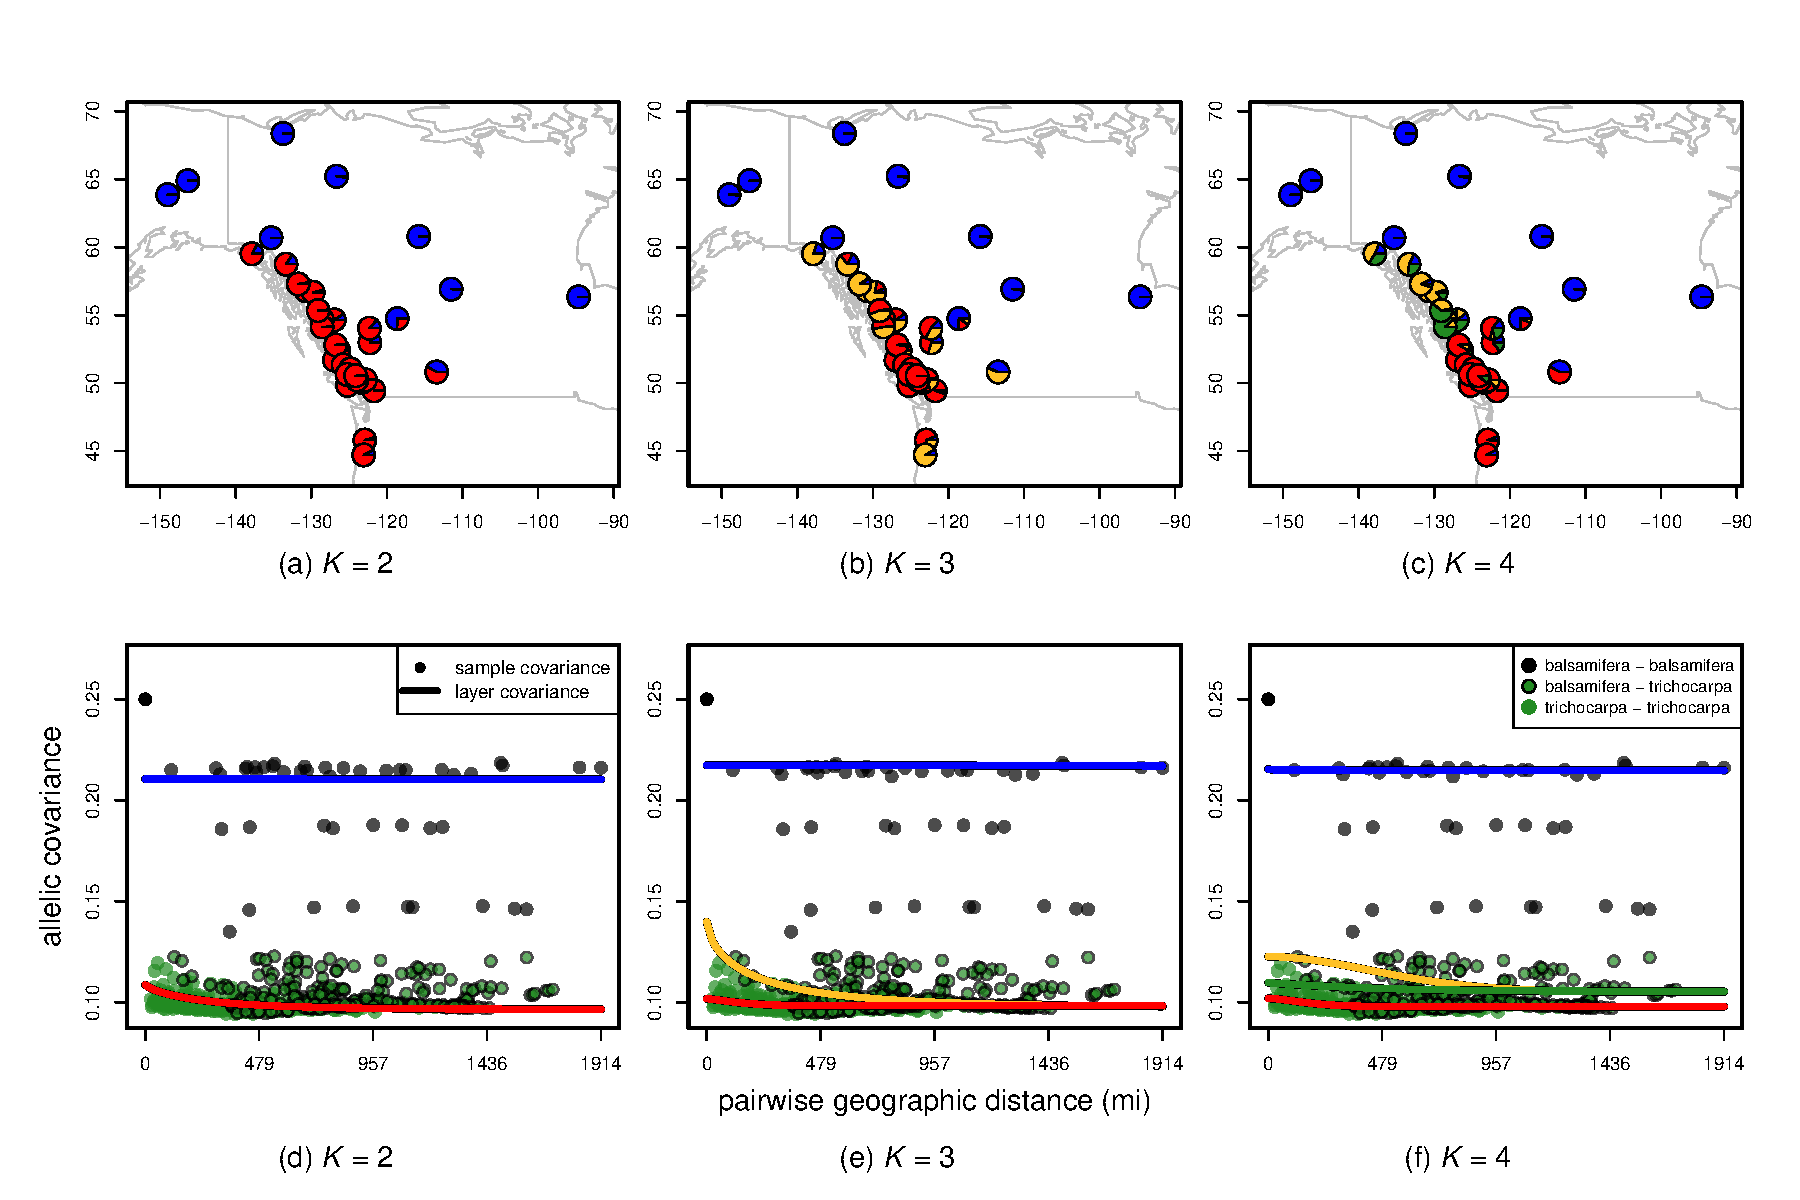
\includegraphics[width=\textwidth]{figs/populus/pop_sp_results.pdf}}
	\fi
	\caption{
	Maps of admixture proportions estimated for the \textit{Populus} dataset 
	using the spatial model for $K=2$ through 4 (a-c), 
	as well as the corresponding layer-specific covariance curves estimated under each model (d-f).
    }\label{populus_pies}
\end{figure}

\begin{figure}
	\centering
	\ifincludefigs
		{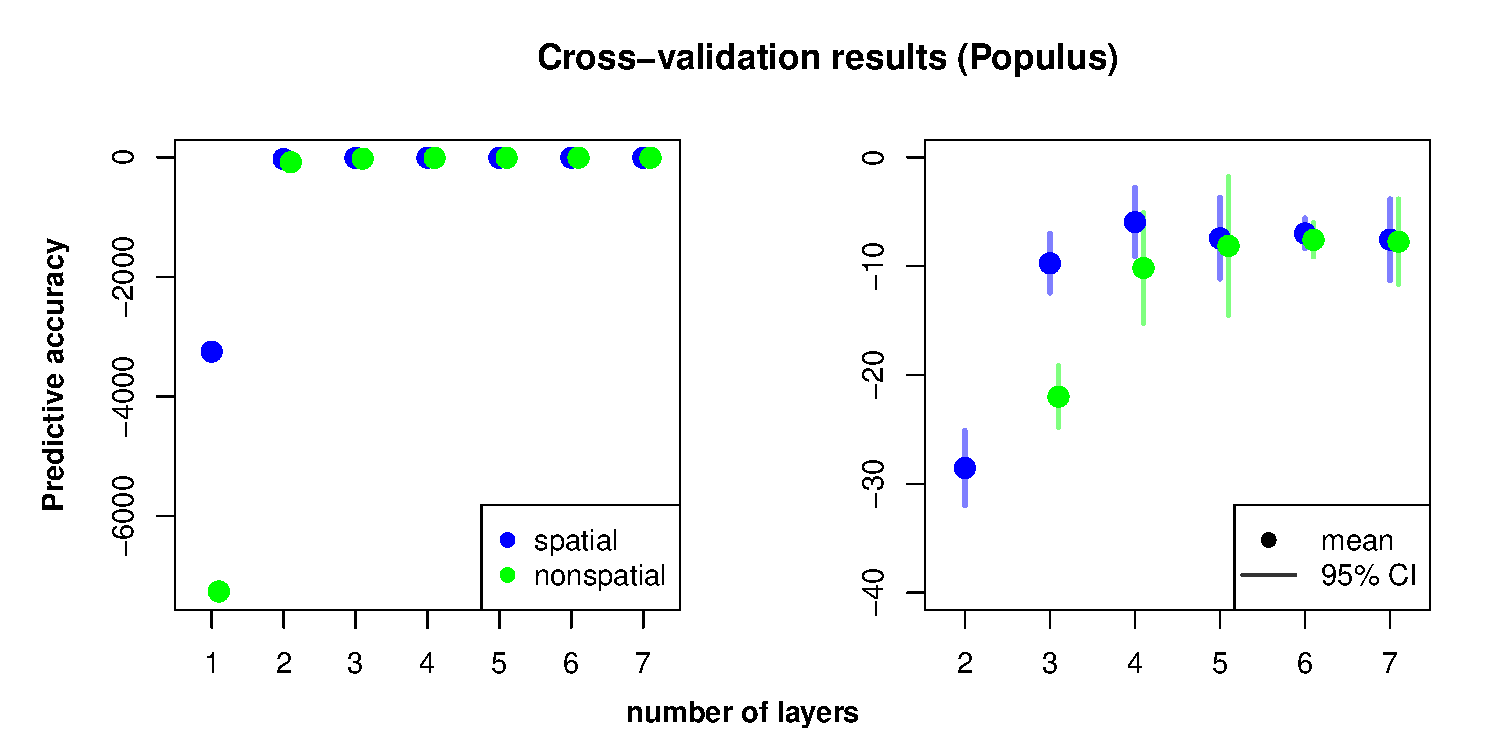
\includegraphics[width=\textwidth]{figs/populus/populus_std_xval.pdf}}
	\fi
	\caption{
	Cross-validation results for \textit{Populus} dataset 
	comparing the spatial and nonspatial \texttt{conStruct} models run with $K=1$ through 7.  
	The first panel in each row shows all results; 
	the second panel zooms in on the results from analyses run with $K = 2$ through 7.
    }\label{populus_xvals}
\end{figure}

All models with $K>1$ assigned the majority of each of the two species
to distinct layers, with some populations drawing ancestry from multiple layers.
Based on cross-validation results, we view the $K=3$ spatial model 
as a sufficient description of the data,
with additional structure of uncertain significance.
This provides strong support for discrete population structure between the two species,
with some admixture,
rather than a single, continuous cline of ancestry.
At all values of $K>1$, discrete population structure was mostly partitioned along species lines; 
at values of $K$ above 2, further discrete substructure was inferred within the \textit{P. trichocarpa} samples,
with no substructure within \bals{}.
There was also strong support for isolation by distance in the dataset, 
but most of this signal seems to derive from the \textit{P. trichocarpa} samples:
% covariance within predominantly \tri{} layers decays more quickly with distance than within the majority \bals{} layer, 
as seen in Figs \ref{populus_pies}d-f and \ref{populus_sp_layer_covs},
there is almost no isolation by distance within the \bals{} layer ($\alpha_D \approx 0$).
Both points are
in agreement with \cite{keller_etal_2010}, 
who found low diversity within the region's \bals{},
probably as the result of a recent postglacial expansion.

A consistent split between layers within \tri{} fell along the ``no-cottonwood belt," 
a region along the central coast of British Columbia in which black
cottonwood is absent (the break between yellow and red, for $K \geq 3$). 
The no-cottonwood belt is hypothesized to divide the species' distribution
into northern and southern groups, which, in a provenance test, 
were experimentally shown to display differences in ecologically relevant phenotypes 
(e.g., pathogen resistance, \cite{xie2009,xie2012}).  
At higher values of $K$, drainages at the southern tip of \tri{} sampling 
begin to split out into their own layers,
perhaps due to introgression from the southern neighbors
\textit{P. angustifolia} or \textit{fremontii} \cite{Zhou2012,geraldes_etal_2014}


Both nonspatial \texttt{conStruct} and ADMIXTURE displayed 
the successive partitioning of space and the clines of admixture seen in the simulation results.
The details of each were somewhat different 
(Fig \ref{populus_nsp_pies} vs. Fig \ref{populus_admixture}), 
and also differed across the replicate analyses, 
but each strongly favored the most cluster-rich model
(Figs \ref{populus_xvals} and \ref{poplar_admix_CVerrors}).

\subsubsection*{Black bears}

The American black bear, \textit{Ursus americanus}, is endemic to North America
and has a broad distribution across the continent.
During the last glacial maximum, 
black bears were confined to isolated glacial refugia, 
from which they subsequently expanded to occupy their current range
\cite{WoodingWard1997,Byun1997,Stone2000,Puckett2015},
%The retreat of the glaciers was relatively recent in units of 
%black bear generation times \cite{Onorato2004}, 
%so we might reasonably expect the divergence accrued between refugia 
%to be reflected in discrete genetic structure between extant populations.
%Black bears are strong dispersers \cite{Moore2014}, 
%but they are distributed across most of the continent, 
%so we may therefore expect them to experience distance-limited 
%mating opportunities and exhibit a pattern of isolation by distance.
likely leading to both continuous and discrete patterns of genetic structure.
We organize our results around the following questions:
\begin{enumerate}
    \item How many distinct populations
        are reflected in modern patterns of genetic variation?
    \item How strong is isolation by distance within each inferred group?
\end{enumerate}
Distinct populations likely represent different glacial refugia,
and differing strengths of isolation by distance might indicate 
different levels of habitat connectivity,
dispersal behavior,
or different postglacial histories.

We use data from \cite{Puckett2015}, consisting of 95 individuals 
sampled across the United States and on the West coast of Canada,
genotyped at just under 22,000 bi-allelic loci.
The distribution of missing data across these individuals was uneven, 
with a few individuals representing most of the missing data, 
so we removed individuals with greater than 4\% missing data, 
resulting in a final dataset of 78 individuals.
We then analyzed these data, treating individuals as the unit of analysis, 
using both the spatial and nonspatial \texttt{conStruct} models with a $K$ of between 1 and 7, 
and compared these models using cross-validation.
We also ran ADMIXTURE \cite{ADMIXTURE} on the same dataset, 
using $K = 1$ through 7, and comparing models using 
ADMIXTURE's cross-validation procedure with 50 data ``fold" subsets.
The results of these analyses are shown in Figs \ref{bear_K3} - \ref{bear_laycon}, 
as well as in Figs \ref{bear_sp_pies} - \ref{bear_admix_CVerrors} in the Supplementary Materials.

\begin{figure}
	\centering
	\ifincludefigs
		{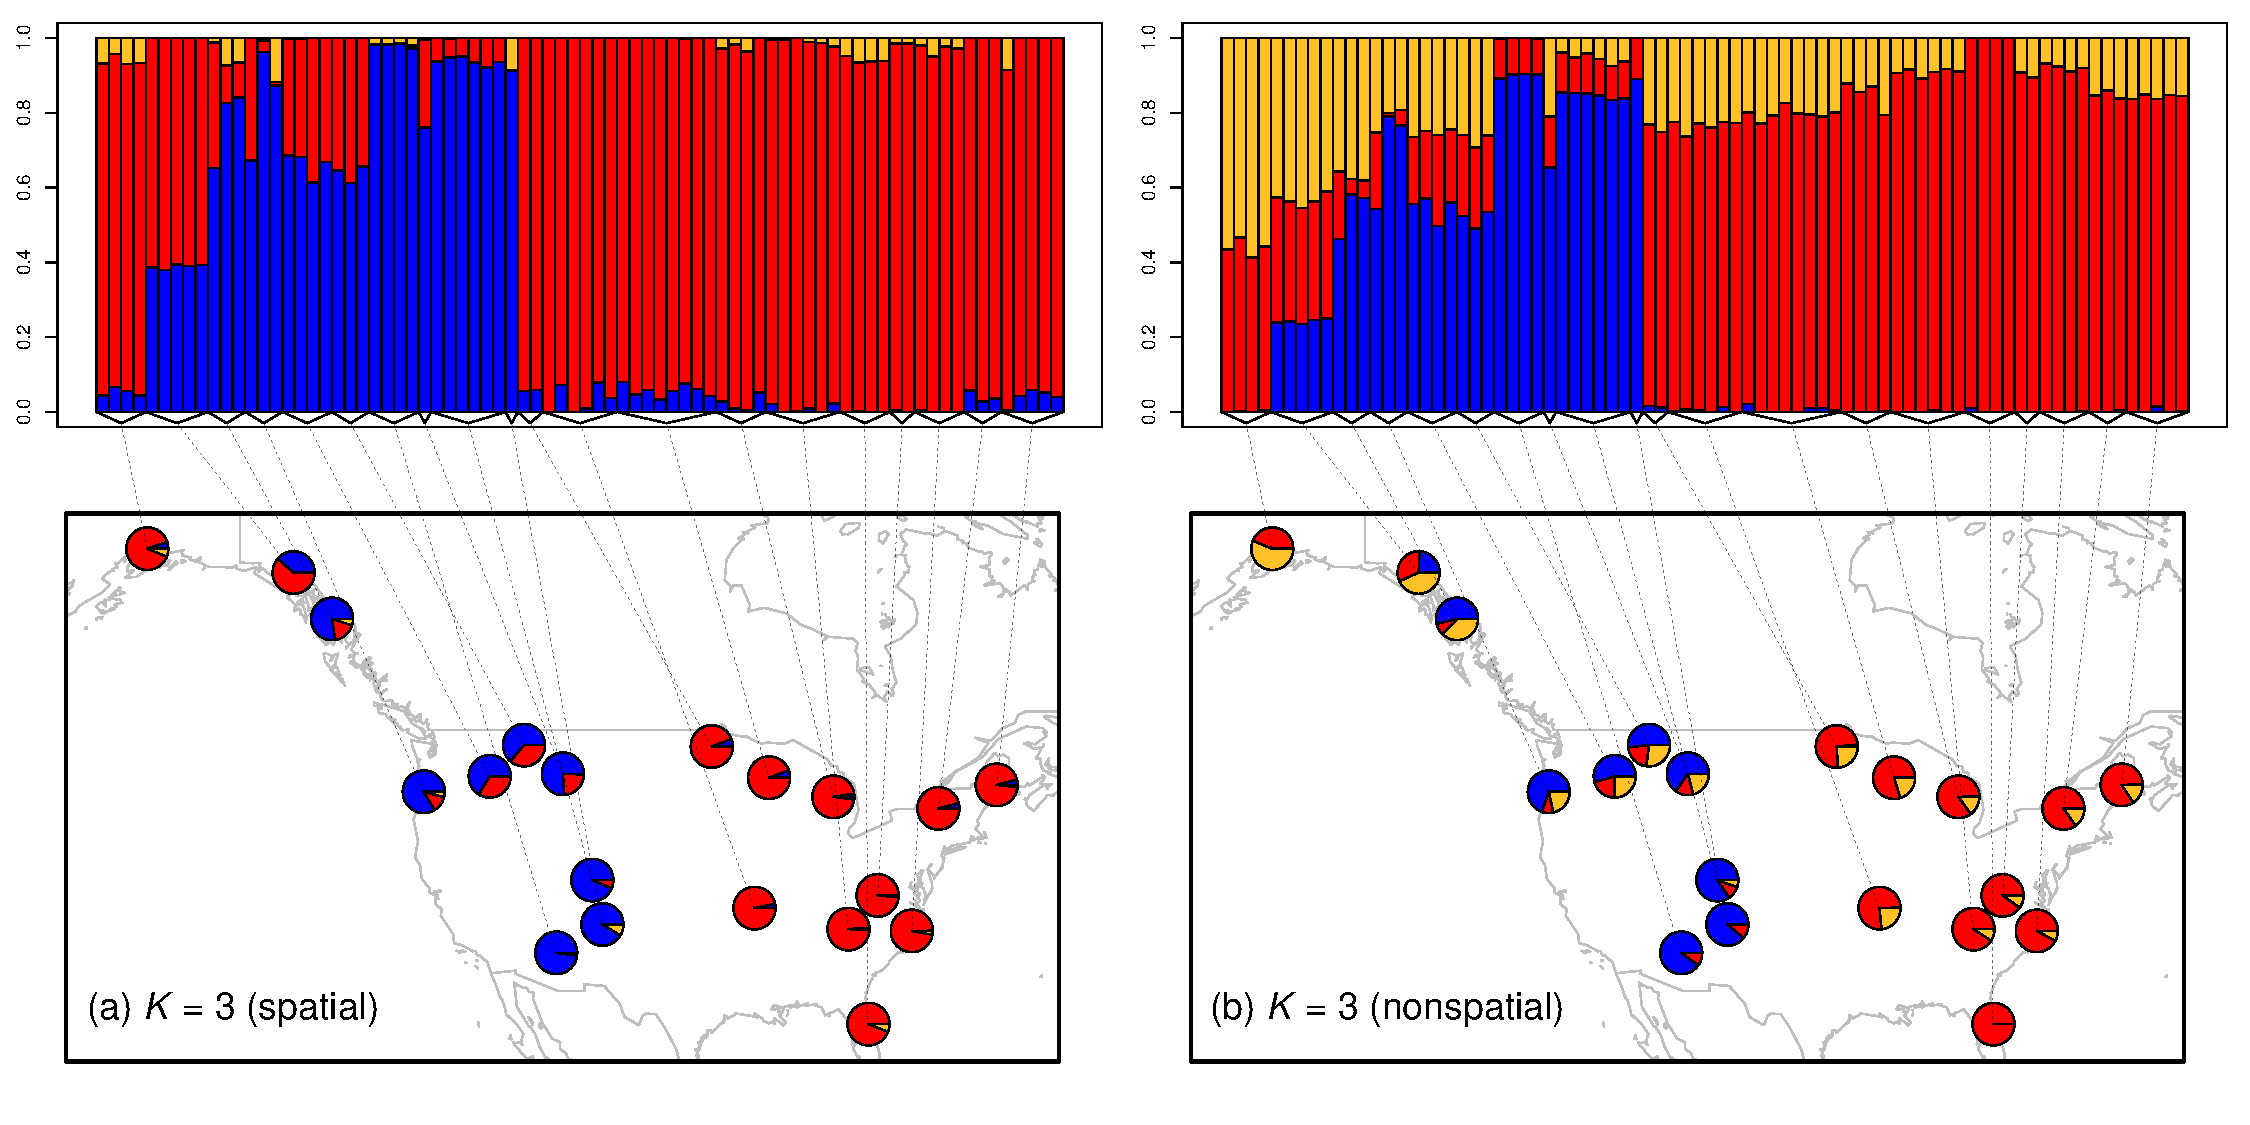
\includegraphics[width=\textwidth]{figs/bears/bears_sp_vs_nsp.pdf}}
	\fi
	\caption{
	Maps of admixture proportions estimated for the black bear dataset 
	using the spatial model (left) and the nonspatial model (right) for $K=3$.
	Pies show mean admixture results across individuals within their diameter, 
	and the admixture results for all individuals included within each group are 
	shown in the plot above.
    }\label{bear_K3}
\end{figure}

\begin{figure}
	\centering
	\ifincludefigs
		{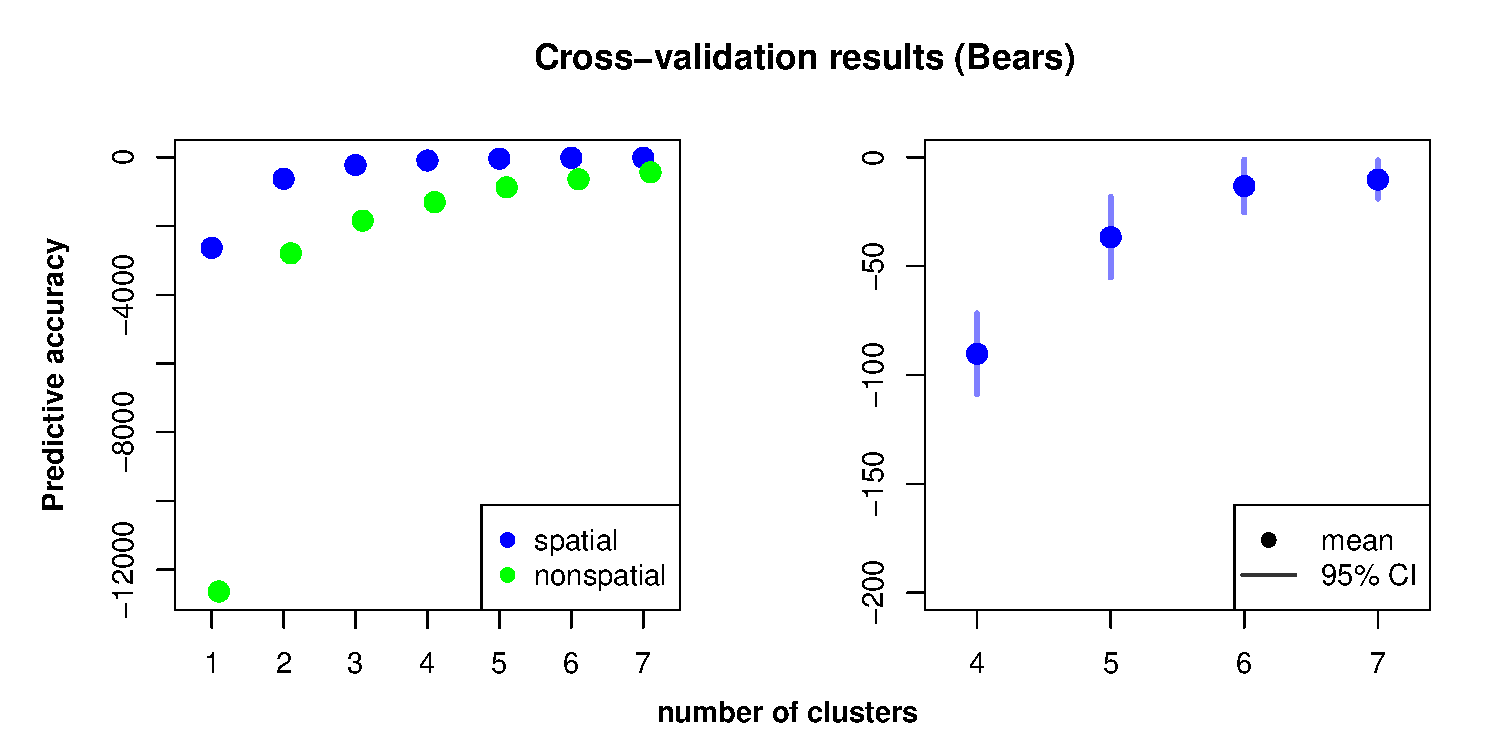
\includegraphics[width=\textwidth]{figs/bears/bear_std_xval.pdf}}
	\fi
	\caption{
	Cross-validation results for the black bear dataset,
	comparing spatial and nonspatial \texttt{conStruct} models run with $K=1$ through 7.  
	The first panel in each row shows all results; 
	the second panel zooms in on the results from the spatial analyses run with $K = 4$ through 7.
    }\label{bear_xvals}
\end{figure}

\begin{figure}
	\centering
	\ifincludefigs
		{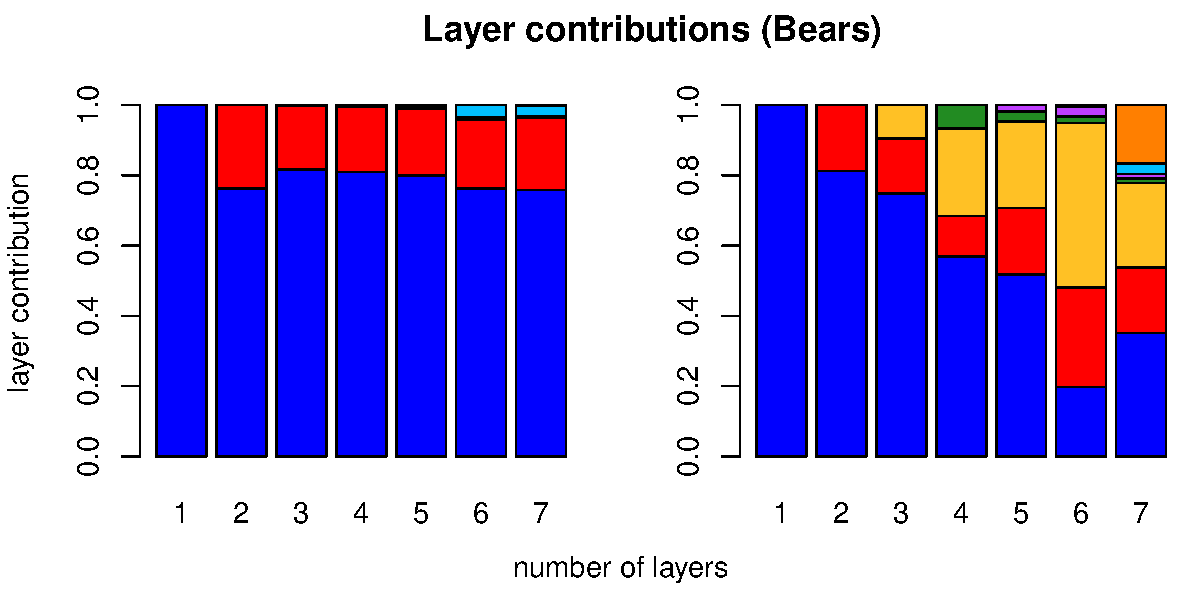
\includegraphics[width=\textwidth]{figs/bears/bears_laycon_barplots.pdf}}
	\fi
	\caption{
	Layer/cluster contributions (i.e., how much total covariance is contributed by each layer/cluster), 
	for all layers estimated in runs using $K = 1$ through 7 
	for the spatial model (left),
	and for all clusters using the nonspatial model (right).
	For each value of $K$ along the x-axis, there are an equal number of contributions plotted.
	Colors are consistent with Fig \ref{bear_K3}.
    }\label{bear_laycon}
\end{figure}

The results partition the sampled bears into two main groups:
one (red) to the east of the Rocky Mountains, 
which also occurs in Alaska,
the other primarily west of the Rockies (blue)  (Fig \ref{bear_K3}a).
The disjointed range of the blue layer likely reflects the fact
that Canada was not sampled, 
and so the red layer may extend
through the intervening (unsampled) northern Great Plains and Canadian Shield, 
with the blue layer presumably then stretching up into British Columbia.

The spatial models have strong statistical support 
up until around $K=5$ or 6 (Fig \ref{bear_xvals}),
but additional spatial layers beyond $K=2$ contribute little to total covariance (Fig \ref{bear_laycon}).
% However, upon examining layer contributions (Fig \ref{bear_laycon}),
% it is clear that the additional spatial layers beyond $K=2$ are contributing only a very small amount toward total covariance between individuals.
The locations of admixed individuals 
% between the two layers provide information about a possible zone of contact and migration between these groups 
% along the northwestern coast of North America and near the Cascade Range in the northern U.S.
are consistent with a scenario of postglacial expansion from two refugia, 
one in the American Southwest and one in the American Southeast, 
meeting near the Northwest coast of North America and the Cascade Range.
However, lack of any samples from Canada and Mexico, 
and lack of denser sampling across northern North America, 
make more detailed interpretations untrustworthy.
%In addition, our model is not an explicit test of any demographic scenario, 
%and also uses a dataset that consists solely of nuclear (rather than
%mitochondrial) DNA. WHY DO WE CARE about BEAR MTDNS

Results from the nonspatial model and from the ADMIXTURE analyses 
clearly exhibit the tendency of nonspatial clustering algorithms 
to describe continuous spatial patterns of divergence 
using gradients of admixture between clusters.
For example, in Fig \ref{bear_K3}b, 
the third cluster (in gold) exhibits a clear East-West gradient that 
overlays the discrete structure between the Southwest cluster and the Southeast.
The results from ADMIXTURE are are not identical to 
those obtained using the nonspatial model, 
but they do show the same tendency: 
e.g., at $K=3$ 
-- the preferred model from the cross-validation 
analysis shown in Fig \ref{bear_admix_CVerrors} -- 
ADMIXTURE splits the westernmost Alaskan samples 
out of the cluster with the eastern samples, 
and at $K=4$, it subdivides the eastern cluster 
into two geographically partitioned groups (Fig \ref{bear_admixture}).
Interestingly, for the nonspatial model implemented in ADMIXTURE, 
the preferred model has a smaller $K$ ($K=3$) than that of the 
spatial model with best cross-validation performance in \texttt{conStruct} ($K=5$ or 6). 
However, comparing results of the two methods, it is clear that even at $K=3$, 
ADMIXTURE is invoking clusters to describe what seems to be, 
and is well described by \texttt{conStruct} as, 
a continuous spatial pattern of genetic variation. 
The third cluster (shown in gold in Fig \ref{bear_admixture}b), 
shows  strong spatial autocorrelation in admixture proportions, 
as would be expected if it is describing continuous spatial differentiation.

Across all values of $K$ for which we ran \texttt{conStruct},
we see strong support for the spatial model over the nonspatial model (Fig \ref{bear_xvals}).
% indicating the isolation by distance seems to be a prominent feature of the data.
This pattern may resolve a discrepancy between our results and 
previous analyses that split Alaskan and British Columbian bears out 
into their own cluster with an inferred Beringian glacial refugium
\cite{Byun1997,Stone2000,Puckett2015}.
Our model, which explicitly incorporates a spatial decay of relatedness, 
allows somewhat genetically differentiated individuals 
that are sampled far from one another to belong to the same layer,
instead of splitting these individuals out into successive clusters 
(e.g., Fig \ref{bear_sp_pies}d vs \ref{bear_nsp_pies}d).

%%%%%%%%%
\section*{Discussion}

% The difficulty of dispersing across geography makes
% the pattern of isolation by distance ubiquitous in nature.
% % this is unsurprising, as mating opportunities are distance-limited in most species.
% % This common pattern can flummox 
% Commonly used clustering methods
% must employ a possibly large number of discrete clusters
% to describe this simple pattern.
% The resulting spurious clusters can have implications for 
% downstream analysis and interpretation of genetic data, 
% including conservation management decisions. 

In this paper, we have presented a statistical framework, \texttt{conStruct}, for simultaneously 
modeling continuous and discrete patterns of population structure.
By employing the sensible default assumption
that relatedness ought to decay with geographic distance, even within a population, 
we avoid erroneously ascribing population differentiation to discrete population clusters.
To aid comparison between models,
we present a cross-validation approach 
as well as a way to describe the contribution of each spatial layer to the model
(but caution against overly strict interpretation of either).

The method performs well on simulated data:
we accurately infer the admixture proportions used to simulate the data 
and accurately pick the simulating model as the best model using our cross-validation procedure.
Two empirical applications of \texttt{conStruct} to samples of North American poplars and black bears
yield reasonable results,
and demonstrate that,
by acknowledging isolation by distance,
real datasets can be better described using fewer layers.

The proposed method combines the utility of model-based clustering algorithms 
with a biologically realistic model of isolation by distance.
We anticipate that \texttt{conStruct} will be useful for identifying populations 
and determining samples' ancestry in and across them, 
especially when the populations exhibit spatial patterns of relatedness.

\paragraph{Comparison to nonspatial model-based clustering}
Above, we showed that 
(a) the nonspatial \texttt{conStruct} model recapitulates results of 
other, commonly-used nonspatial clustering methods,
and 
(b) \texttt{conStruct} can concisely capture spatial structure, which
will be common within populations.
Given this, when should methods without spatial capability be used?
One advantage these have over \texttt{conStruct} is speed when the number of samples is large.
Although \texttt{conStruct}'s computation time is independent
of the number of loci included in the dataset 
(after the initial calculation of the allelic covariance), 
it currently scales poorly with number of samples.
The computationally limiting step is the inversion of the parametric covariance, 
% actually it is like O(n^2.3) but I don't know which algorithm STAN uses
% which is an operation of order $O(n^3)$, 
which scales more than quadratically with the number of samples,
whereas computation time for, e.g., STRUCTURE, 
scales linearly with number of samples.
Our speed, on datasets with large sample sizes, 
could be improved by adopting rank-one updates 
to the inverse of the covariance matrix 
(e.g., \cite{woodbury1950,sherman_morrison1950})
when updating a sample's admixture proportions, 
which alters only a single row/column of the covariance matrix. 
We have not implemented this yet, 
as it would likely mean losing the ability to do efficient,  
Hamiltonian Monte Carlo sampling of our parameters.

For a relatively small number of samples, 
\texttt{conStruct} can be much faster than existing nonspatial Bayesian clustering methods.
On a desktop machine, using a single 4.2 GHz Intel Core i7 processor, 
an analysis of the black bear dataset (78 samples, 21,000 loci) 
running \texttt{conStruct}'s spatial model with 4 layers for 5,000 MCMC iterations 
(which was more than sufficient for convergence) 
took 2.8 hours.
On the same machine and dataset, 
a fastSTRUCTURE \cite{fastStructure} run with $K=4$ took 90.2 hours.
However, for a large number of samples, 
fastSTRUCTURE might be faster.
And, for almost any dataset of any size, 
the maximum likelihood algorithm implemented in ADMIXTURE 
is also quite a bit faster than \texttt{conStruct}; 
Running ADMIXTURE on the bear dataset over all values of $K$ from 1 to 7, 
including 50-fold cross-validation for each value of $K$, took only 6.6 minutes.


\paragraph{Choosing the ``best" number of layers}
Although we recognize the utility of choosing a single, ``best'' value of $K$, 
and using only that analysis to communicate results, 
we emphasize that 
% there is no true best value of $K$. 
% HOW ABOUT: there is no truth.
the choice of best $K$ is always relative to the data in hand
and the questions to be answered.
%This means both that sampling different individuals or loci 
%from the same populations may yield a different ``best" $K$, 
From a statistical perspective, unless the data were generated under the model itself,
the support for larger values of $K$ is likely to increase with increasing amounts of data.
%(although perhaps only logarithmically).
In the limit of infinite data, the best value of $K$ 
may be the number of samples included in the dataset \cite{Patterson2006}.

From a biological perspective, 
it is important to stress that patterns of relatedness between individuals and populations 
are shaped by complex spatial and hierarchical processes.
All individuals within a species (and indeed, all individuals across all species), 
are related to one another in some way, 
and summarizing that relatedness with a single value of $K$ may be reductive or misleading.
We therefore encourage users to perform analyses across different values of $K$ and 
observe which layers split out at what levels 
(this is conceptually similar to taking successively shallower
cross-sections of the population phylogeny), 
and also to take the results of the proposed cross-validation procedure with a large grain of salt.
Calculating layer contributions may also be a useful heuristic, 
as it can reveal layers with statistical support but small biological import.

Although we believe our model adds spatial realism to the groups used by clustering methods,
it is important to note that the layers detected by our method 
do not necessarily correspond  to distinct, ancestral populations; 
nor does a non-zero admixture proportion indicate that admixture 
(i.e. gene flow) must have occurred. 
Both groupings and admixture proportions
should be viewed as hypotheses that should be subject to further testing
(see \cite{Falush:16} for an in-depth discussion of these points).

\paragraph{Implications for management and conservation}
Because isolation by distance is common, 
a likely result of applying \texttt{conStruct} to existing data is that some
populations previously identified using nonspatial clustering methods 
may be collapsed into each other.  
This ``lumping'' might better reflect biological reality, 
but may also have implications for management decisions and conservation policy, 
both of which are often predicated on the identification of discrete ``management units'' (MUs) 
identified using genetic data \cite{Moritz1994,Waples_1998,Moritz_etal_2002}.

It is therefore important to stress that individuals sampled from the same \texttt{conStruct} layer 
may be quite genetically diverged from one another, 
perhaps especially at loci underlying adaptive traits, % \citep{toews2016plumage}, 
and that a \texttt{conStruct} layer may still contain multiple distinct MUs worthy of independent protections.  
Alternatively, the inclusion of multiple MUs into a single \texttt{conStruct} layer 
may occur if these populations are currently 
(or were recently) exchanging migrants, 
and thus might emphasize the importance of maintaining habitat corridors between demes, 
or of implementing an integrated conservation plan across multiple demes within a layer.
% Conversely, two populations that are easily distinguishable based on abundant genetic data
% need not be strongly differentiated --
% population assignment is not a replacement for absolute measures of genetic divergence.

\paragraph{Allelic or genetic covariance?}
The choice of allelic covariance, rather than genetic covariance,
was motivated by two considerations.
First, it captures within-population variance in a manner more suited to the modeling approach here,
which led to better performance on test data.
Second, it is less affected by sample configuration --
the genetic covariance is calculated after subtracting the mean from the entire sample,
which is more strongly affected by densely sampled locations.
However, note that allelic covariance is more affected by singleton sites
than the standard genetic covariance,
so it may be advisable to filter these prior to analysis
if they are likely to contain a large percentage of errors \cite{linck_battey2017}.

\paragraph{Caveats and considerations}
There are a few important caveats to consider in the interpretation of \texttt{conStruct} results. 
First, we have modeled allelic covariance within a layer as a spatial process.
Although there is flexibility built into the model about the shape of that covariance, 
inference may be misleading if the sampling geography departs radically from the way 
the sampled organisms disperse (or have dispersed) on their landscape.
For example, if we were to run a \texttt{conStruct} analysis using geographic distances between 
sampled individuals of greenish warblers \cite{Irwin2001} or \textit{Ensatina} salamanders \cite{wake_schneider1998} 
--- two canonical examples of rings species --- 
we might get misleading results.
This is because distance between locations on either side of the species' distributions
(across the Tibetan plateau and the Central Valley, respectively) 
is not representative of the path traversed in the coalescent of a pair of alleles sampled at those locations.

A second caveat is that, in some instances, 
membership in the same layer may not mean that samples are particularly related.
If covariance within a layer decays sharply with distance, 
and the layer-specific relatedness parameter $\phi^{(k)}$ is low, 
individuals separated by a large spatial distance may be in the same layer but have very low pairwise relatedness.
It is possible that this is happening in Fig \ref{populus_sp_pies}. 
At $K=3$, the southernmost populations of \textit{P. trichocarpa} are in the gold layer, 
whose other neighbors are to the north, with an intervening group of populations in the red layer, 
and at $K=5$, those southernmost samples split out and become their own layer.
Again, we encourage users to run analyses across multiple values of $K$, 
and to examine the spatial covariance functions within layers when interpreting results.

\paragraph{Extensions and future directions}
There are several ways in which the model described in this paper might be extended or improved.  
For example, we currently assume that all layers within a model are equally unrelated 
(a star population phylogeny, although the branches can have different lengths thanks to the $\phi^{(k)}$ parameter), 
similar to the F-model of \cite{falush2003}.
However, we could extend the existing model by implementing 
a relatedness structure between the layers by, for example, 
estimating a population phylogeny between them
(e.g, \cite{treemix}).

In addition, here we have assumed that samples have known geographic coordinates, 
and that they draw ancestry from layers only at those sampled locations. 
A natural extension would be to attempt to ``geo-locate'' 
the ancestry of samples without geographic coordinates \cite{Wasser2004}. 
We could also imagine letting samples draw ancestry from other geographic coordinates, 
as we have done in a previous approach \cite{spacemix} to model long distance dispersal. 
We could even allow entire layers to bud off of a particular location on another layer. 
This would enable more explicit modeling of range expansion or domestication, 
in which a set of individuals are thought to have ancestry that originated from
a particular geographic location embedded in a larger pattern of isolation by distance.

A final direction would be to model relatedness within a layer as a spatiotemporal process, 
in which covariance decays both with distance in space and in time.  
As the number of genotyped historical or ancient samples increases, 
it is becoming possible to ask whether there is genetic continuity at a point in space across time, 
or whether populations are being replaced \cite{lazaridis_ancient_2014, Haak2015, slatkin_racimo2016, Nielsen2017, Schraiber2017}.
However, we expect allele frequencies to change through time in a population, 
even without replacement, simply due to drift.
Therefore, a natural way to test for population replacement is to estimate the rates 
at which relatedness within a layer decays with time in the same way we do in the current model with space, 
in which case a change in discrete population structure across space is comparable to population replacement across time.

\section*{Materials and Methods}

% \section*{Appendix}
% \pagenumbering{gobble}
% \renewcommand{\theequation}{A\arabic{equation}}
% \setcounter{equation}{0}
% \renewcommand{\thetable}{A\arabic{table}}
% \setcounter{table}{0}
% \renewcommand{\thefigure}{A\arabic{figure}}
% \setcounter{figure}{0}
% \renewcommand{\thesection}{A\arabic{section}}
% \setcounter{section}{0}


\section*{Model rationale} \label{rationale}

\subsection*{Drift, admixture, and space}
Here we sketch a simple model of allele frequencies and their
covariances, to justify the form given in the main text.

\paragraph{Drift} 
We first provide a simple model of allele frequencies within a layer. 
Imagine a sample $i$ that draws all of its ancestry from layer $k$.
The allele frequency in sample $i$ at locus $\ell$, denoted $F_{i,\ell}$, can be
written as the sum
\begin{equation}
F_{i,\ell} = \epsilon_{\ell} + \Delta^{(k)}_{\ell} +
\Delta^{(k,i)}_{\ell} + \Delta^{(i)}_{\ell} .
\label{drift_terms_no_admix}
\end{equation}
The first term is the ancestral allele frequency $\epsilon_\ell$ shared by all samples; 
the second is the deviation from that ancestral frequency 
due to drift in the ancestral population of the $k$th layer,
which is shared by all samples within the layer. 
The third term is the deviation of the $i$th sample away from the $k$th layer mean 
due to the spatial process of drift and migration within the layer.
The final term is the deviation specific to the $i$th sample,
which captures drift not shared by all samples at the population level
(i.e., subpopulation-specific drift due to, e.g., inbreeding). 
We will assume that these four deviations are all uncorrelated with each other.

If we have two samples $i$ and $j$ drawn from layer $k$, 
their covariance across loci will be 
\begin{equation}
\text{Var}(\epsilon) +  \text{Var}\left( \Delta^{(k)} \right) +
\text{Cov}(\Delta^{(k,i)}_{\ell},\Delta^{(k,j)}_{\ell}) + \delta_{i=j} \text{Var}\left( \Delta^{(i)} \right),
\end{equation}
where the quantity $\delta_{i=j}$ is an indicator variable that equals 1 when $i$ is equal to $j$ and 0 otherwise, 
as in Eq.\ \eqref{cross_layer_covariance}.

\paragraph{Admixture} 
The model above describes the simple case 
in which samples draw 100\% of their ancestry from only a single layer each. 
To accommodate admixture between layers, 
we model sampled genomes as drawn from
allele frequencies that are weighted averages of the local frequencies in each layer
from which they draw ancestry.
The weights, $w^{(k)}_{i}$, describe the
``admixture proportion'' of sample $i$ in layer $k$.
(Note that $\sum_{k=1}^K w^{(k)}_{i} = 1$ for each $i$.)
These can be interpreted as the proportion of the genome in the $i$th
sample that came from the $k$th layer 
(or the probability that an allele at a locus is drawn from layer $k$).
The allele frequency in the $i$th sample at the $\ell$th locus can therefore be written as:
\begin{equation}
F_{i,\ell} = \epsilon_{\ell} + \sum\limits_{K} w^{(k)}_{i}\left( 
  \Delta^{(k)}_{\ell} + \Delta^{(k,i)}_{\ell}\right) + \Delta^{(i)}_{\ell}	 ,
\label{drift_terms_admix}
\end{equation}
and so the covariance between $i$ and $j$ across loci is
\begin{equation}
\Omega_{i,j} = \text{Var}(\epsilon) + \sum_{k=1}^K w^{(k)}_iw^{(k)}_j
\left(
  \text{Var}\left( \Delta^{(k)} \right) +
\text{Cov}(\Delta^{(k,i)}_{\ell},\Delta^{(k,j)}_{\ell}) 	\right) +
\delta_{i=j} \text{Var}(\Delta_i) .
\label{admixed_spatial_cov}
\end{equation}

\paragraph{Space}
Under our nonspatial model, 
we assume that $\text{Cov}(\Delta^{(k,i)}_{\ell},\Delta^{(k,j)}_{\ell})=0$,
so that the only additional covariance between $i$ and $j$ 
(above that induced by a shared ancestral frequency at each locus)
is due to the drift in the ancestral population of their layer 
(the variance of which is $\phi^{(k)}$). 
Under our spatial model we assume that some of the covariance in allele frequencies
between $i$ and $j$ decays as a function of the geographic distance
between the pair, $D_{i,j}$,
so that 
\begin{equation}
\text{Cov}(\Delta^{(k,i)}_{\ell},\Delta^{(k,j)}_{\ell}) = \alpha^{(k)}_0 \times \left(\text{exp} \left(  -(\alpha^{(k)}_D D_{i,j})^{\alpha^{(k)}_2}\right) \right) .
\end{equation}
We note that this form is chosen for its flexibility, 
and not because it matches any explicit population genetic model of isolation by distance. 


\section*{Allelic covariance}\label{allelic_cov}
To see why equations
\eqref{eqn:first_allelic_cov} and \eqref{allelic_covariance}
for the allelic covariance are equivalent,
pick a random locus and
let $A$ and $B$ be randomly drawn alleles at that locus from populations $i$ and $j$ respectively.
%If $i=j$, then these are chosen \emph{without} replacement.
Suppose these are each coded as `0' or `1' (where `0' denotes a reference allele),
but we randomly ``flip'' this coding, so that we let $X=A$ and $Y=B$ with probability 1/2,
but otherwise we let $X=1-A$ and $Y=1-B$.
These are $X_i$ and $X_j$ in equation \eqref{eqn:first_allelic_cov},
so that $\widehat{\Omega}_{i,j} = \cov[X,Y]$. 
%Sampling without replacement makes the statistic insensitive to sample size,
The random allele flipping makes the value of $\widehat{\Omega}$ 
independent of the choice of reference allele.
By conditioning on the flip,
and using the fact that $\E[X] = \E[Y] = 1/2$,
Eq.\ \eqref{allelic_covariance} comes from the observation that
\begin{align} \label{eqn:cov_xy}
\cov[X,Y] % &= \E[XY] - 1/4 = (1/2)\E[AB + (1-A)(1-B)] - 1/4\\\notag
    &= \E[(A-1/2)(B-1/2)] .
\end{align}

Thanks to averaging over choice of alleles,
the within-population allelic variance in sample $i$, $\widehat Omega_{i,i}$,
is the variance of a series of Bernoulli($1/2$) draws across loci,
and therefore $\widehat{\Omega}_{i,i} = 1/4$ for every sample $i$.
Averaging over choice of reference allele therefore removes some information 
about factors acting within populations that might otherwise leave signatures in, 
e.g., the genetic covariance, 
such as population size, extent of inbreeding, and history of bottlenecks.  
However, as our model is focused on modeling 
\emph{co}variances between samples as the outcome of some spatial process, 
we count this a minor loss.


%The factor of $\delta_{i,j}/(N_i-1)$ comes from the fact that if $i=j$,
%then $\E[AB]$ is the probability that both alleles drawn without replacement are reference,
%which is $f_i^2 n/(n-1)$.

%and reflects the covariance between individual alleles drawn from within the population.
%To compute it from allele frequencies, first
%write $N_i$ for the number of chromosomes sequenced in the $i^\text{th}$ sample.
%The \emph{sample frequency} at locus $\ell$ in sample $n$, denoted $f_{n,\ell}$, 
%is calculated by first arbitrarily choosing one of the observed alleles at locus $\ell$ to count, 
%then dividing the number of observations of that counted allele by the total number of chromosomes genotyped at that locus
%in sample $n$.


\paragraph{Likelihood}
If allele frequency deviations are well approximated by a Gaussian, 
their sample allelic covariance is a sufficient statistic,
so that calculating the likelihood of their sample allelic covariance is the same as 
calculating the probability of the frequency data up to a constant. 
We can therefore model the covariance of the sample allele frequencies, $\widehat{\Omega}$, 
as a draw from a Wishart distribution with degrees of freedom equal to 
the number of loci $L$ across which the sample allelic covariance is calculated:
\begin{equation}
\widehat{\Omega} \sim \mathcal{W}\left( L\Omega, L	\right) 
\label{wishart}
\end{equation}
where $\mathcal{W}$ is the Wishart likelihood function.

A benefit of directly modeling the sample allelic covariance is that, 
after the initial calculation of the sample covariance matrix,
the computation time of the likelihood is not a function of the number of loci,
so inference can theoretically be done using whole genome data.


\section*{Models, parameters, and priors}\label{model_app}

\paragraph{Spatial versus nonspatial}
In this paper, we discuss two types of models, spatial and nonspatial, 
each of which can be implemented with different numbers of layers/clusters.
The spatial model is parameterized as in Eq.\ \eqref{admixed_spatial_cov},
and the nonspatial model
is a special case of the spatial model with all $\alpha$ parameters is set to 0.
% is described in Eq.\ \eqref{admixed_discrete_covariance}.  % that's not the right eq'n
The nonspatial model therefore has $3K$ fewer parameters than the spatial model,
because there are three $\alpha$ parameters that describe the continuous differentiation effect of distance in each layer.

\paragraph{Single layer}
Each of these models can be run with a single layer ($K=1$), 
in which case the layer-specific covariance parameter $\phi^{(k)}$ 
and the global covariance parameter $\gamma$ become redundant.
The single-layer model is therefore a special case of the multi-layer model, 
in which we set $\phi$ to zero.
For the spatial model, the single-layer parametric covariance is:
\begin{equation}
\Omega_{i,j} = \text{Var}(\epsilon) + 
\alpha^{(k)}_0 \times \left(\text{exp} \left(  -(\alpha^{(k)}_D D_{i,j})^{\alpha^{(k)}_2}\right) \right)	 +
\delta_{i=j} \text{Var}(\Delta_i), 
\label{admixed_continuous_cov}
\end{equation}
and for the nonspatial model, it is:
\begin{equation}
\Omega_{i,j} = \text{Var}(\epsilon) + \delta_{i=j} \text{Var}(\Delta^{(i)}) .
\label{admixed_discrete_covariance}
\end{equation}

\paragraph{Priors}
We use a Bayesian approach to parameter inference.
A table of all parameters, their descriptions, and their priors is given in Table \ref{tab:param_prior_tab}.

\begin{table}
\begin{centering}
\ifincludefigs
\begin{tabular}{| >{\centering\arraybackslash}m{2.1cm} | m{5.2cm} | >{\centering\arraybackslash}m{5.1cm} |}
	\hline
	\textbf{Parameter} & \centering{\textbf{Description}} & \textbf{Prior}\\ \hline
	$\boldsymbol{\gamma}$ & 
		global covariance due to shared ancestral frequency & 
		$\gamma \sim \mathcal{N}(\mu = \text{Var}(\bar{f}), \sigma = 0.5)$\\ \hline
	$\boldsymbol{\alpha^{(k)}_0}$ & 
		controls the sill of the covariance matrix in layer $k$& 
		$\alpha^{(k)}_0 \sim \mathcal{N}(\mu = 0, \sigma = 1)$\\ \hline
	$\boldsymbol{\alpha^{(k)}_D}$ & 
		controls the rate of the decay of covariance with distance in layer $k$& 
		$\alpha^{(k)}_D \sim \mathcal{N}(\mu = 0, \sigma = 1)$\\ \hline
	$\boldsymbol{\alpha^{(k)}_2}$ & 
		controls the shape of the decay of covariance with distance in layer $k$ & 
		$\alpha^{(k)}_2 \sim U(0,2)$\\ \hline
	$\boldsymbol{\eta_i}$ & 
		the nugget in population $i$ (population specific drift parameter)  & 
		$\eta_i \sim \mathcal{N}(\mu = 0, \sigma = 1)$\\ \hline
	$\boldsymbol{\phi^{(k)}}$ & 
		layer-specific shared drift in layer $k$ &
		 $\phi^{(k)} \sim \mathcal{N}(\mu = 0, \sigma = 1)$\\ \hline
	$\boldsymbol{w_i}$ &
		admixture proportions sample $i$ draws across $K$ layers &
		$w_i \sim \text{Dir}(\alpha_{1} ... \alpha_{K}=0.1)$  \\ \hline
	\hline
\end{tabular}
\fi
\caption{
List of parameters used in the \texttt{conStruct} model, along with their descriptions and priors.
The mean of the Normal prior on $\gamma$, $\text{Var}(\bar{f})$, is the variance of the sample mean allele frequencies across loci.
}\label{tab:param_prior_tab}
\end{centering}
\end{table}

\section*{Cross validation}\label{Xvalidation}

We employ Monte Carlo cross-validation approach for model comparison \cite{picard1984}. 
This procedure generates a mean predictive accuracy for each model and each value of $K$, 
as well as a confidence interval around that mean,
which can then be used for model comparison or selection.
Briefly, we follow the following procedure:
\begin{enumerate}
\item For each of $X$ replicates:
	\begin{enumerate}
		\item partition the allele frequency data into a 90\% ``training'' partition ($F^x_1$) and a 10 \%``testing" partition ($F^x_2$) \label{partition}
		\item run our inference procedure on the training partition to estimate model parameters $\theta_{mk}$ for: \label{inference}
			\begin{enumerate}
				\item $m$: the spatial and the nonspatial model
				\item $k$: the number of layers/clusters 1 through $K$
			\end{enumerate}	
	\item calculate the mean log likelihood of the testing data partition  
	over the posterior distribution of training-estimated parameters for each model 
	($\bar{\mathcal{L}}(F^x_2 \mid \theta_{mk})$, henceforth $\bar{\mathcal{L}}_{xmk}$) \label{lnL}
	\item generate standardized mean log likelihoods, $\mathcal{Z}_{xmk}$, across models: \label{standardize}
		\begin{enumerate}
			\item identify the highest mean log likelihood, $\bar{\mathcal{L}}^\text{max}_{xmk}$
			\item subtract $\bar{\mathcal{L}}^\text{max}_{xmk}$ from $\bar{\mathcal{L}}_{xmk}$ across all models,
				such that the standardized log likelihood, $\mathcal{Z}_{xmk}$, of the best model is 0,
				and less than 0 for all inferior models. 
		\end{enumerate}
	\end{enumerate}
\item For each model (i.e., each combination of $m$ and $k$) calculate 
	the mean ($	\bar{\mathcal{Z}}_{mk} $) standardized log likelihood of the testing data partition across $X$ replicates, 
	as well its standard error ($SE_{\bar{\mathcal{Z}}_{mk}}$) and
        95\% confidence interval ($\bar{\mathcal{Z}}_{mk} \pm 1.96 \times SE_{\bar{\mathcal{Z}}_{mk}}$).
\end{enumerate}

\gb{If the spatial coordinates of the loci in the genome are known, 
the training/testing partitioning should be designed to accommodate linkage disequilibrium (LD).
Loci in strong LD do not represent independent instantiations of the coalescent process, 
so if loci from a single linkage block are randomly split into both training and testing partitions, 
the independence of the test in the testing partition will be compromised 
(e.g., the parameters estimated from the training partition 
might be describing process heterogeneity or noise 
in a region of the genome that also has loci included in the testing partition).
If genomic position or LD between SNPs is known, 
the best practice for cross-validation is to make sure that 
no loci in the testing dataset are in strong LD with, 
or spatially proximate to, loci in the testing dataset.}


\section*{Calculating layer contributions}\label{layer_contribution}

Let $A$ and $B$ be randomly chosen alleles from samples $i$ and $j$ respectively,
at a randomly chosen locus 
(if the two populations are the same, then choose without replacement).
Then, if we let $U=2(A-1/2)$ and $V=2(B-1/2)$,
since $U$ and $V$ take the values $\pm 1$,
so as in Eq.\ \eqref{eqn:cov_xy},
$$\begin{aligned}
\E[UV]
        &= \P\{ U=V \} - \P\{ U \neq V \} \\
        &= 2 \P\{ U=V \} - 1 \\
        % &= 1 - 2 \P\{ U \neq V \} .
        &= 2 \P\{ A=B \} - 1 
\end{aligned}$$
To translate, $\P\{ U=V \}$ is the probability that the alleles from our two focal samples agree with each other,
while $\P\{ U \neq V \}$ is the probability that they disagree.
This implies that $\E[UV] = 1 - 2 \pi_{ij}$, 
where $\pi_{ij}$ is the probability that two randomly chosen alleles differ, 
which is the genetic divergence.

Now, here is a generative model that gives us the form of the covariance we have postulated.
To decide whether or not $A$ and $B$ will agree,
first each sample randomly chooses a layer: call these layers $I$ and $J$.
The probability that $A$ chooses layer $k$ is $\P({I=k})=w_i^{(k)}$, 
the $i$th sample's admixture proportion in the $k$th layer.
The same holds true for $B$.
If they do not choose the same layer, the probability that they agree is $p_\gamma$.
If they do choose the same layer, 
then they agree with a probability $p_\gamma + q^{(k)}_{ij}$ that depends on their distance apart.
By the above,
the probability of agreement is $\P\{A=B\} = 2 \cov[A,B] + 1/2$,
and so
$$\begin{aligned}
    p_\gamma &= (2 (\gamma + \delta_{ij} \eta_i) + 1/2) \\
    q^{(k)}_{ij} &= \left(2 \alpha_0^{(k)} \exp\left( - \left(\alpha_D^{(k)} D_{ij}\right)^{\alpha_2^{(k)}} \right) + 2 \phi^{(k)}  + 1/2 \right) .
\end{aligned}$$

One way to summarize the contribution of each layer is to partition the probability of agreement
into contributions due to agreement ``in" each layer.
So, the contribution from layer $k$ to agreement between $i$ and $j$ is 
$w_i^{(k)} w_j^{(k)} q^{(k)}_{ij} / (p_\gamma + \sum_{k=1}^K w_i^{(k)} w_j^{(k)} q^{(k)}_{ij})$,
which is the probability, given that they agree, that they agree thanks to layer $k$.
Similarly, the ``background" contribution is $p_\gamma / (p_\gamma + \sum_{k=1}^K w_i^{(k)} w_j^{(k)} q^{(k)}_{ij})$.
Because our signal comes from \emph{variation} in covariance, we omit
the $p_\gamma$ terms. 
Stated in this way, this quantity is the
relative contribution of the $k$th layer to the (model-based) kinship
coefficient between $i$ and $j$.

This suggests defining the overall contribution of layer $k$ to agreement, $\xi^{(k)}$, 
to be the average of that quantity over $i$ and $j$:
\begin{equation}
\xi^{(k)} = 
	\sum\limits_{i=1}^{N}
		\sum\limits_{j=i}^N
			w^{(k)}_iw^{(k)}_j 
				\left(	
					2\alpha^{(k)}_0 
						\left( \text{exp} 
							\left( -(\alpha^{(k)}_D D_{i,j}) ^ {\alpha^{(k)}_2}\right) 
						\right) + 2\phi^{(k)} + \frac{1}{2}
				\right) ,
\label{abs_layer_contribution}
\end{equation}
which is that layer's contribution to agreement between samples 
summed over the upper triangle (excluding the diagonal) of the covariance matrix.
We define the contribution of the $k$th layer, $\Xi^{(k)}$, 
as the relative contribution of the $k$th layer to total agreement:
\begin{equation}
\Xi^{(k)} = 
\frac{\xi^{(k)}}
	{\sum\limits_{k=1}^{K}
	    	\xi^{(k)}} .
\label{rel_layer_contribution}
\end{equation}
This is the quantity that is plotted in, e.g., Figures \ref{simK1_laycon} and \ref{bear_laycon}.


\section*{Simulation details}\label{sim_details}
We wished to simulate data under a model that had some biological realism, 
but at the same time had unambiguous true admixture proportions 
(so as to test the behavior of the method).
This second requirement precluded scenarios of, e.g, 
recent secondary contact between populations expanding out of different refugia, 
which would have more biological realism, 
but no unambiguous ancestry proportions for admixed populations.
Here, we describe in more detail the procedure we use to simulate our test dataset, 
using a cartoon schematic with $K=2$ as an example (Fig \ref{sim_setup}).

\begin{figure}[!ht]
	\centering
	\ifincludefigs
		{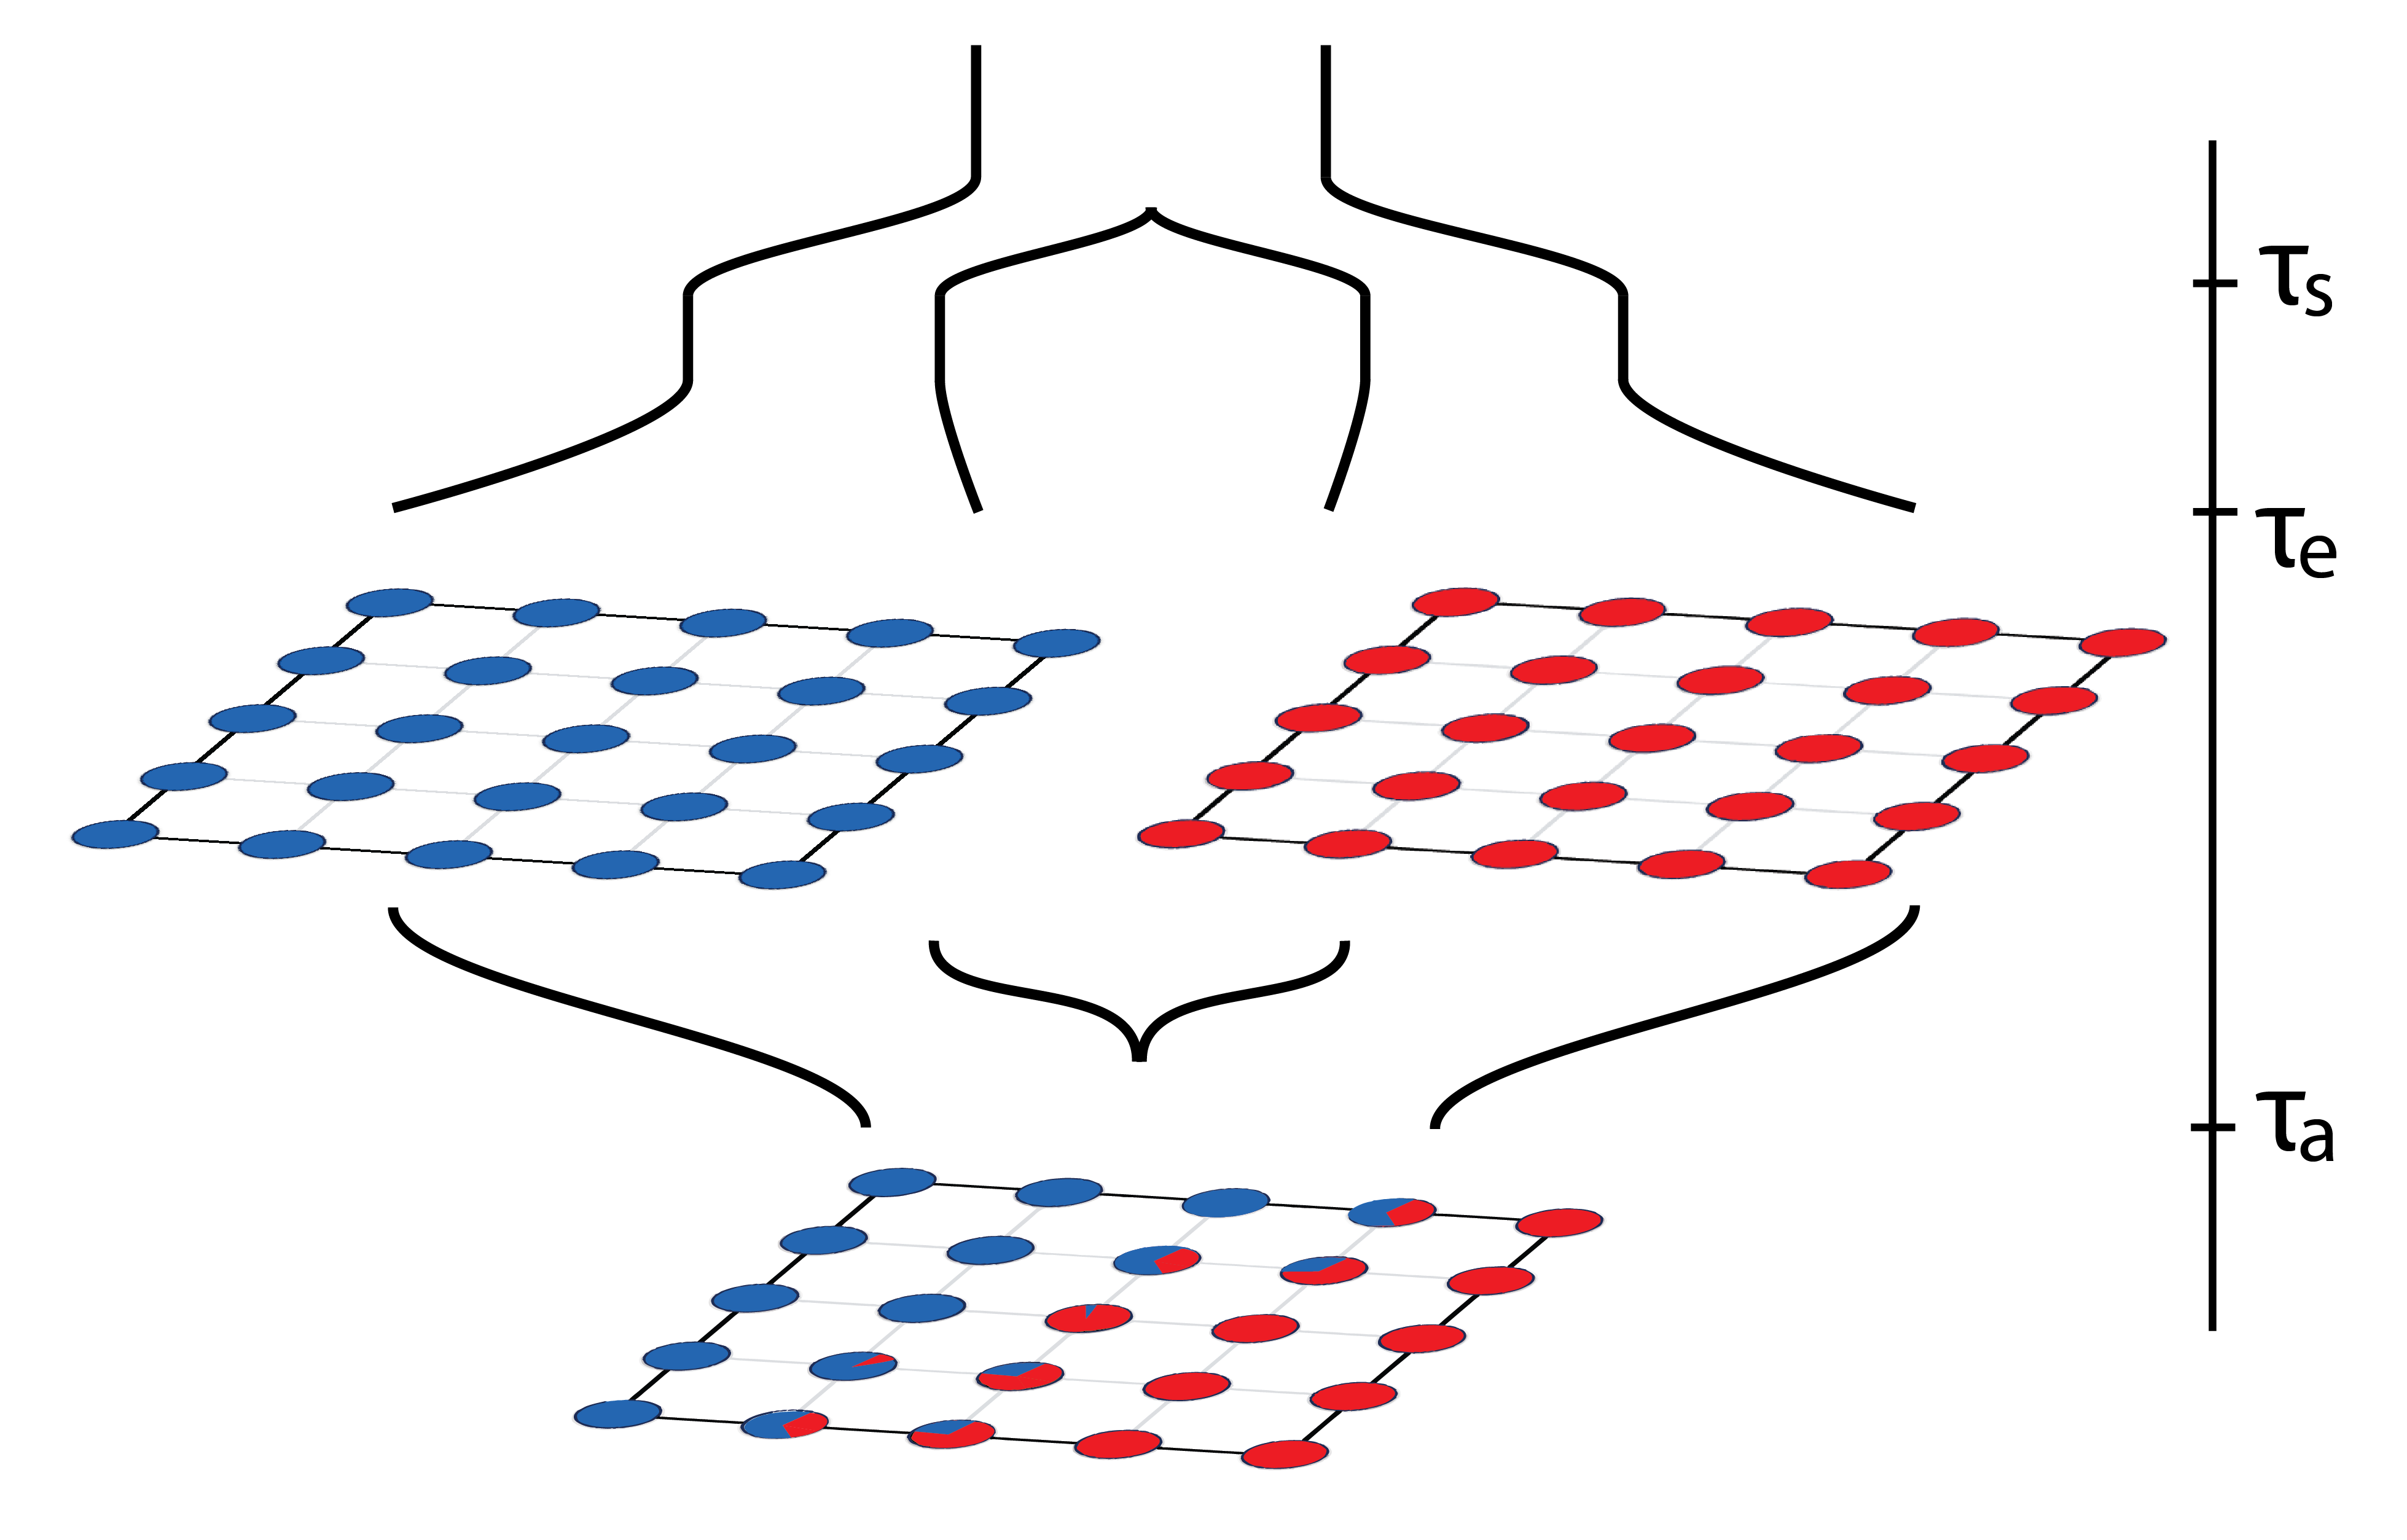
\includegraphics[width=\textwidth]{figs/sims/sim_setup.png}}
	\fi
		\caption{Schematic of how we simulate datasets with continuous and discrete differentiation, using $K=2$ as an example.  
			    Going forward in time, the $K$ populations split from a common ancestor at time $\tau_{\text{s}}$,
			    then expand to each  colonize a lattice of demes with nearest-neighbor symmetric migration at time $\tau_{\text{e}}$,
			    then finally at time $\tau_{\text{a}}$ collapse into a single lattice consisting of demes 
			    with ancestry entirely in one or the other of the populations,
			    or admixed between them.
			    }\label{sim_setup}
\end{figure}

Using the program \texttt{ms} \cite{Hudson2002}, 
we generated discrete population structure by simulating $K$ distinct populations,
each of which split from a common ancestor $\tau_{\text{s}}$ units of coalescent time in the past,
without subsequent migration between them.
Then, to generate continuous differentiation within each population,
at time $\tau_{\text{e}}$ in the past,
each of these discrete populations instantaneously colonizes an
independent lattice of demes,
for which we use a stepping stone model with symmetric migration 
to nearest neighbors (eight neighbors, including diagonals).

Finally, at time $\tau_{\text{a}}$ in the past 
we generate a single dataset 
by collapsing those $K$ discrete lattices into a single grid of demes 
that are admixed to various degrees from these different layers. 
We wish to simulate realistic patterns of admixture 
(and thereby set a more difficult test for the method), 
by generating spatially autocorrelated admixture proportions 
in each diverged population.
To do so, we first place $K$ equidistant points on the circle centered on our lattice.  
These points serve as ``foci" of ancestry in each of the $K$ layers.  
We then calculate the distance from each deme in the sampled lattice to each of these $K$ foci, 
and draw admixture proportions for each deme 
from a Dirichlet distribution for which the concentration parameter 
for deme $i$ in layer $k$ is inversely proportional to the distance between deme $i$ and focus $k$. 
This creates a pattern in which the admixture proportions in a given layer decreases 
with the distance from that layer's focus, 
as might be expected if a spatial process were mediating admixture between diverged populations.

\section*{Acknowledgements}

We thank Marjorie Weber, Yaniv Brandvain, William Wetzel, 
Mariah Meek, Doc Edge, and Matthew Stephens 
for invaluable comments on the method and manuscript, 
as well as Quentin Cronk, who provided input on the \textit{Populus} analyses, 
and Emily Puckett, who provided input on the black bear analyses.
We also thank the attendees at the 2017 SSE Meeting in Portland, OR, 
whose votes determined the name of the method.
\ifsubmissionversion
\else
This work was supported in part by 
the National Science Foundation under award number NSF \#1262645 (DBI) to PR and GC, 
the National Institute of General Medical Sciences of the National
Institutes of Health under award numbers NIH R01-GM108779 to GC,
and the National Science Foundation under award numbers NSF \#1148897 and \#1402725 to GB.
\fi


\newpage
\clearpage
\bibliography{reference.library.tex.bib}


%%% BEGIN IF INCLUDE SUPPLEMENT
\ifincludesupplement

\clearpage
\newpage
\section*{Supplementary Information}
\renewcommand{\theequation}{S\arabic{equation}}
\setcounter{equation}{0}
\renewcommand{\thetable}{S\arabic{table}}
\setcounter{table}{0}
\renewcommand{\thefigure}{S\arabic{figure}}
\setcounter{figure}{0}

% \linespread{1}
% \iffloatsatend
% \processdelayedfloats
% \fi

\clearpage

\begin{figure}
	\centering
		{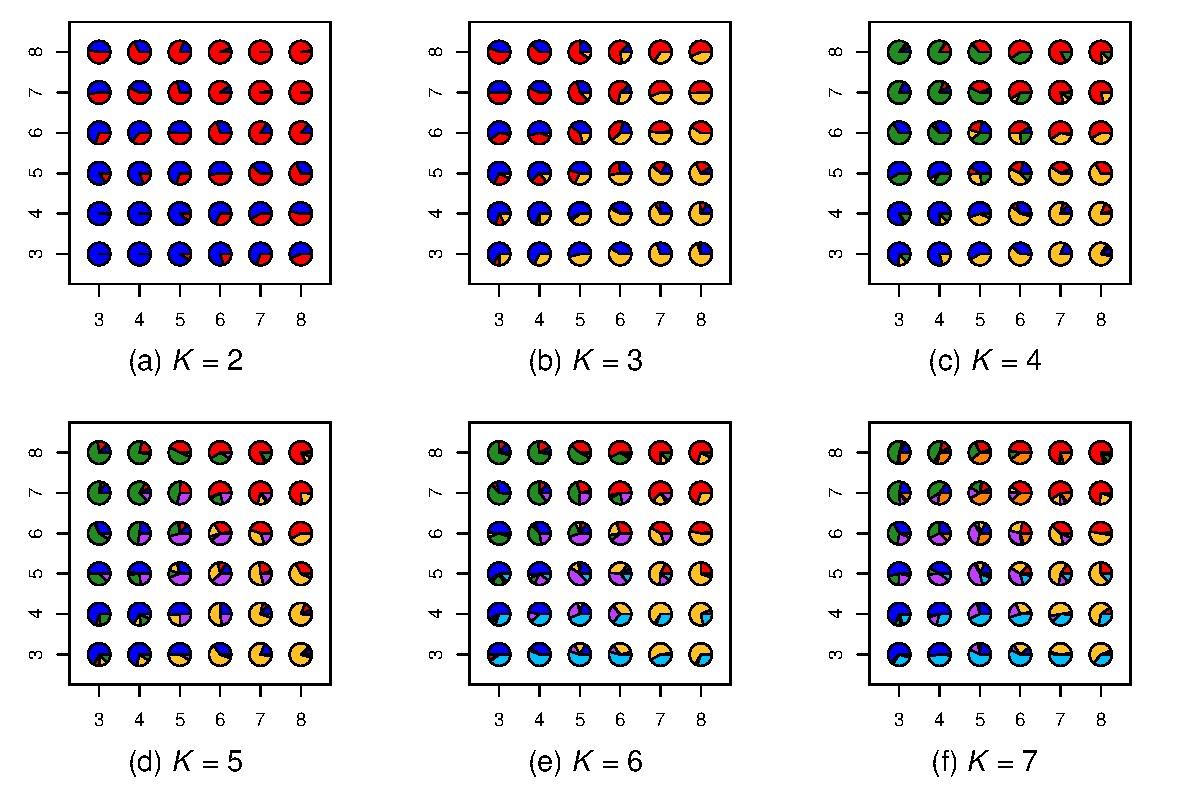
\includegraphics[width=\textwidth]{figs/sims/simK1_nsp_pies.pdf}}
	\caption{
	Map of admixture proportions estimated using a nonspatial model for $K=2$ through 7.
	The data were simulated using one layer with nearest-neighbor symmetric migration between demes.
    }\label{simK1_nsp_pies}
\end{figure}
\clearpage

\begin{figure}
	\centering
		{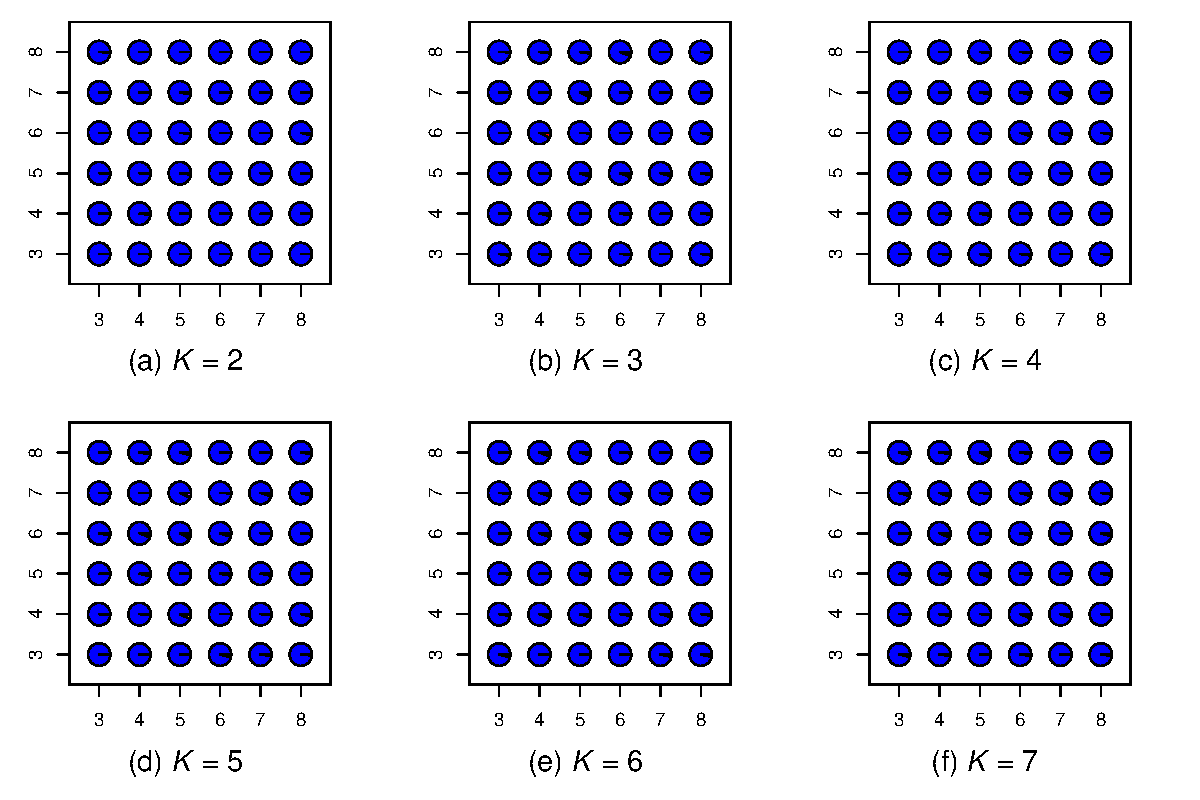
\includegraphics[width=\textwidth]{figs/sims/simK1_sp_pies.pdf}}
	\caption{
	Map of admixture proportions estimated using a spatial model for $K=2$ through 7.
	The data were simulated using one layer with nearest-neighbor symmetric migration between demes.
    }\label{simK1_sp_pies}
\end{figure}
\clearpage

\begin{figure}
	\centering
		{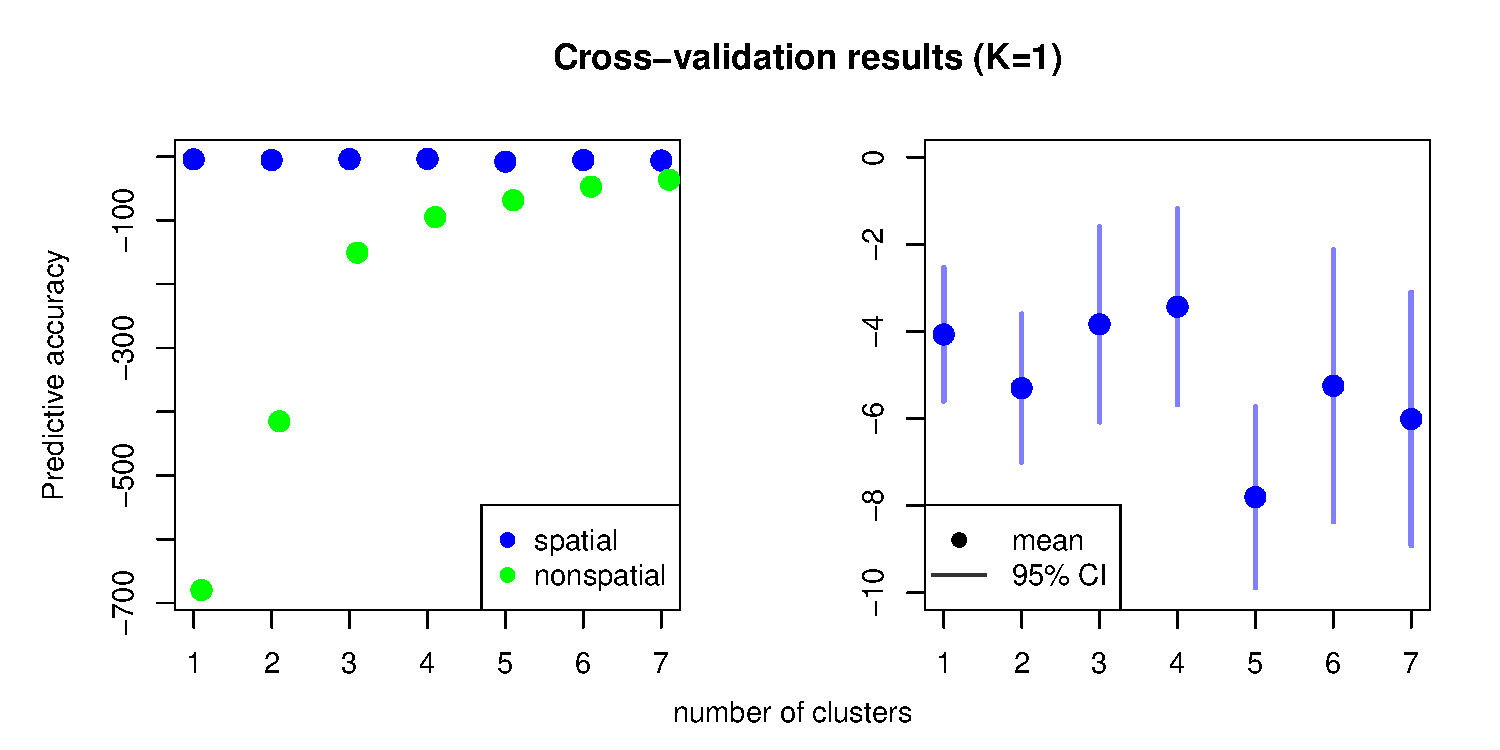
\includegraphics[width=\textwidth]{figs/sims/simK1_std_xval.pdf}}
		\caption{
			Cross-validation results for data simulated under $K=1$,
			comparing the spatial and nonspatial \texttt{conStruct} models run with $K=1$ through 7.  
			The right panel zooms in on just the spatial cross-validation results.
		}\label{simK1_xval}
\end{figure}
\clearpage

\begin{figure}
	\centering
		{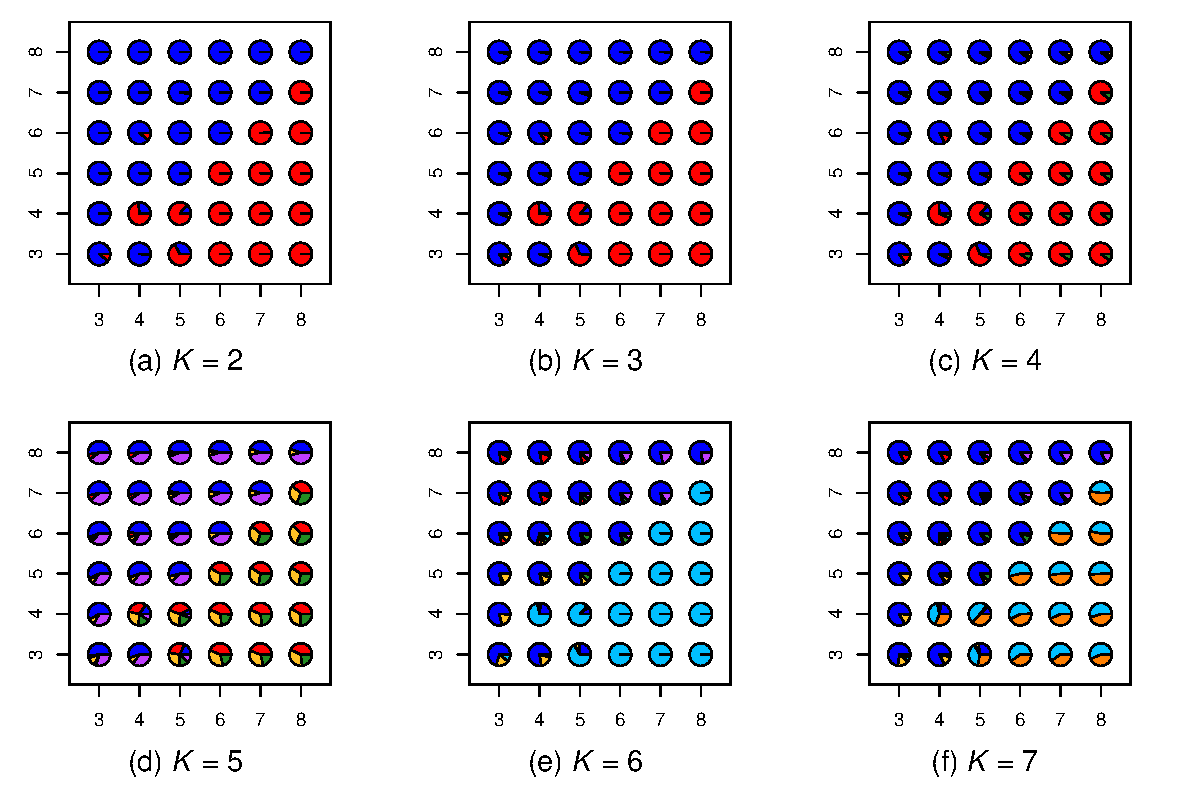
\includegraphics[width=\textwidth]{figs/sims/simK2_nsp_pies.pdf}}
	\caption{
	Map of admixture proportions estimated using a nonspatial model for $K=2$ through 7.
	The data were simulated using two layers with nearest-neighbor symmetric migration between demes.
    }\label{simK2_nsp_pies}
\end{figure}
\clearpage

\begin{figure}
	\centering
		{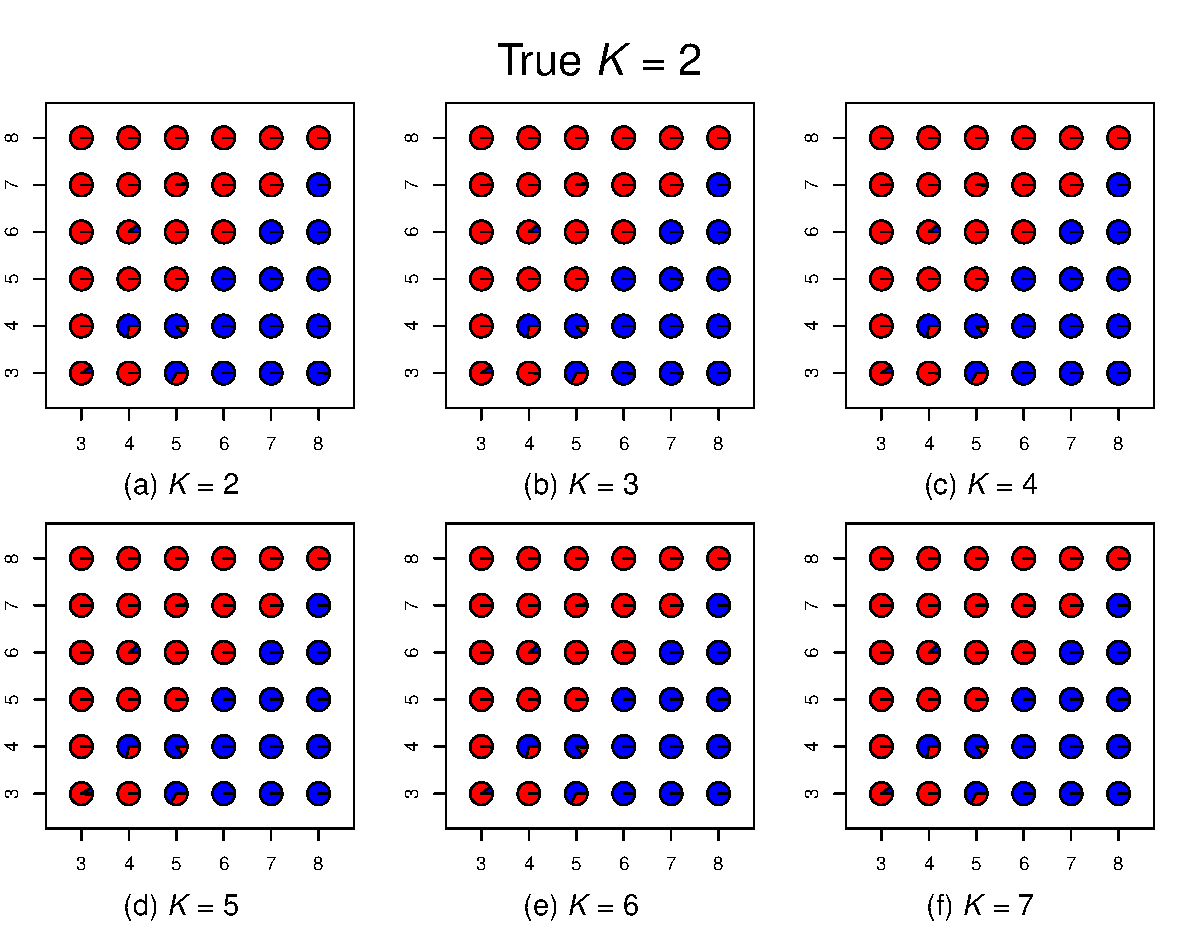
\includegraphics[width=\textwidth]{figs/sims/simK2_sp_pies.pdf}}
	\caption{
	Map of admixture proportions estimated using a spatial model for $K=2$ through 7.
	The data were simulated using two layers with nearest-neighbor symmetric migration between demes.
    }\label{simK2_sp_pies}
\end{figure}
\clearpage

\begin{figure}
	\centering
		{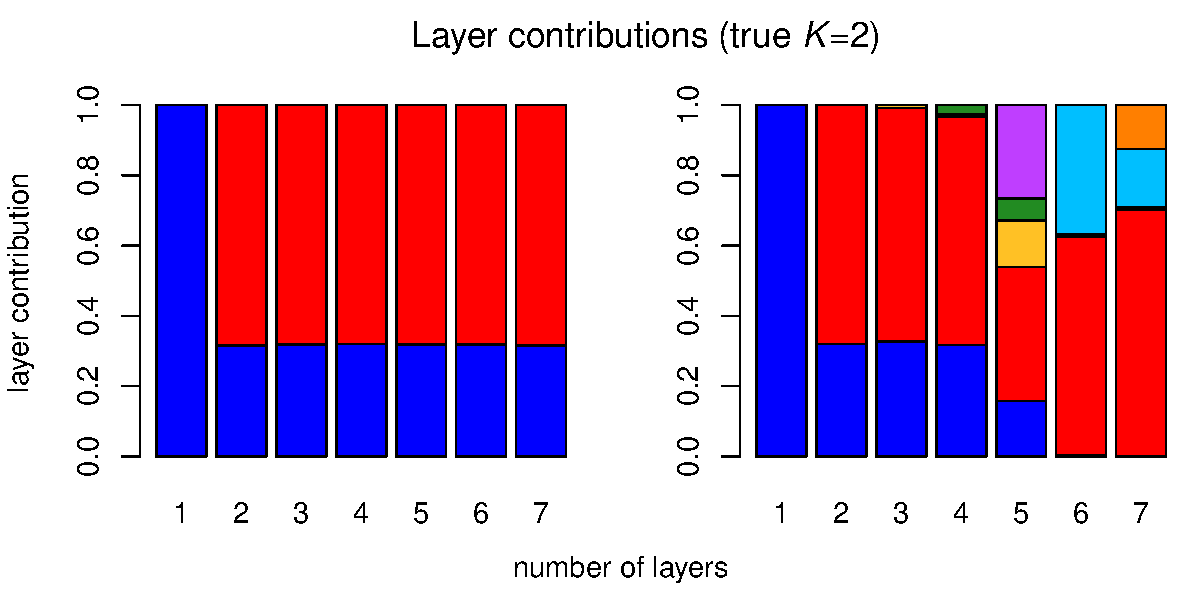
\includegraphics[width=\textwidth]{figs/sims/simK2_laycon_barplots.pdf}}
		\caption{
			Layer/cluster contributions (i.e., how much total covariance is contributed by each layer/cluster), 
			for all layers estimated in runs using $K = 1$ through 7 
			for the spatial model (left), 
			and for all clusters using the nonspatial model (right).
			Data were simulated using $K=2$.
			For each value of $K$ along the x-axis, there are an equal number of contributions plotted.
		}\label{simK2_laycon}
\end{figure}
\clearpage

\begin{figure}
	\centering
		{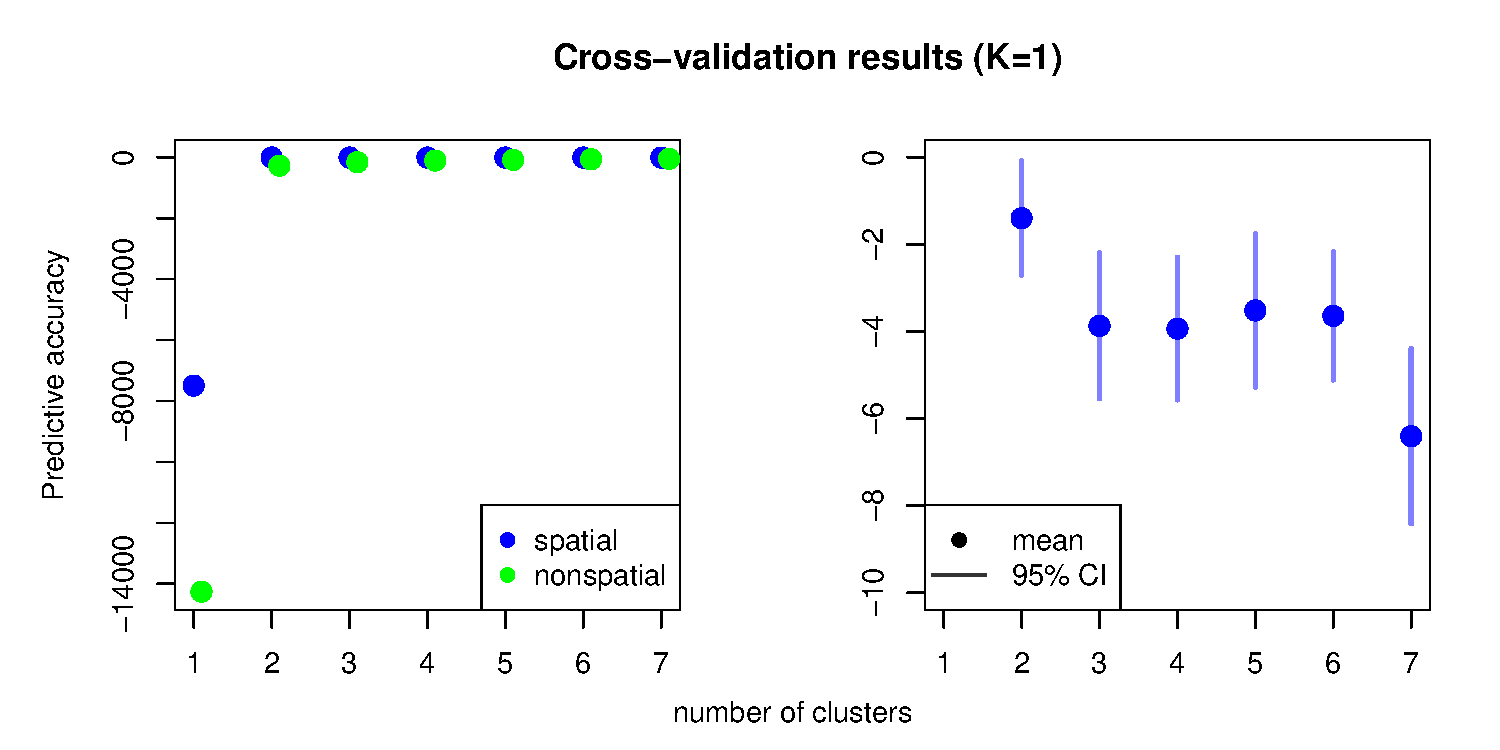
\includegraphics[width=\textwidth]{figs/sims/simK2_std_xval.pdf}}
		\caption{
			Cross-validation results for data simulated under $K=2$,
			comparing the spatial and nonspatial \texttt{conStruct} models run with $K=1$ through 7.  
			The right panel zooms in on just the spatial cross-validation results.
		}\label{simK2_xval}
\end{figure}
\clearpage

\begin{figure}
	\centering
		{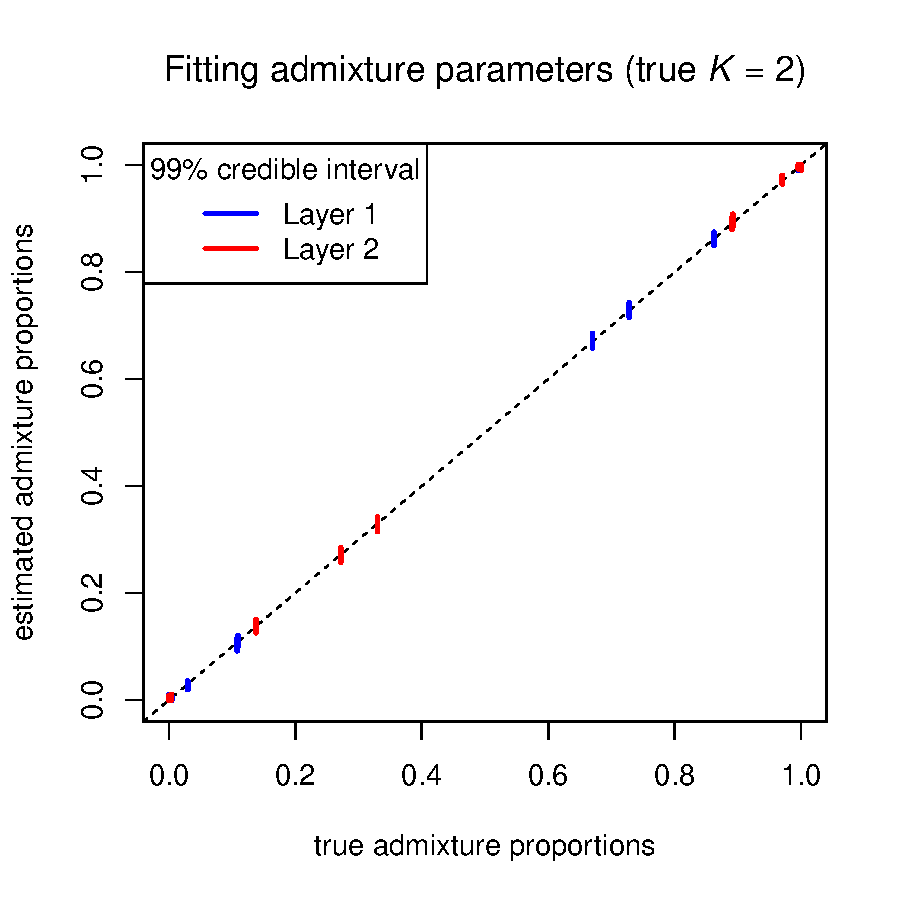
\includegraphics[width=\textwidth]{figs/sims/simK2_adprop_fit.pdf}}
		\caption{
			Plot of \texttt{conStruct} ability to correctly estimate admixture proportions on simulated data.
			Results are from an analysis with a spatial model using $K=2$.
		}\label{simK2_adprop_fit}
\end{figure}
\clearpage

\begin{figure}
	\centering
		{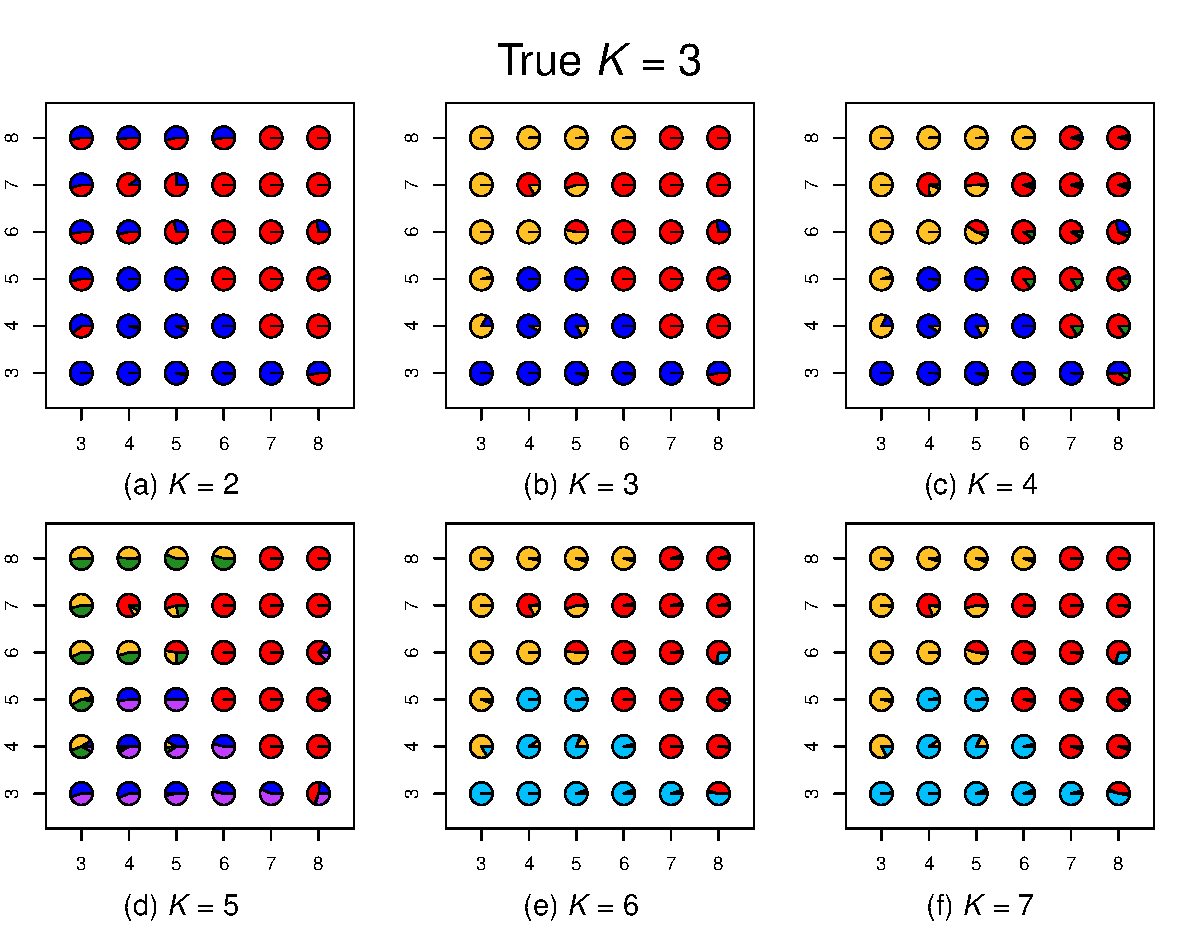
\includegraphics[width=\textwidth]{figs/sims/simK3_nsp_pies.pdf}}
	\caption{
	Map of admixture proportions estimated using a nonspatial model for $K=2$ through 7.
	The data were simulated using three layers with nearest-neighbor symmetric migration between demes.
    }\label{simK3_nsp_pies}
\end{figure}
\clearpage

\begin{figure}
	\centering
		{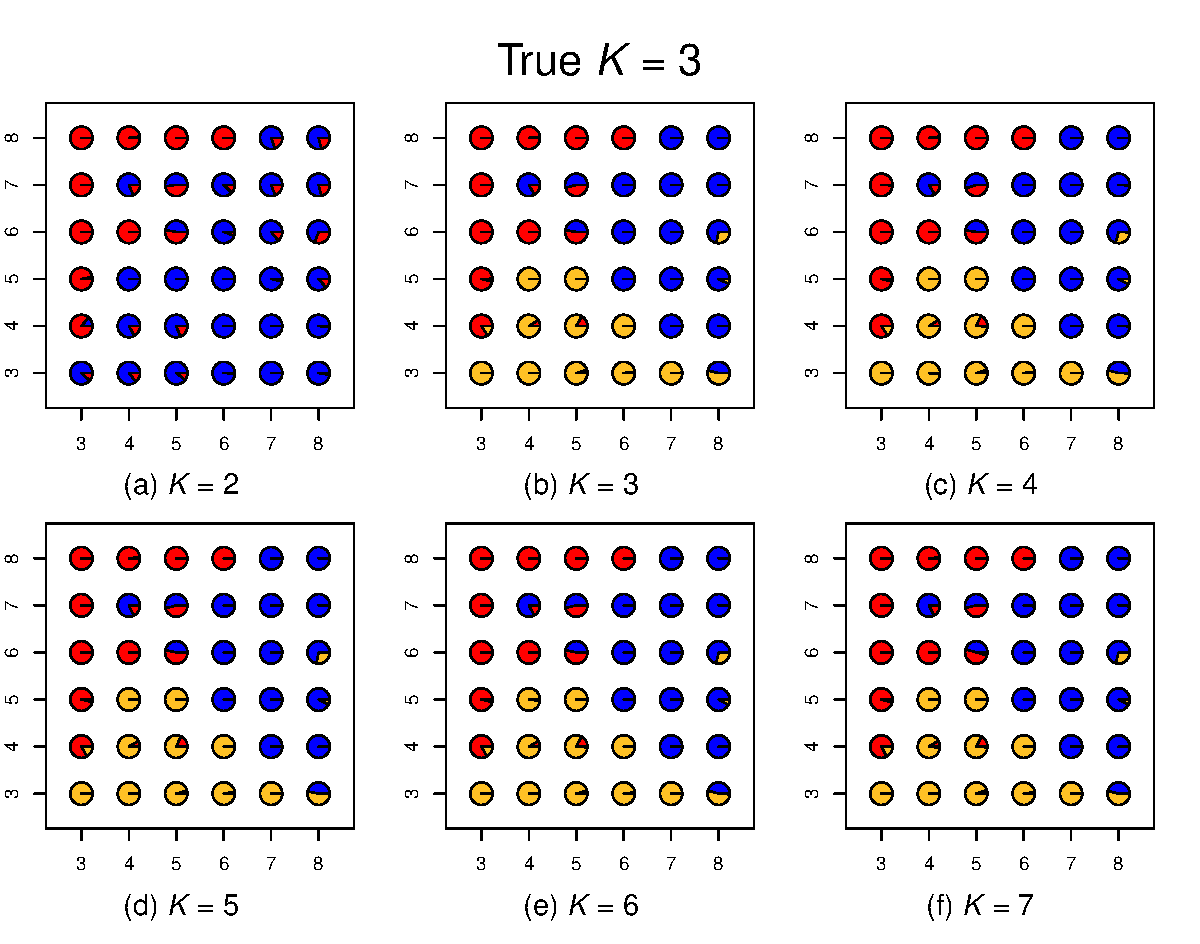
\includegraphics[width=\textwidth]{figs/sims/simK3_sp_pies.pdf}}
	\caption{
	Map of admixture proportions estimated using a spatial model for $K=2$ through 7.
	The data were simulated using three layers with nearest-neighbor symmetric migration between demes.
    }\label{simK3_sp_pies}
\end{figure}
\clearpage

\begin{figure}
	\centering
		{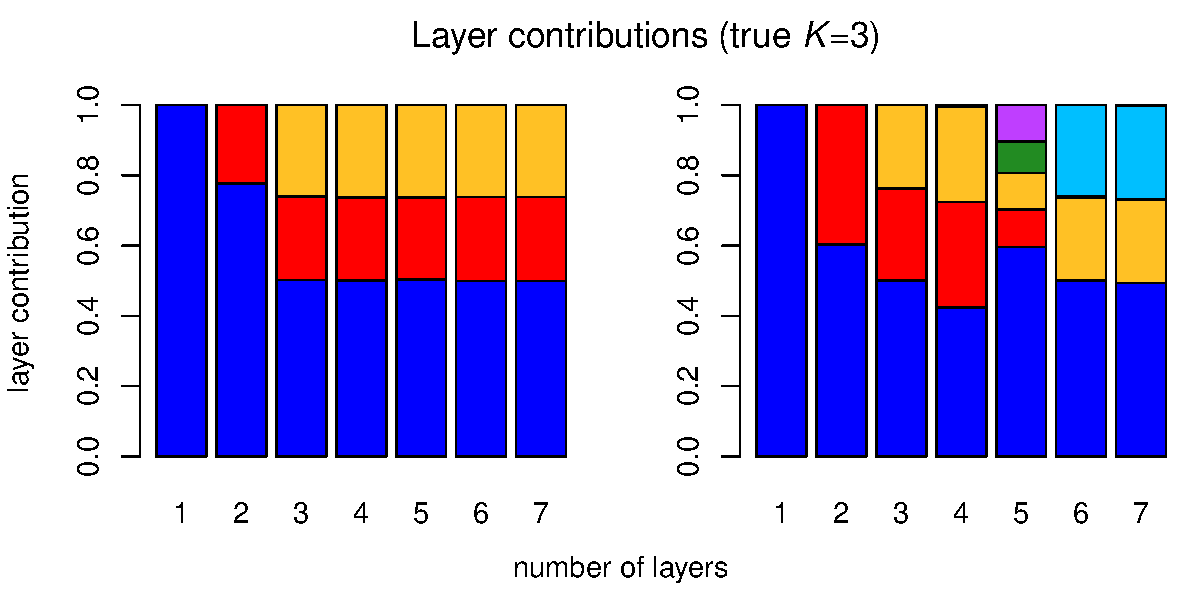
\includegraphics[width=\textwidth]{figs/sims/simK3_laycon_barplots.pdf}}
		\caption{
			Layer/cluster contributions (i.e., how much total covariance is contributed by each layer/cluster), 
			for all layers estimated in runs using $K = 1$ through 7 
			for the spatial model (left), 
			and for all clusters using the nonspatial model (right).
			Data were simulated using $K=3$.
			For each value of $K$ along the x-axis, there are an equal number of contributions plotted.
		}\label{simK3_laycon}
\end{figure}
\clearpage

\begin{figure}
	\centering
		{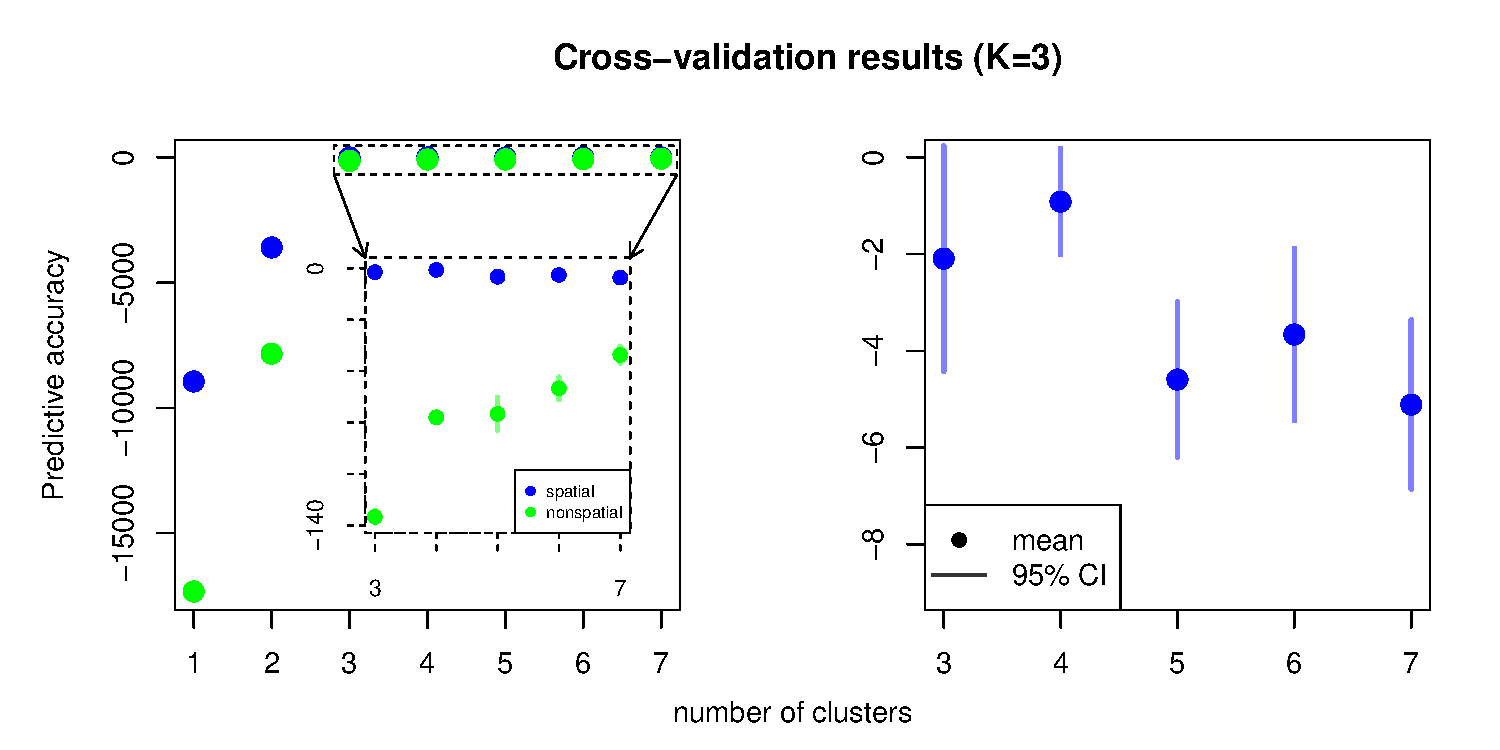
\includegraphics[width=\textwidth]{figs/sims/simK3_std_xval.pdf}}
		\caption{
			Cross-validation results for data simulated under $K=3$,
			comparing the spatial and nonspatial \texttt{conStruct} models run with $K=1$ through 7.  
			The right panel zooms in on just the spatial cross-validation results.
		}\label{simK3_xval}
\end{figure}
\clearpage

\begin{figure}
	\centering
		{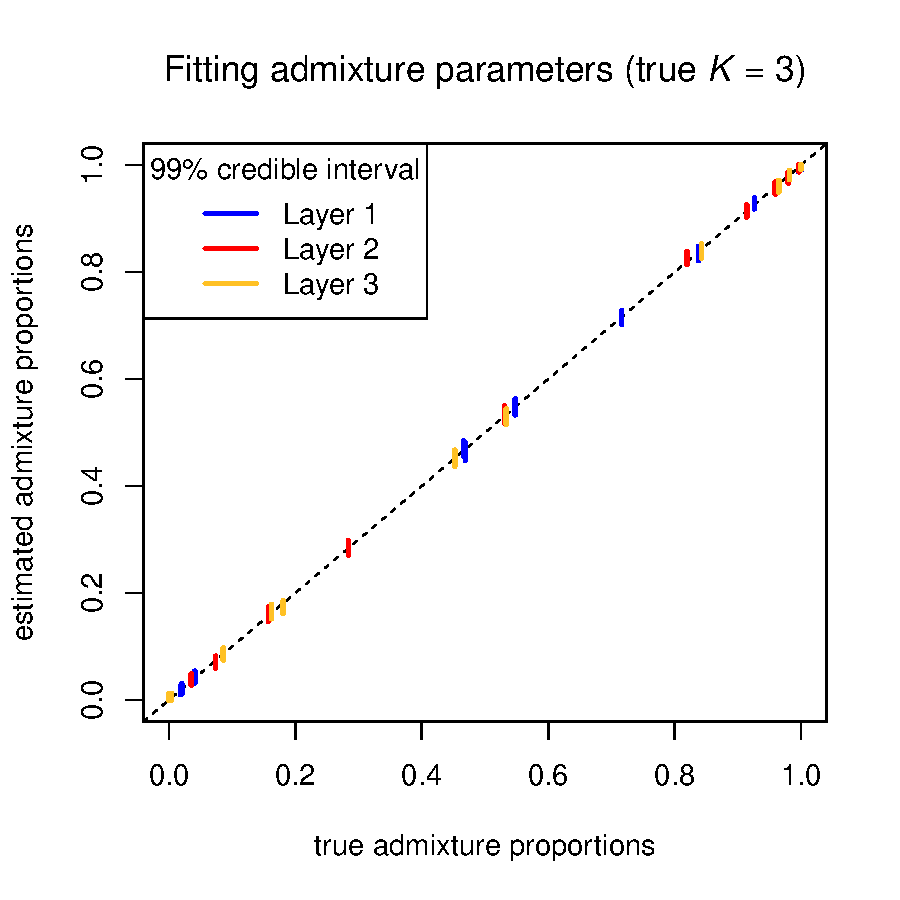
\includegraphics[width=\textwidth]{figs/sims/simK3_adprop_fit.pdf}}
		\caption{
			Plot of \texttt{conStruct} ability to correctly estimate admixture proportions on simulated data.
			Results are from an analysis with a spatial model using $K=3$.
		}\label{simK3_adprop_fit}
\end{figure}
\clearpage

\begin{figure}
	\centering
		{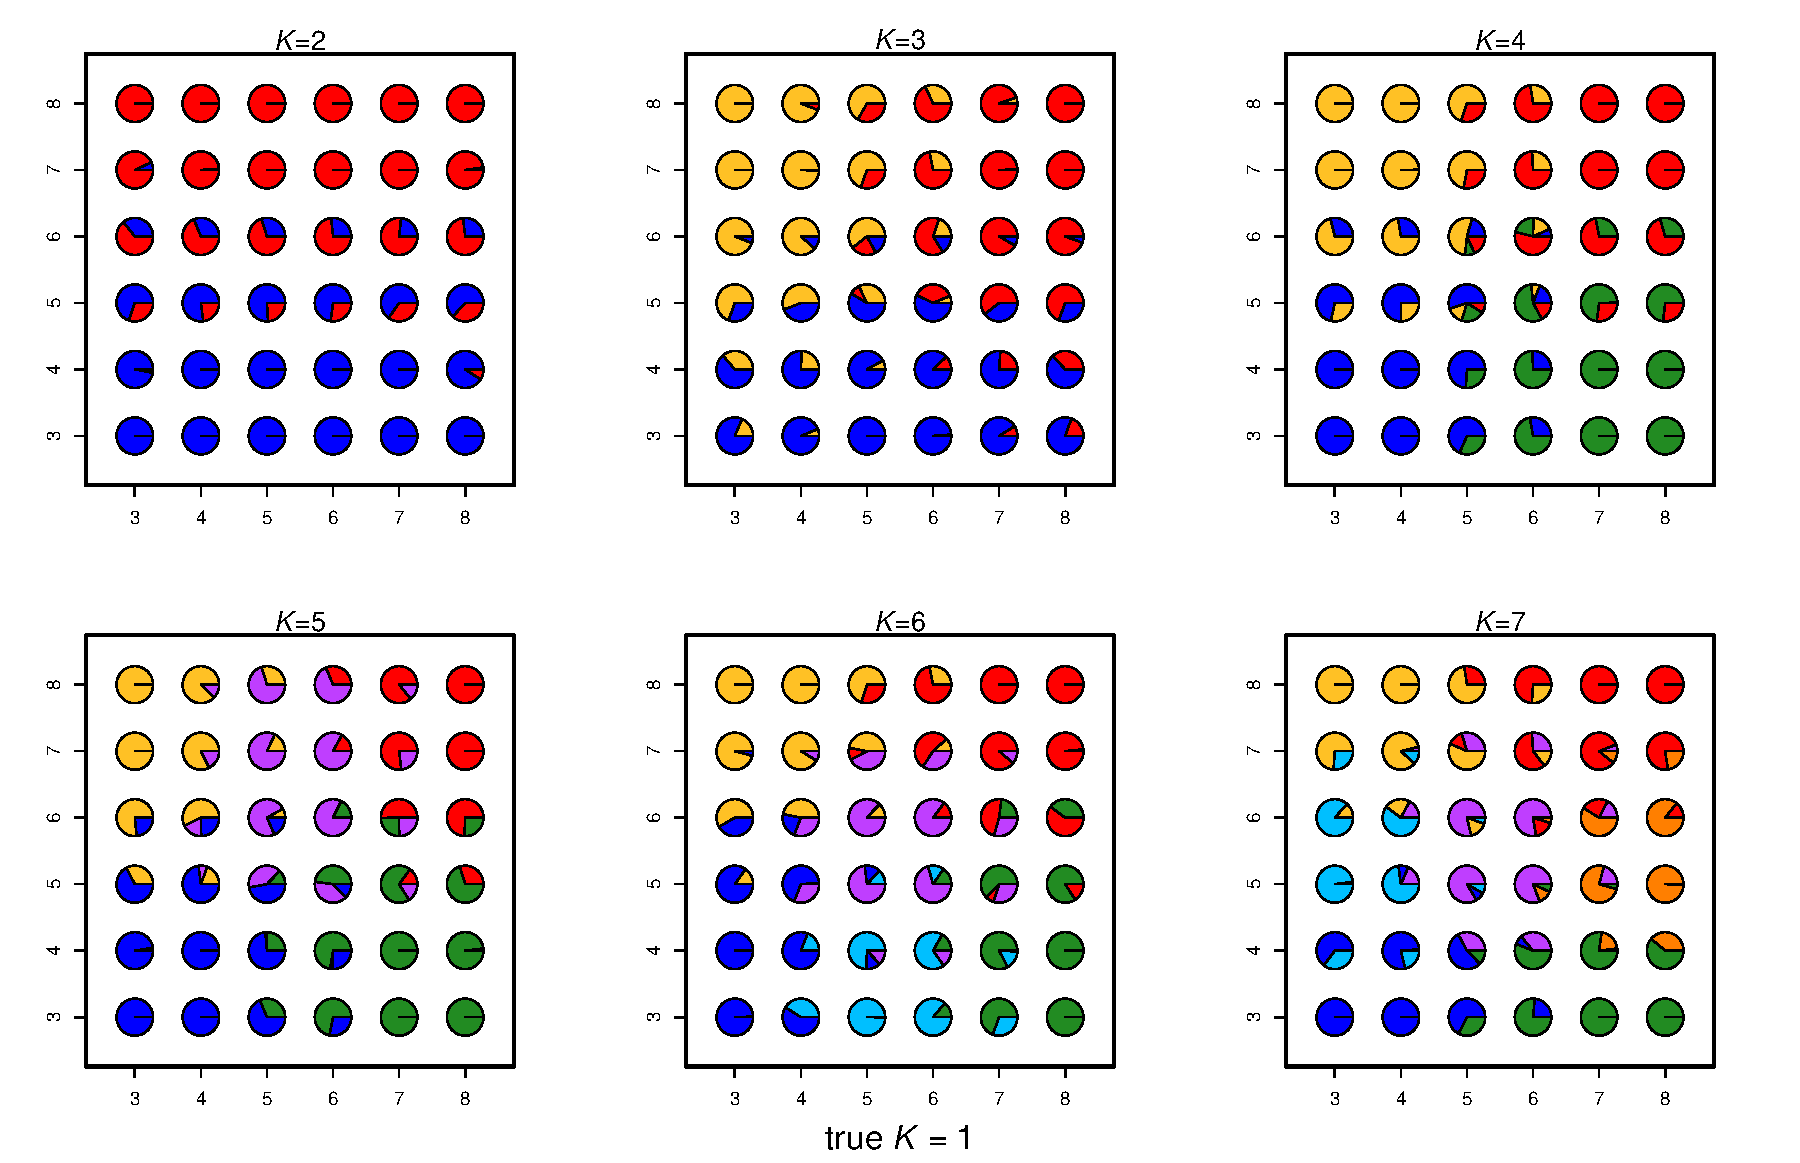
\includegraphics[width=\textwidth]{figs/admixture/admixture_simK1_pies.pdf}}
	\caption{
	Map of admixture proportions estimated using ADMIXTURE \cite{ADMIXTURE} for $K=2$ through 7.
	The data were simulated using one layer with nearest-neighbor symmetric migration between demes.
	The model with the lowest cross-validation error (i.e., the preferred model) is indicated with an asterisk.
    }\label{admix_simK1}
\end{figure}
\clearpage

\begin{figure}
	\centering
		{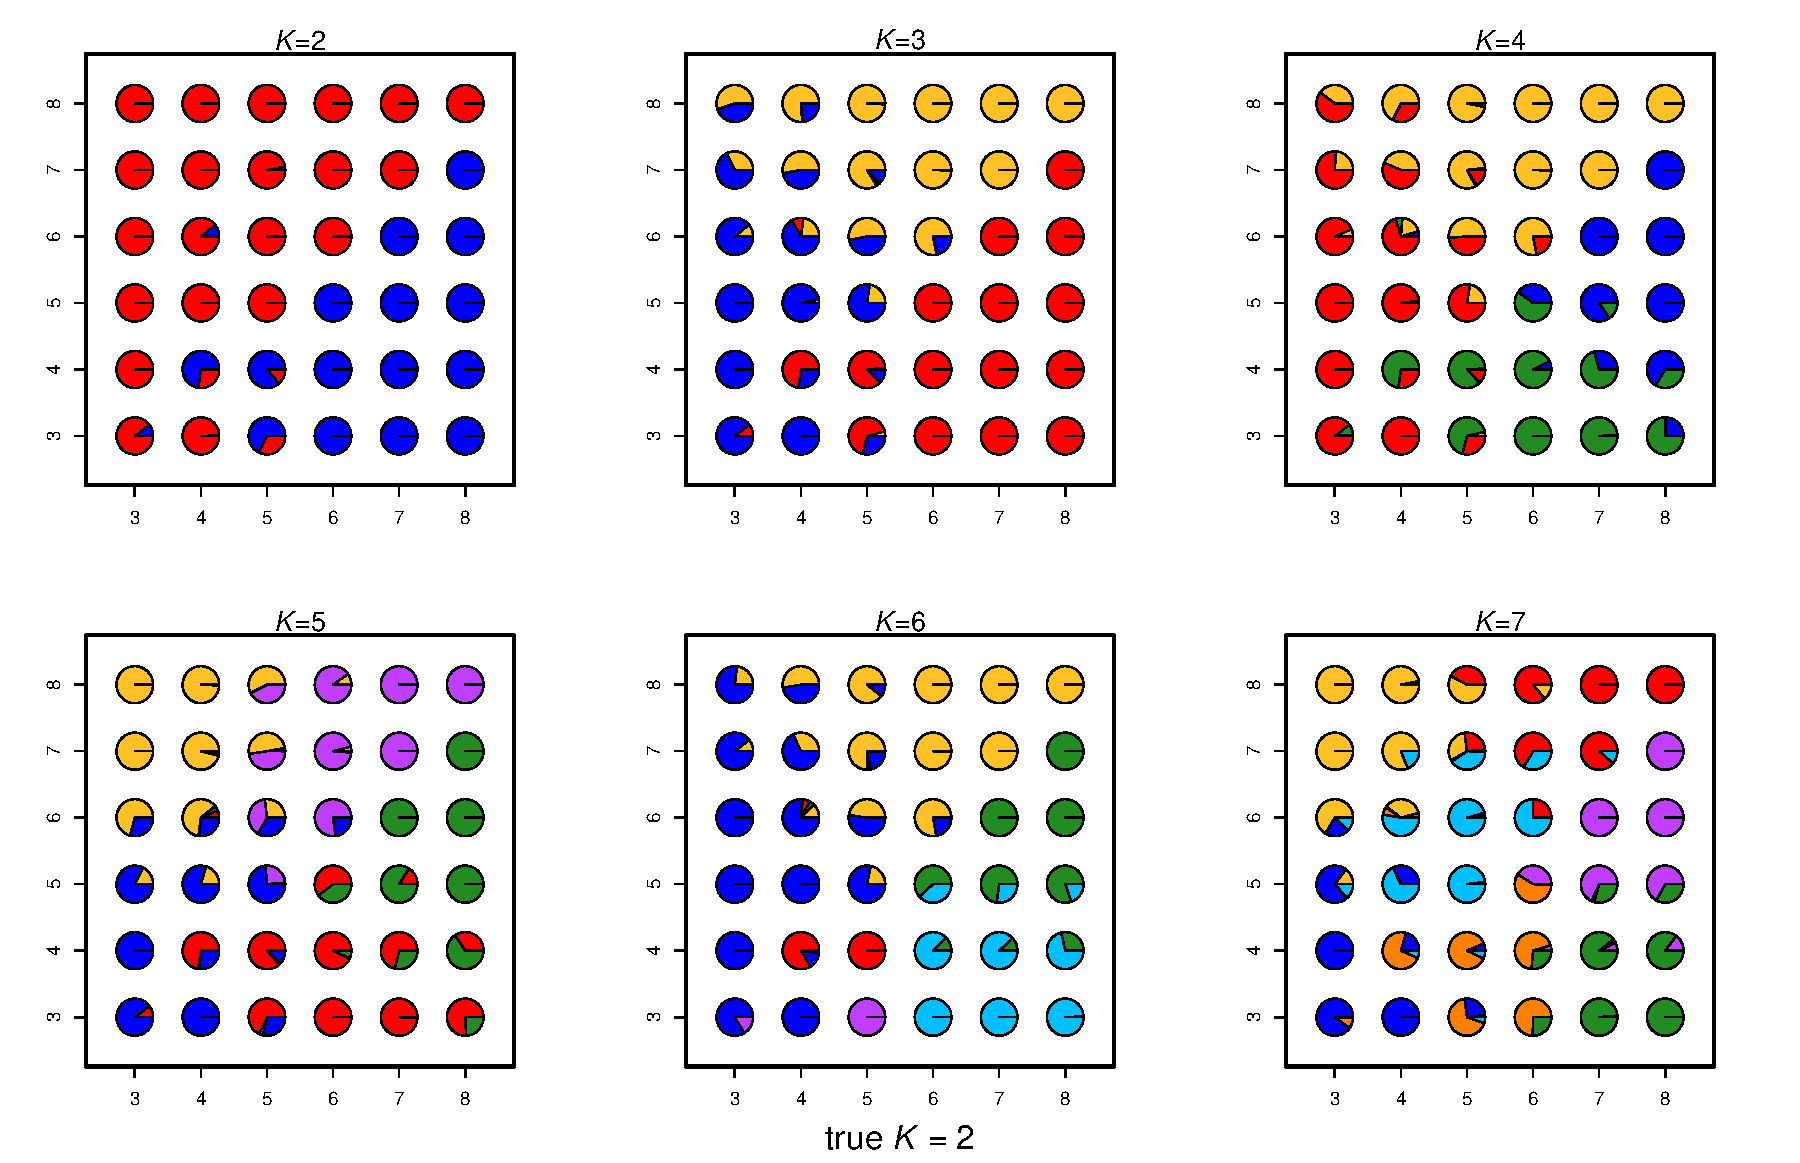
\includegraphics[width=\textwidth]{figs/admixture/admixture_simK2_pies.pdf}}
	\caption{
	Map of admixture proportions estimated using ADMIXTURE \cite{ADMIXTURE} for $K=2$ through 7.
	The data were simulated using two layers with nearest-neighbor symmetric migration between demes.
	The model with the lowest cross-validation error (i.e., the preferred model) is indicated with an asterisk.
    }\label{admix_simK2}
\end{figure}
\clearpage

\begin{figure}
	\centering
		{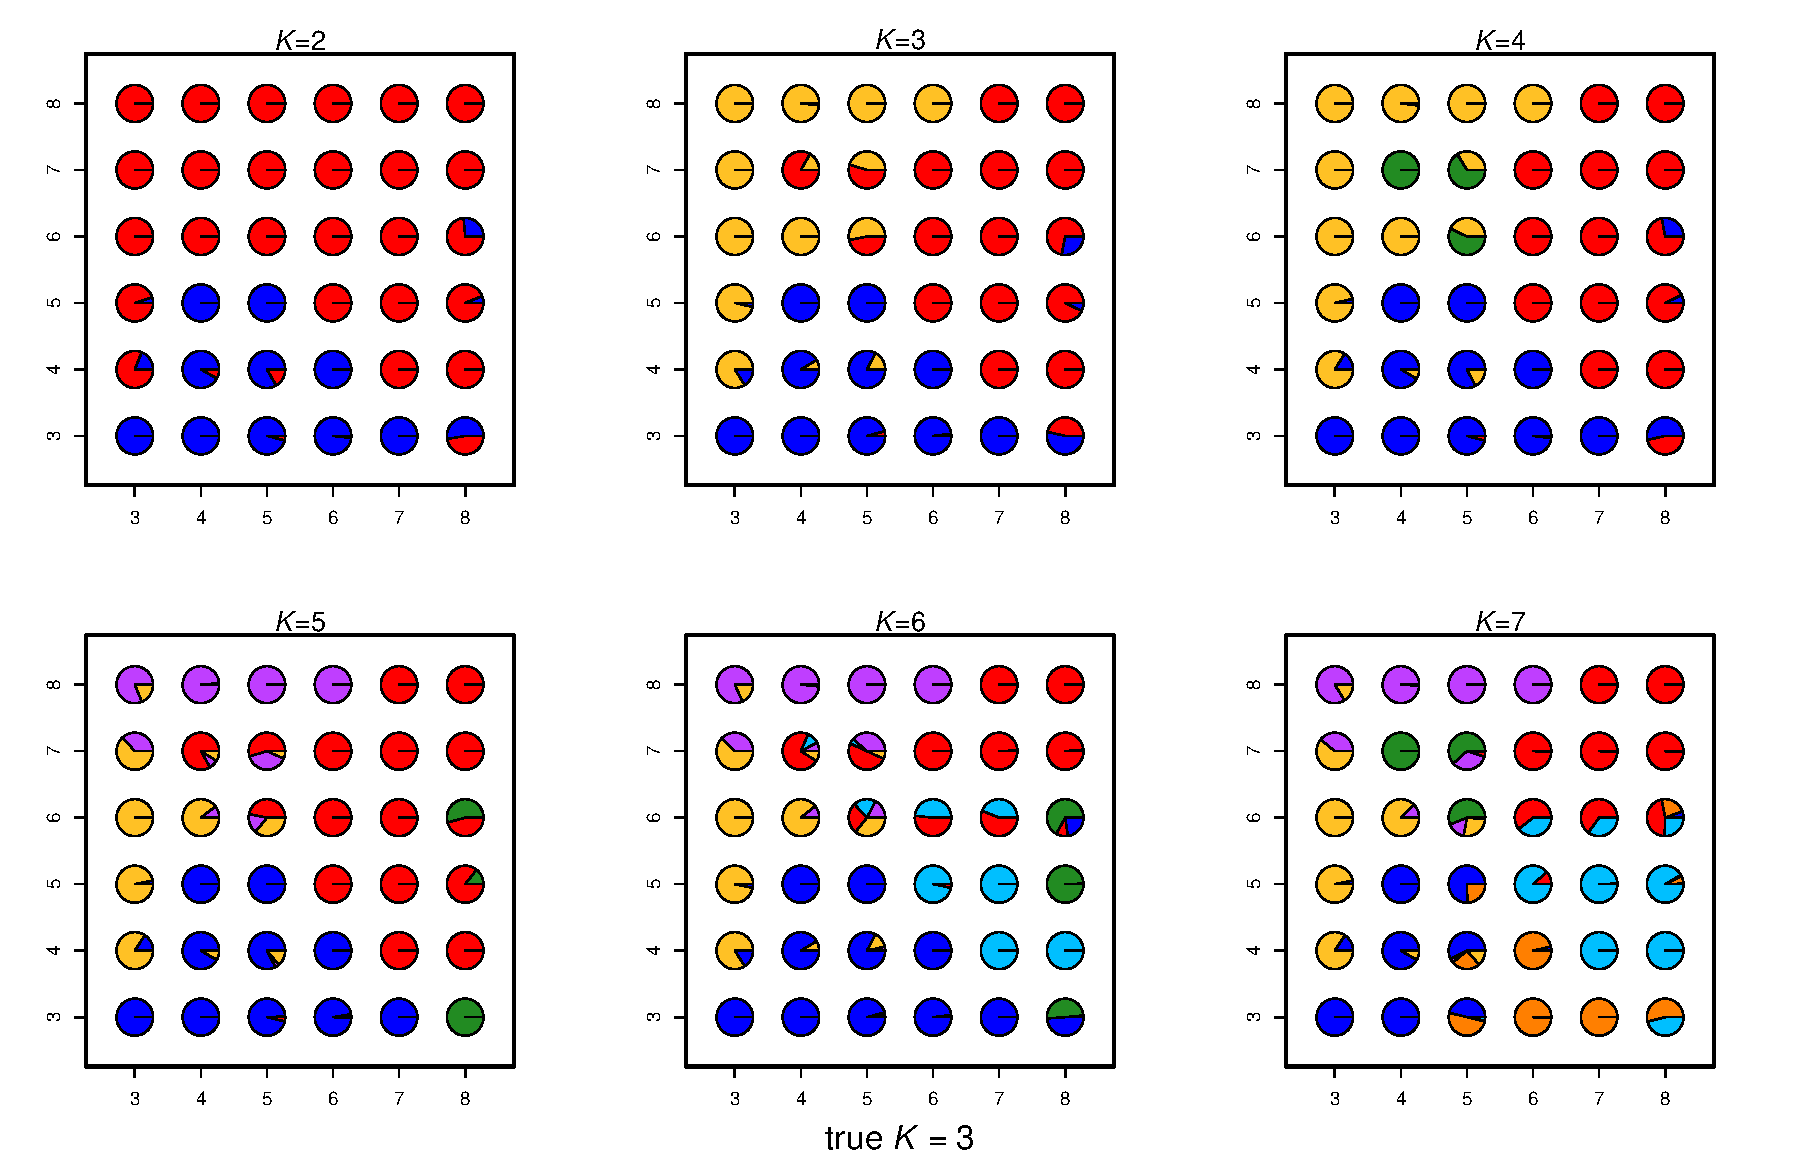
\includegraphics[width=\textwidth]{figs/admixture/admixture_simK3_pies.pdf}}
	\caption{
	Map of admixture proportions estimated using ADMIXTURE \cite{ADMIXTURE} for $K=2$ through 7.
	The data were simulated using three layers with nearest-neighbor symmetric migration between demes.
	The model with the lowest cross-validation error (i.e., the preferred model) is indicated with an asterisk.
    }\label{admix_simK3}
\end{figure}
\clearpage

\begin{figure}
	\centering
		{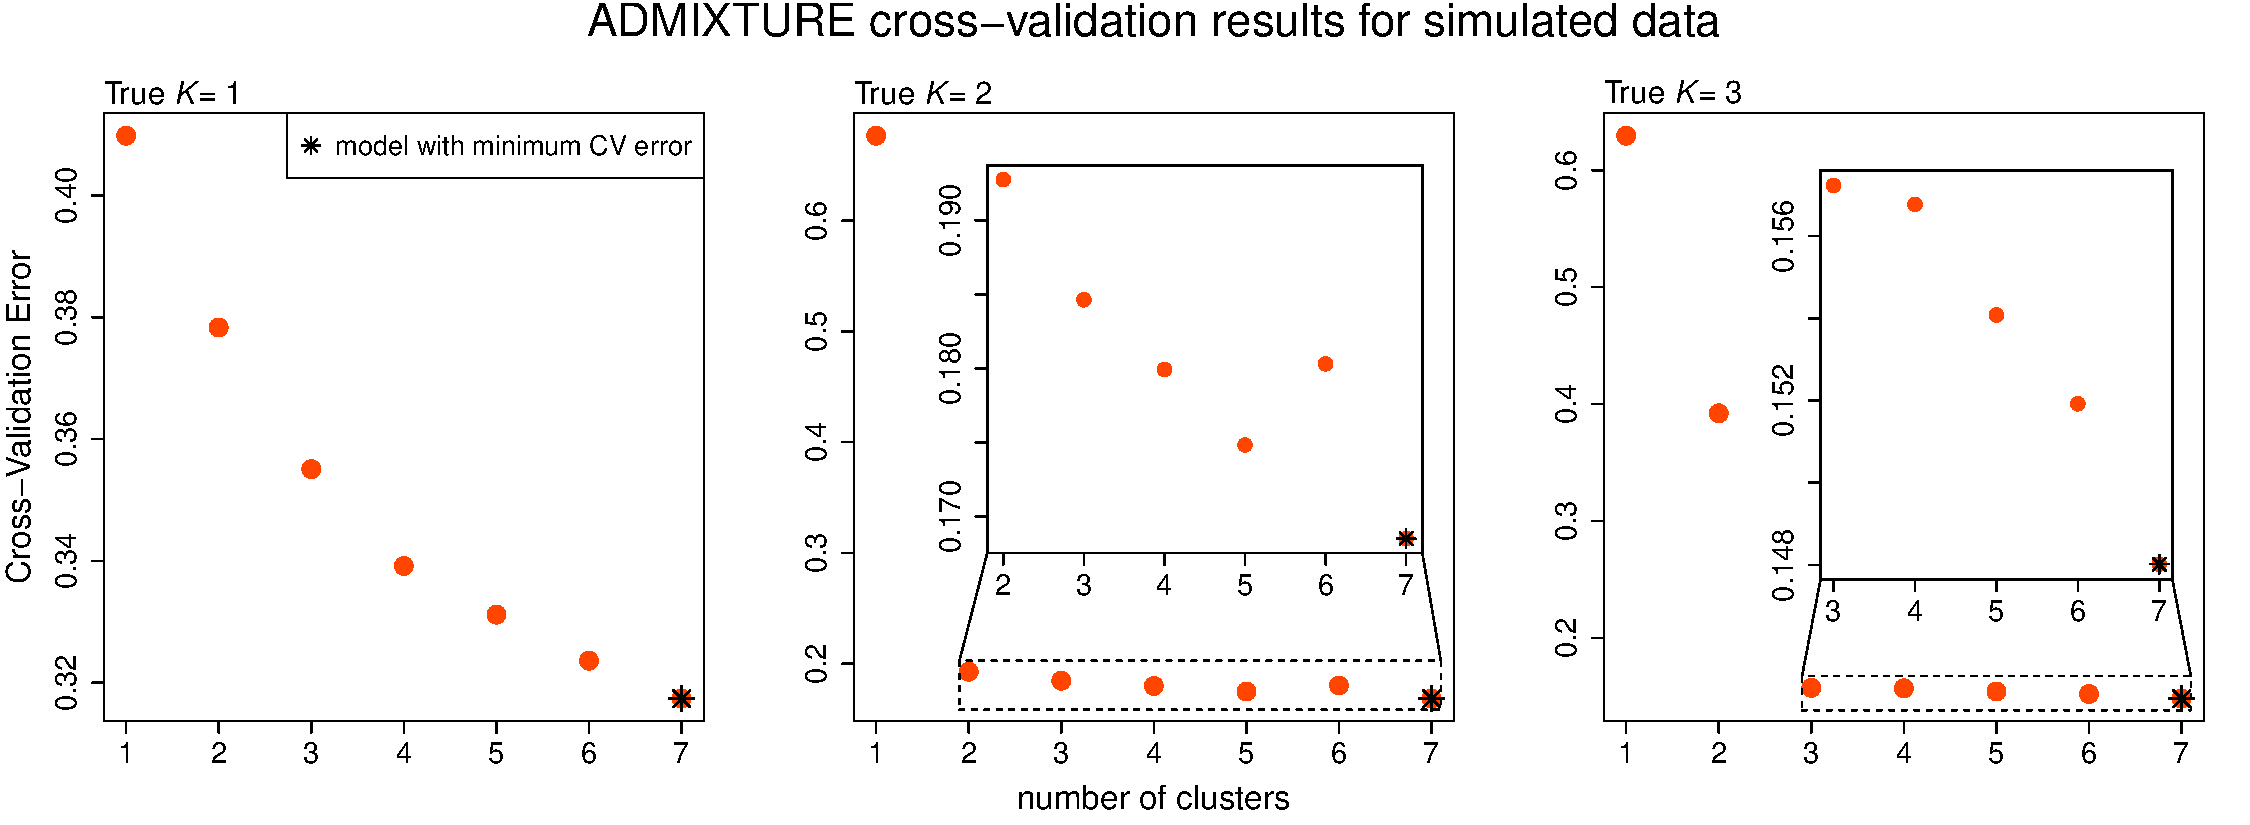
\includegraphics[width=\textwidth]{figs/admixture/sims_CVerror.pdf}}
	\caption{
	ADMIXTURE cross-validation results for data simulated under $K=1$, $K=2$, and $K=3$, 
	run with $K=1$ through 7 using 50 data ``folds" (\texttt{--cv=50}).  
	The inset plots zoom in on cross-validation results outlined in the dotted boxes.
	The preferred model (with the lowest cross-validation error) is highlighted with an asterisk.
    }\label{sim_admix_CVerrors}
\end{figure}
\clearpage

\begin{figure}
	\centering
		{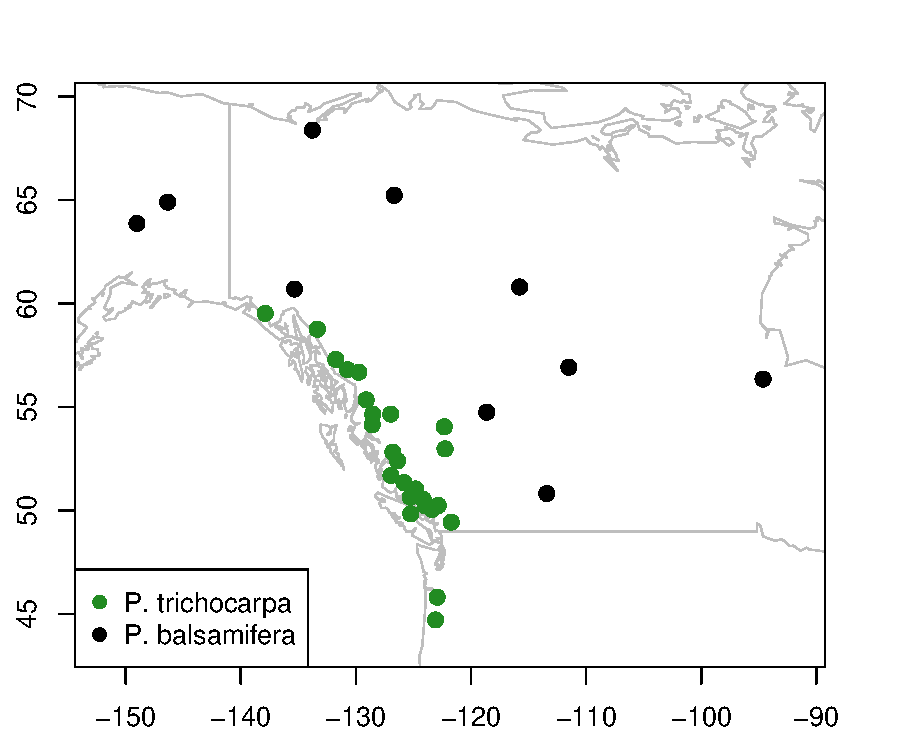
\includegraphics[width=\textwidth]{figs/populus/populus_sampling_map.pdf}}
	\caption{
	Map of the sampled \textit{Populus} populations included in the analysis.
	The color of the sampling location denotes the putative species.
    }\label{populus_map}
\end{figure}
\clearpage

\begin{figure}
	\centering
		{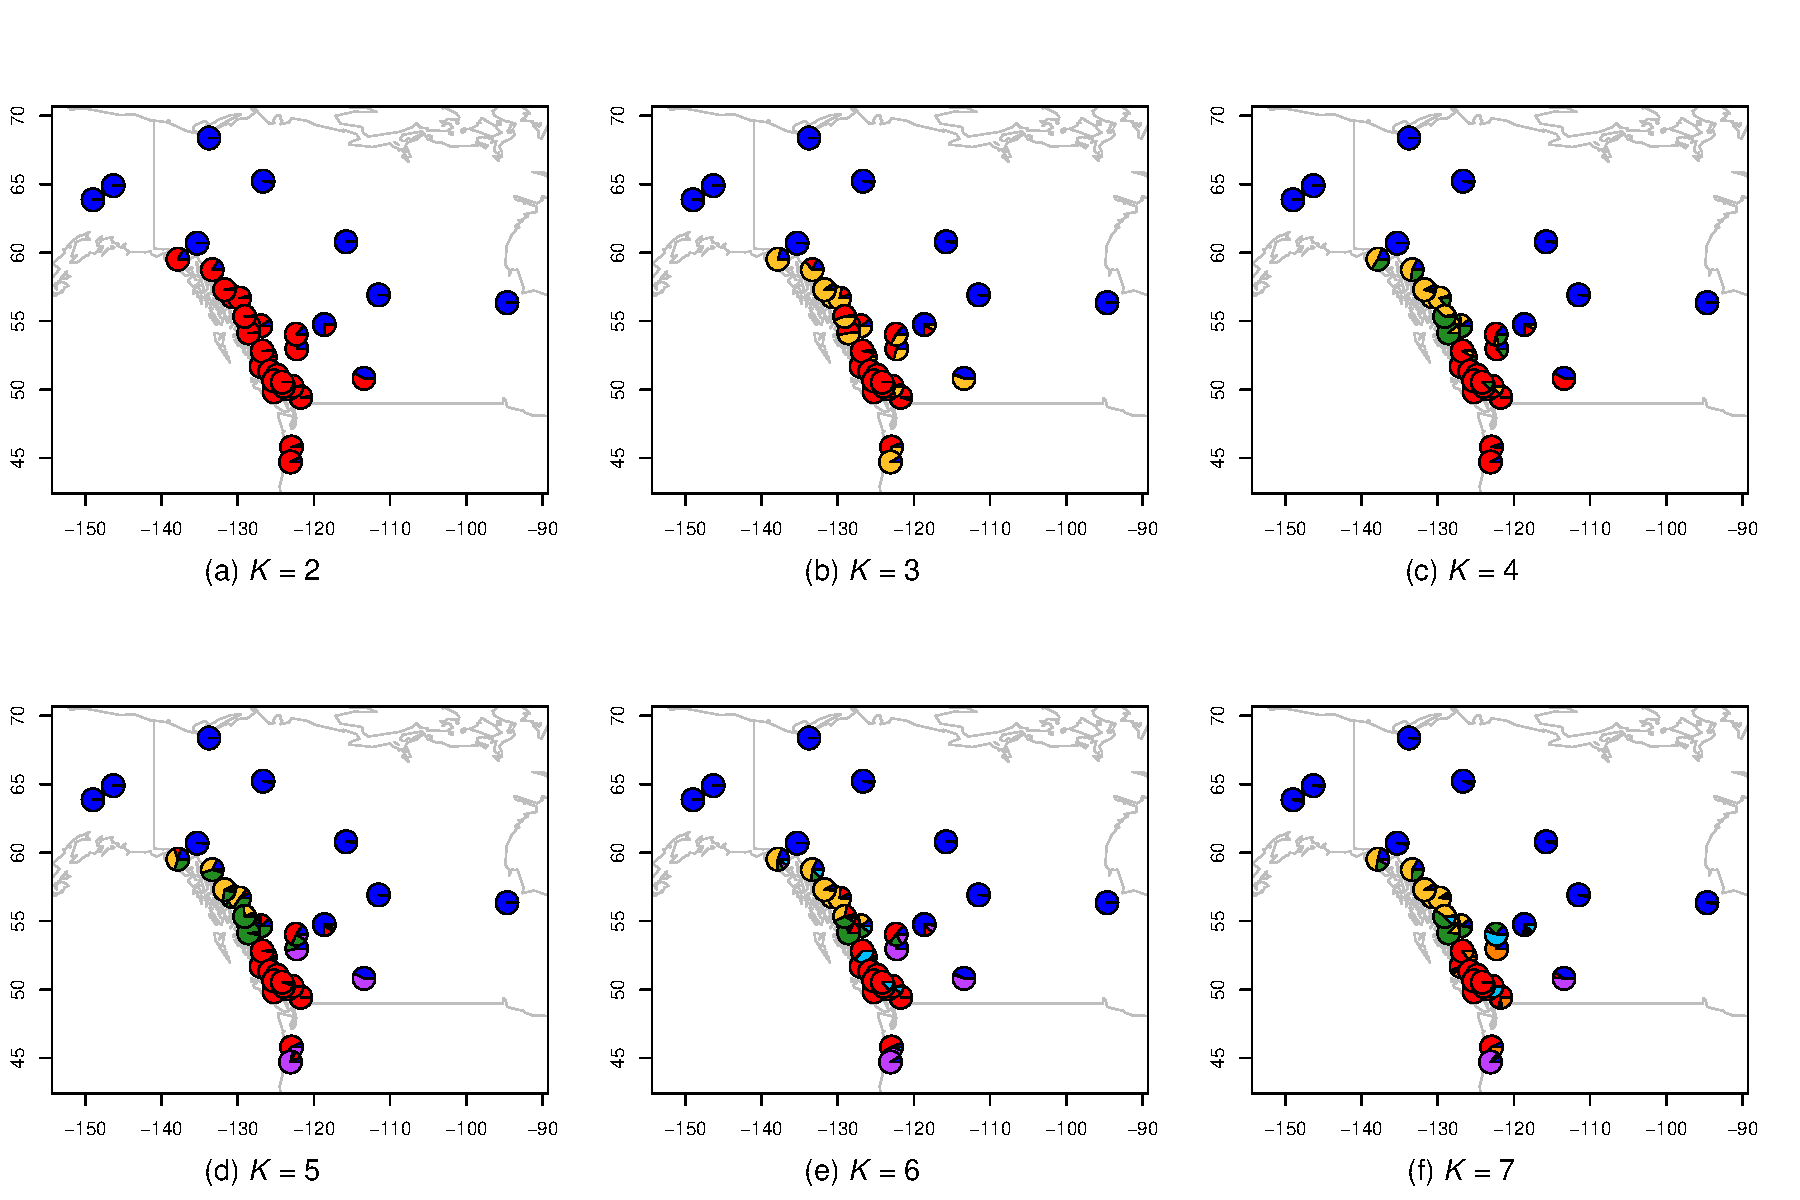
\includegraphics[width=\textwidth]{figs/populus/populus_sp_pies.pdf}}
	\caption{
	Maps of admixture proportions estimated for the \textit{Populus} dataset 
	using the spatial model for $K=2$ through 7.
    }\label{populus_sp_pies}
\end{figure}
\clearpage

\begin{figure}
	\centering
		{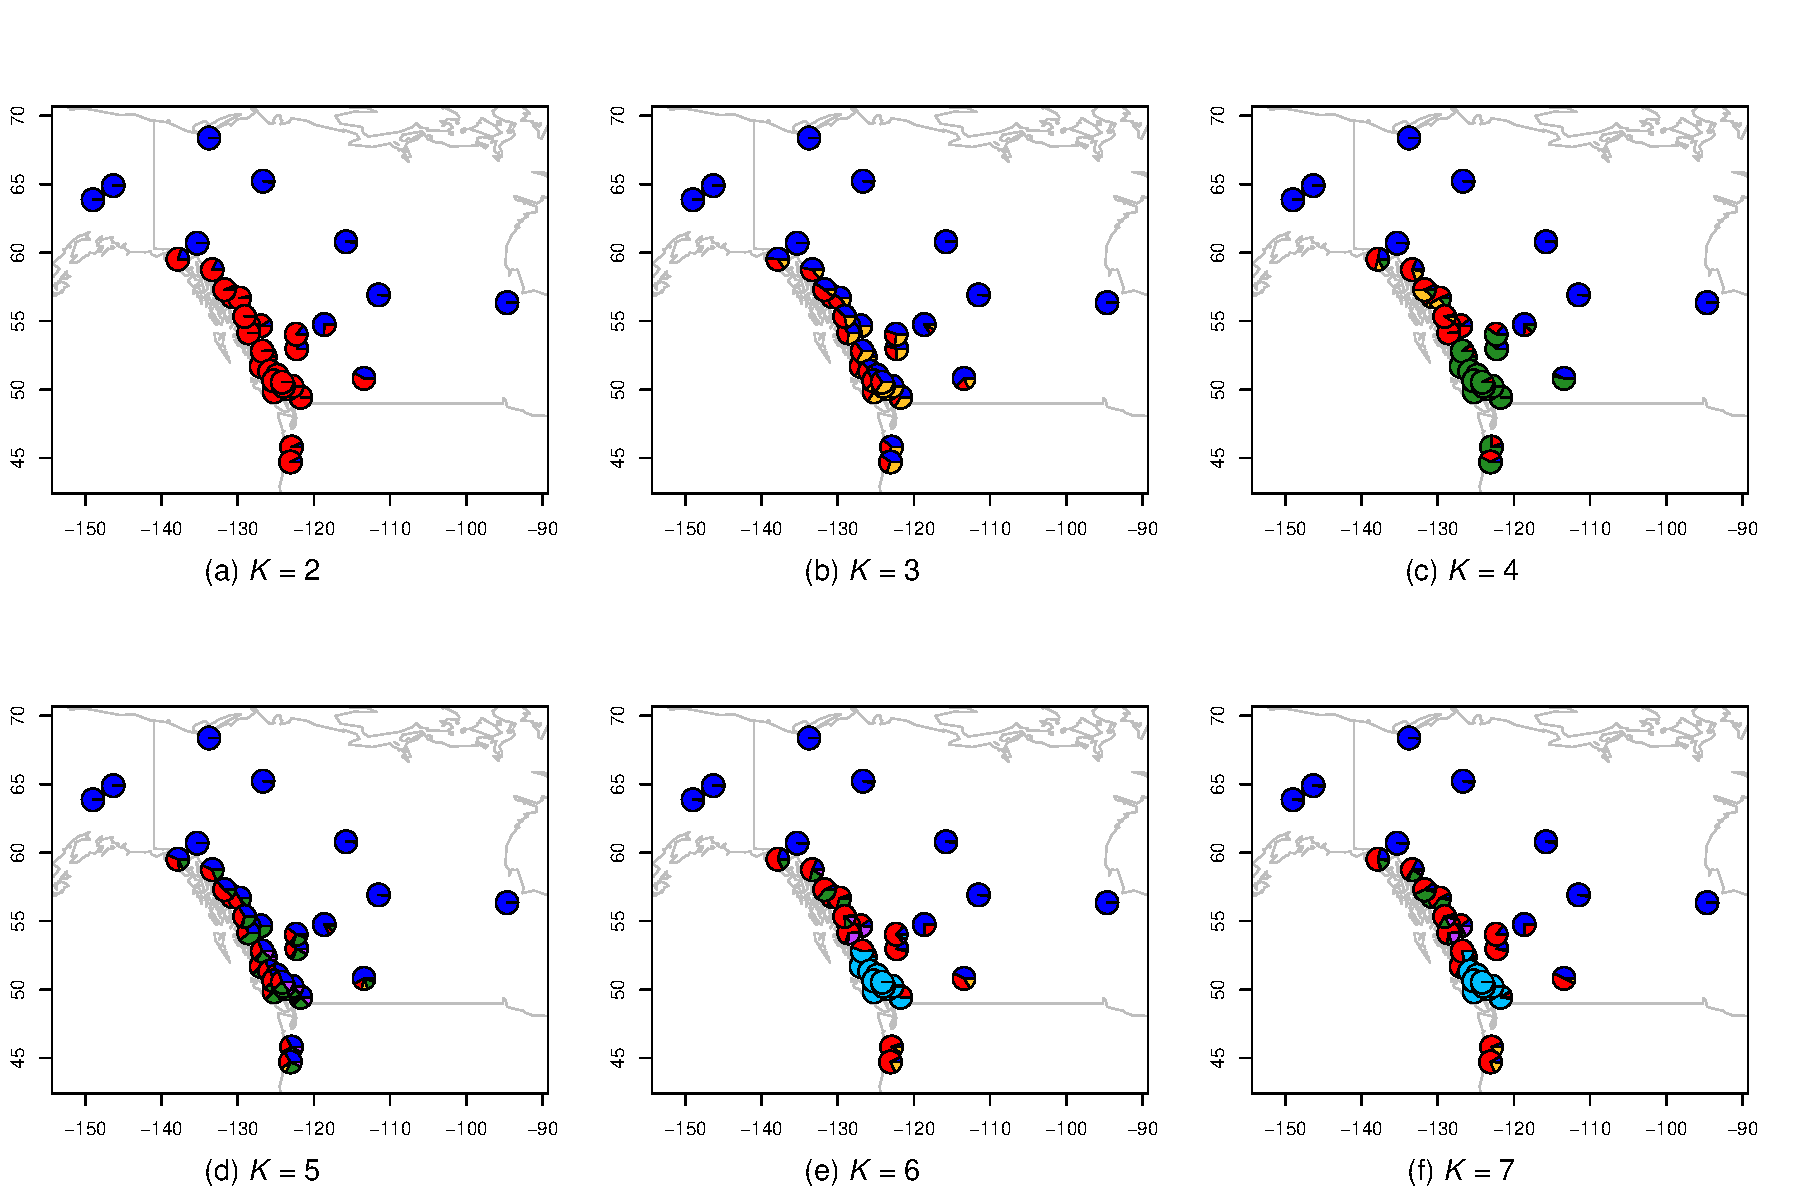
\includegraphics[width=\textwidth]{figs/populus/populus_nsp_pies.pdf}}
	\caption{
	Maps of admixture proportions estimated for the \textit{Populus} dataset 
	using the nonspatial model for $K=2$ through 7.
    }\label{populus_nsp_pies}
\end{figure}
\clearpage

\begin{figure}
	\centering
		{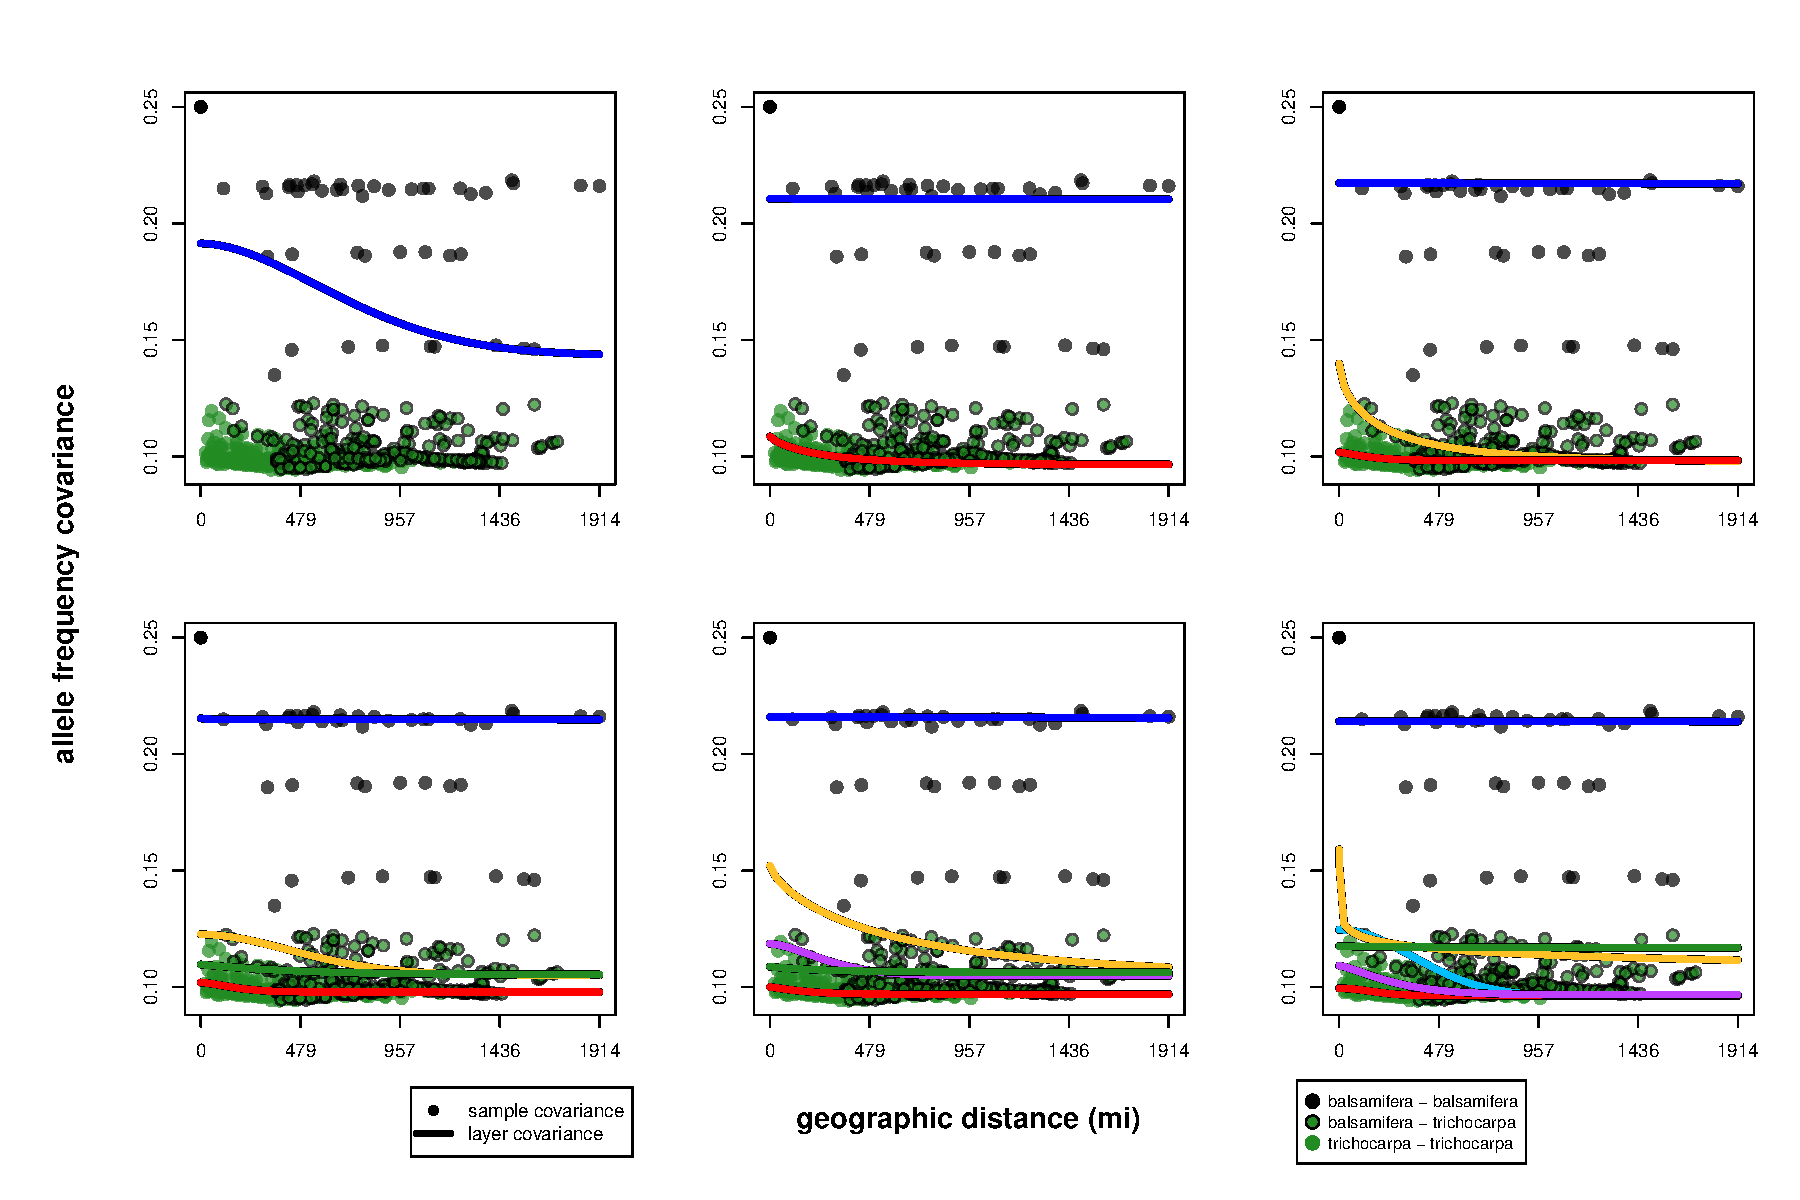
\includegraphics[width=\textwidth]{figs/populus/populus_sp_layer_covs.pdf}}
	\caption{
	Plots showing the layer-specific parametric covariance curves
	estimated for the \textit{Populus} data using 
	the spatial \texttt{conStruct} model run with $K=1$ through 6.
	Line colors are consistent with layer colors in Fig \ref{populus_sp_pies}.
	Points are colored by the species they are a covariance between:
	black on black points are sample covariances between populations of \textit{Populus balsamifera};
	green on black points are sample covariances between \bals{} and \tri{};
	green on green points are sample covariances between \tri{} and \tri{}.
    }\label{populus_sp_layer_covs}
\end{figure}
\clearpage

\begin{figure}
	\centering
		{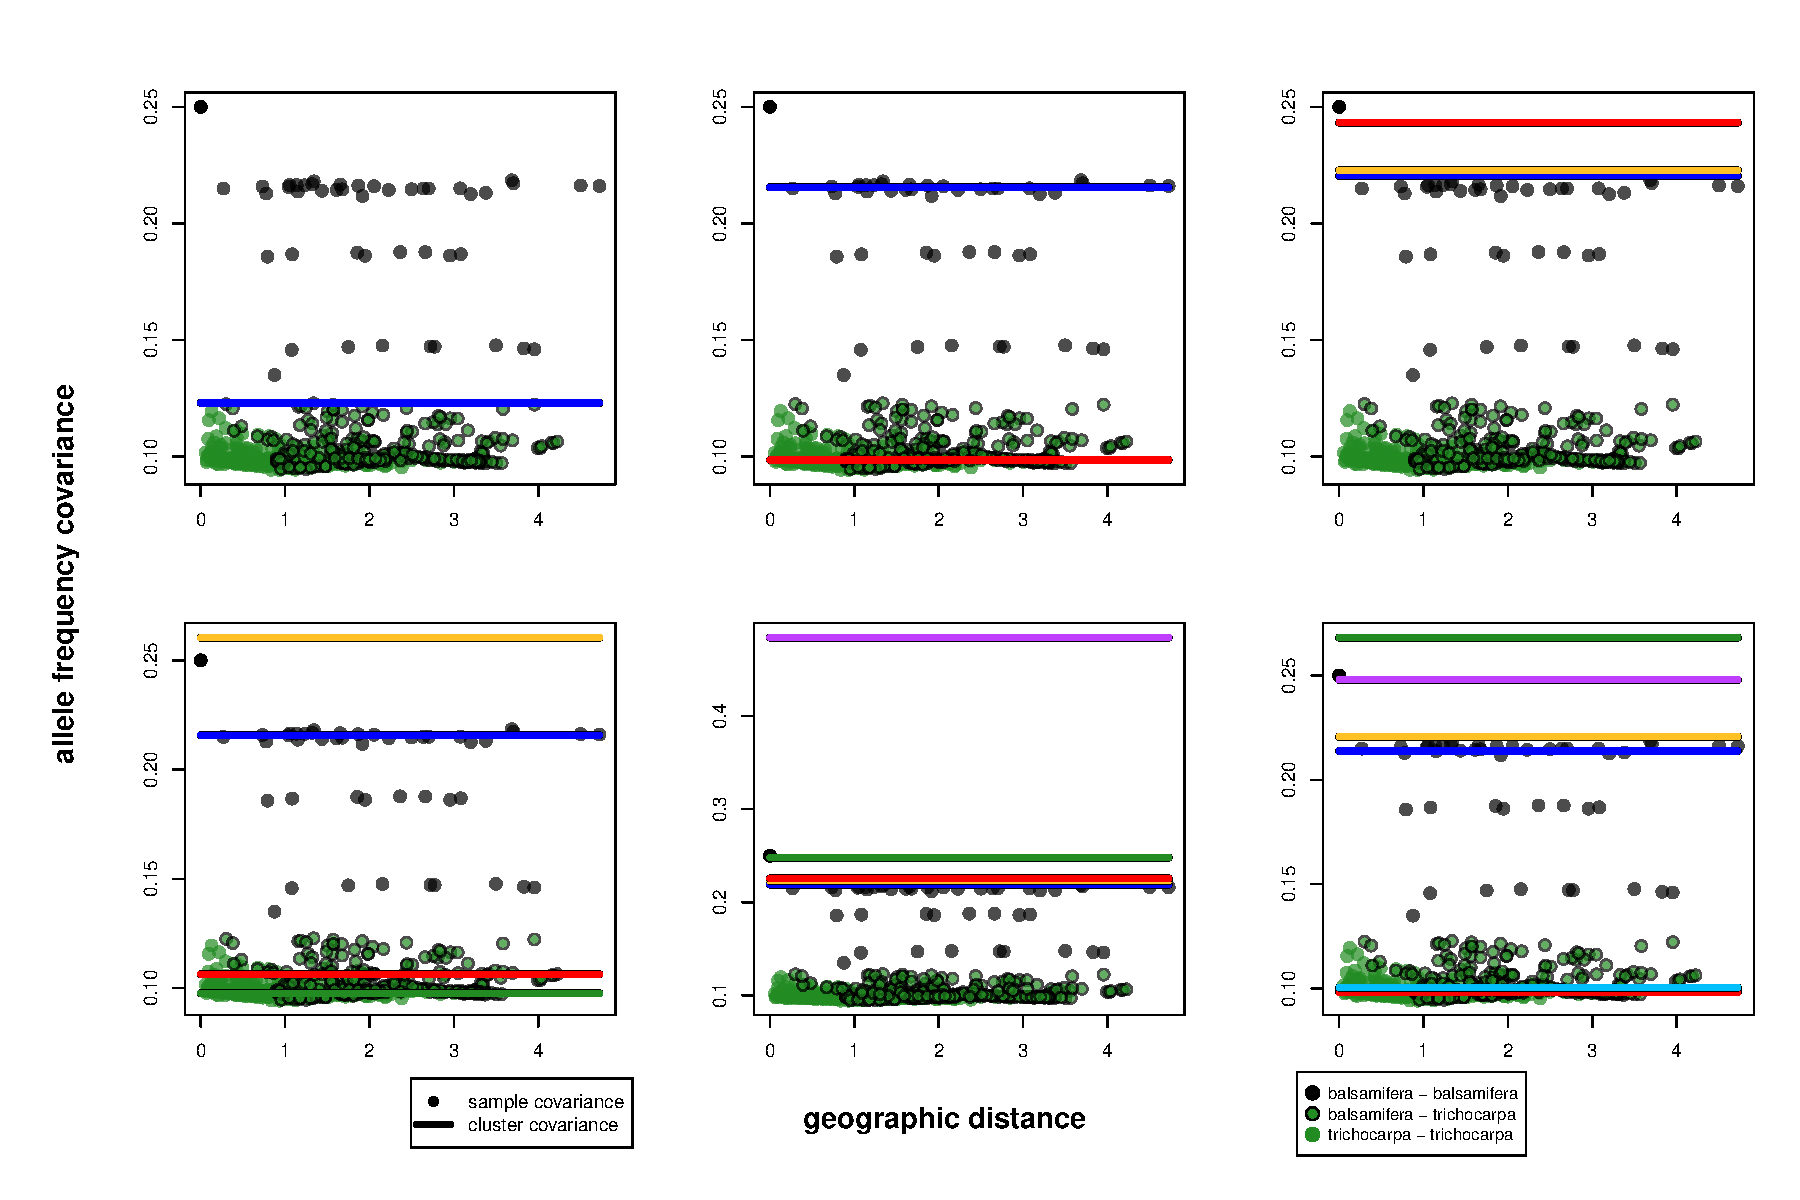
\includegraphics[width=\textwidth]{figs/populus/populus_nsp_layer_covs.pdf}}
	\caption{
	Plots showing the cluster-specific parametric covariances 
	estimated for the \textit{Populus} data using 
	the nonspatial \texttt{conStruct} model run with $K=1$ through 6.
	Line colors are consistent with cluster colors in Fig \ref{populus_nsp_pies}.
	Points are colored by the species they are a covariance between:
	black on black points are sample covariances between populations of \textit{Populus balsamifera};
	green on black points are sample covariances between \bals{} and \tri{};
	green on green points are sample covariances between \tri{} and \tri{}.
    }\label{populus_nsp_layer_covs}
\end{figure}
\clearpage

\begin{figure}
	\centering
		{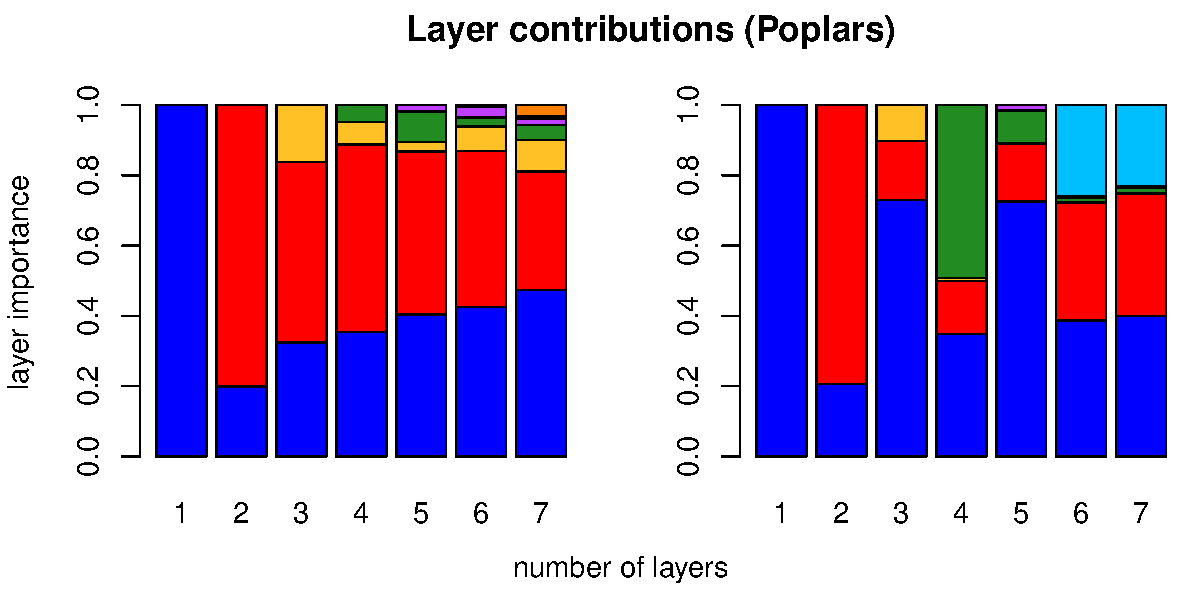
\includegraphics[width=\textwidth]{figs/populus/populus_laycon_barplots.pdf}}
	\caption{
	Layer/cluster contributions (i.e., how much total covariance is contributed by each layer/cluster), 
	for all layers estimated in runs using $K = 1$ through 7 
	for the spatial model (left), 
	and for all clusters using the nonspatial model (right).
	For each value of $K$ along the x-axis, there are an equal number of contributions plotted.
	Colors are consistent with Figs \ref{populus_sp_pies}, \ref{populus_sp_layer_covs}, \ref{populus_nsp_pies}, and \ref{populus_nsp_layer_covs}.
    }\label{populus_laycon}
\end{figure}
\clearpage

\begin{figure}
	\centering
		{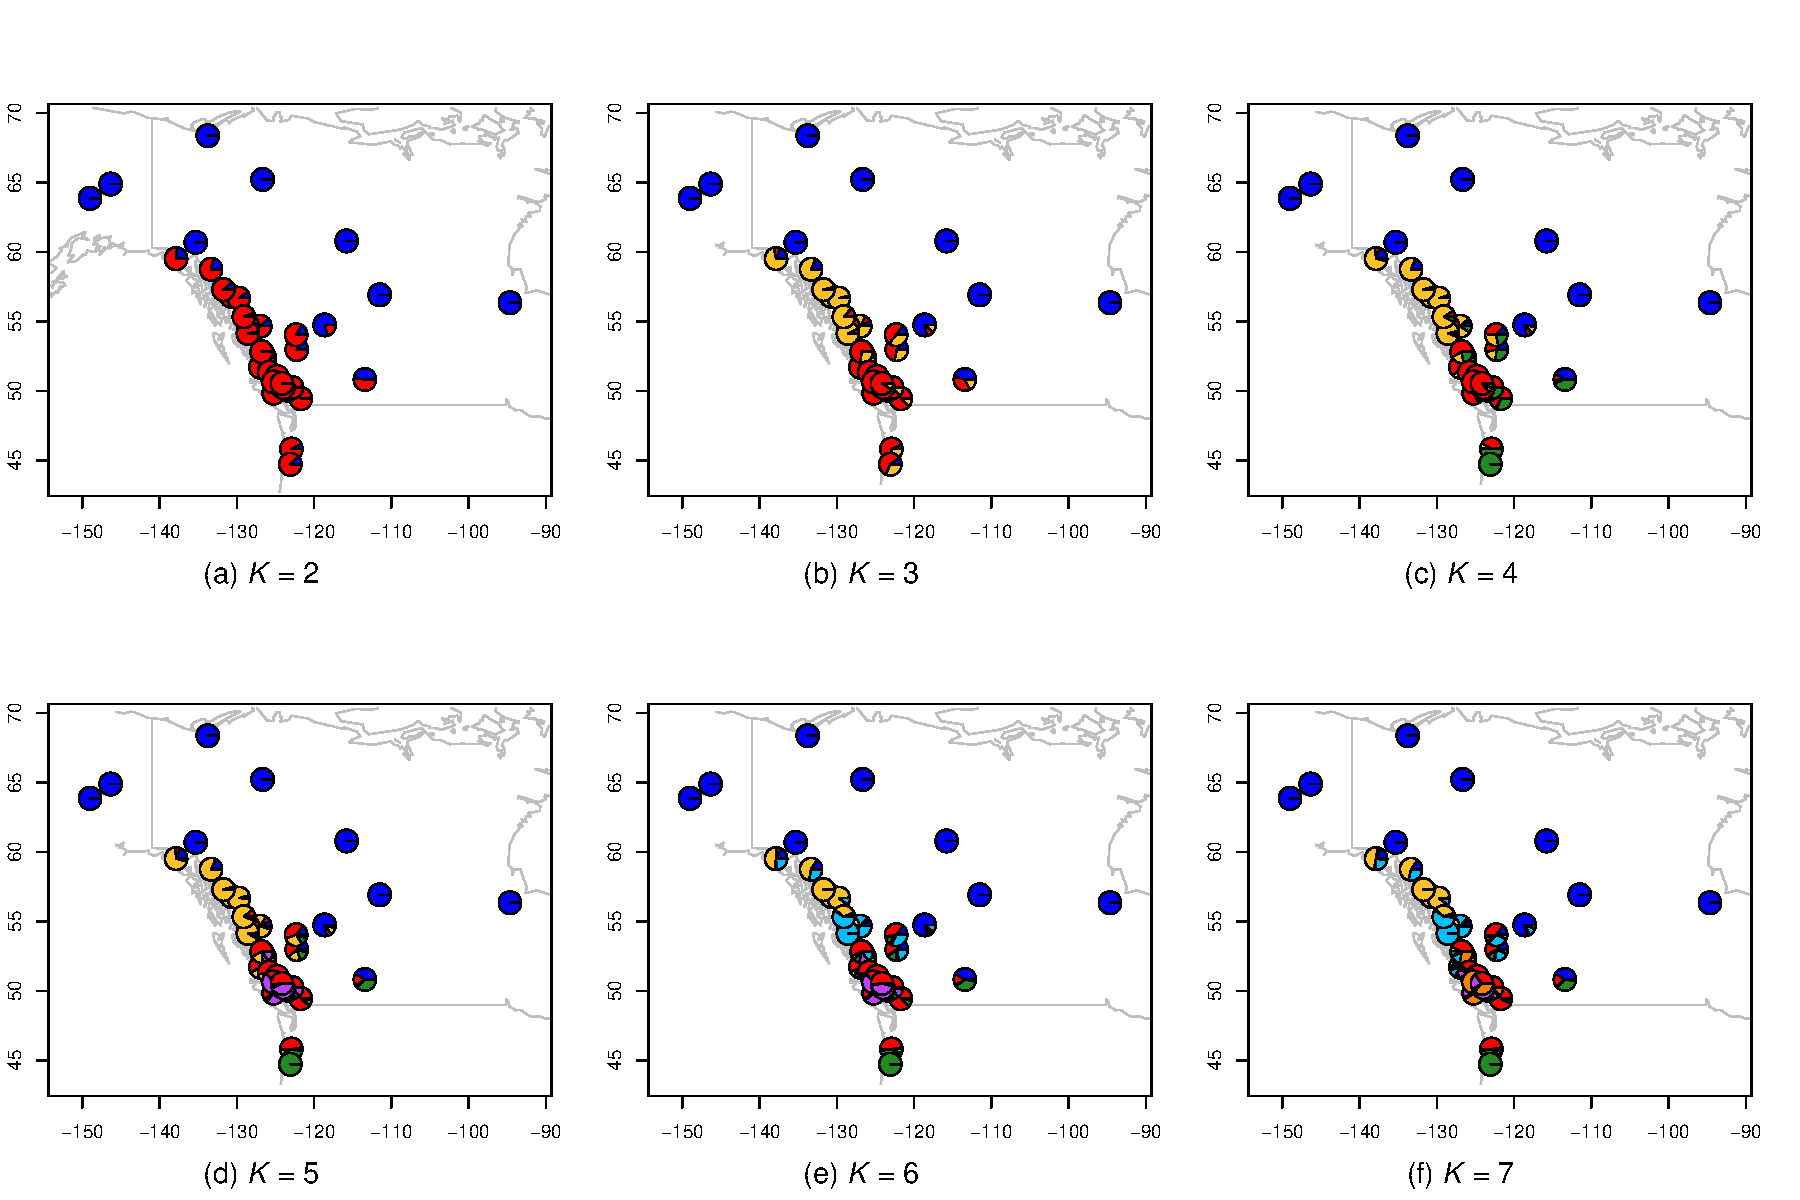
\includegraphics[width=\textwidth]{figs/populus/poplar_admixture_results.pdf}}
	\caption{
	Maps of admixture proportions estimated for the \textit{Populus} dataset 
	using ADMIXTURE \cite{ADMIXTURE} for $K=2$ through 7.
    }\label{populus_admixture}
\end{figure}
\clearpage

\begin{figure}
	\centering
		{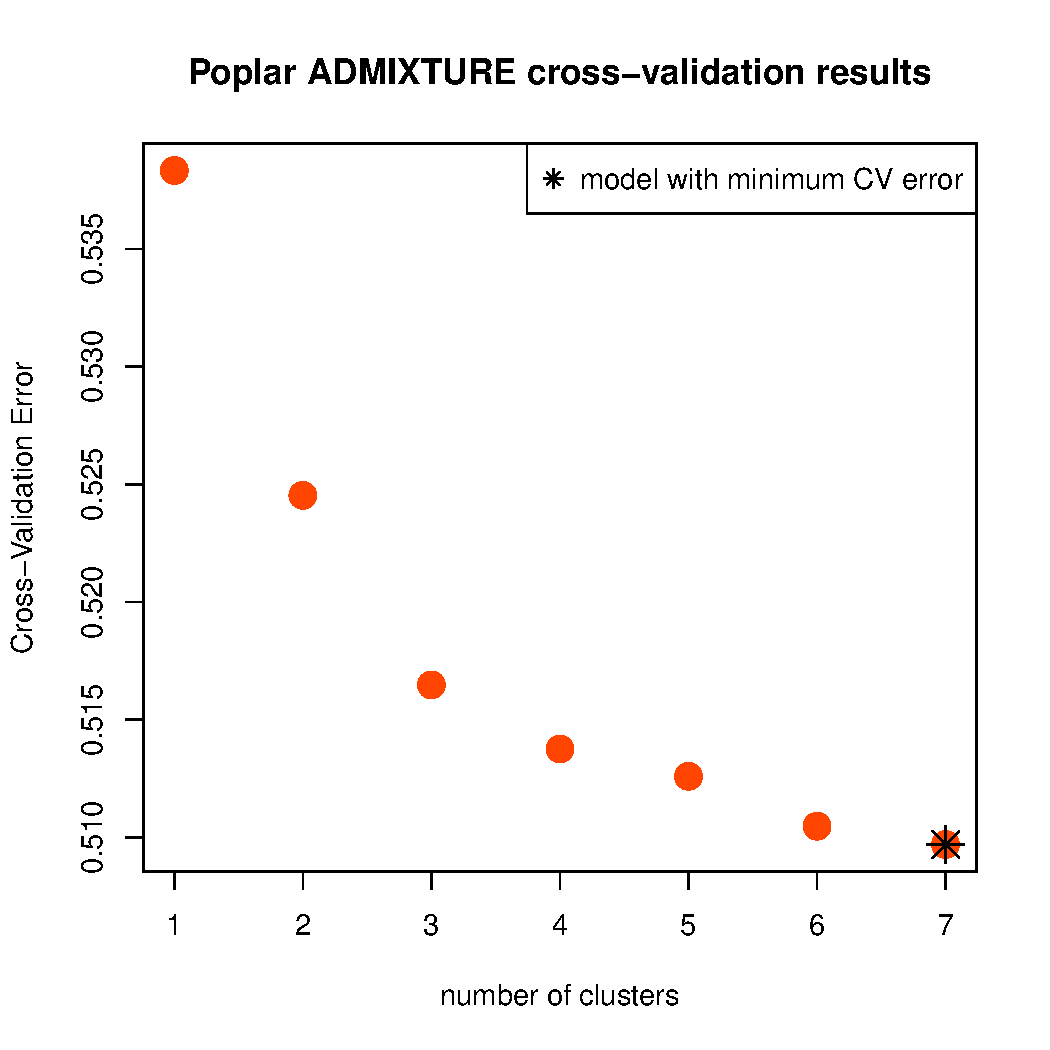
\includegraphics[width=\textwidth]{figs/populus/poplars_admixture_CVerror.pdf}}
	\caption{
	ADMIXTURE cross-validation results for poplar data, 
	run with $K=1$ through 7 using 50 data ``folds" (\texttt{--cv=50}).  
	The preferred model (with the lowest cross-validation error) is highlighted with an asterisk.
    }\label{poplar_admix_CVerrors}
\end{figure}
\clearpage

\begin{figure}
	\centering
		{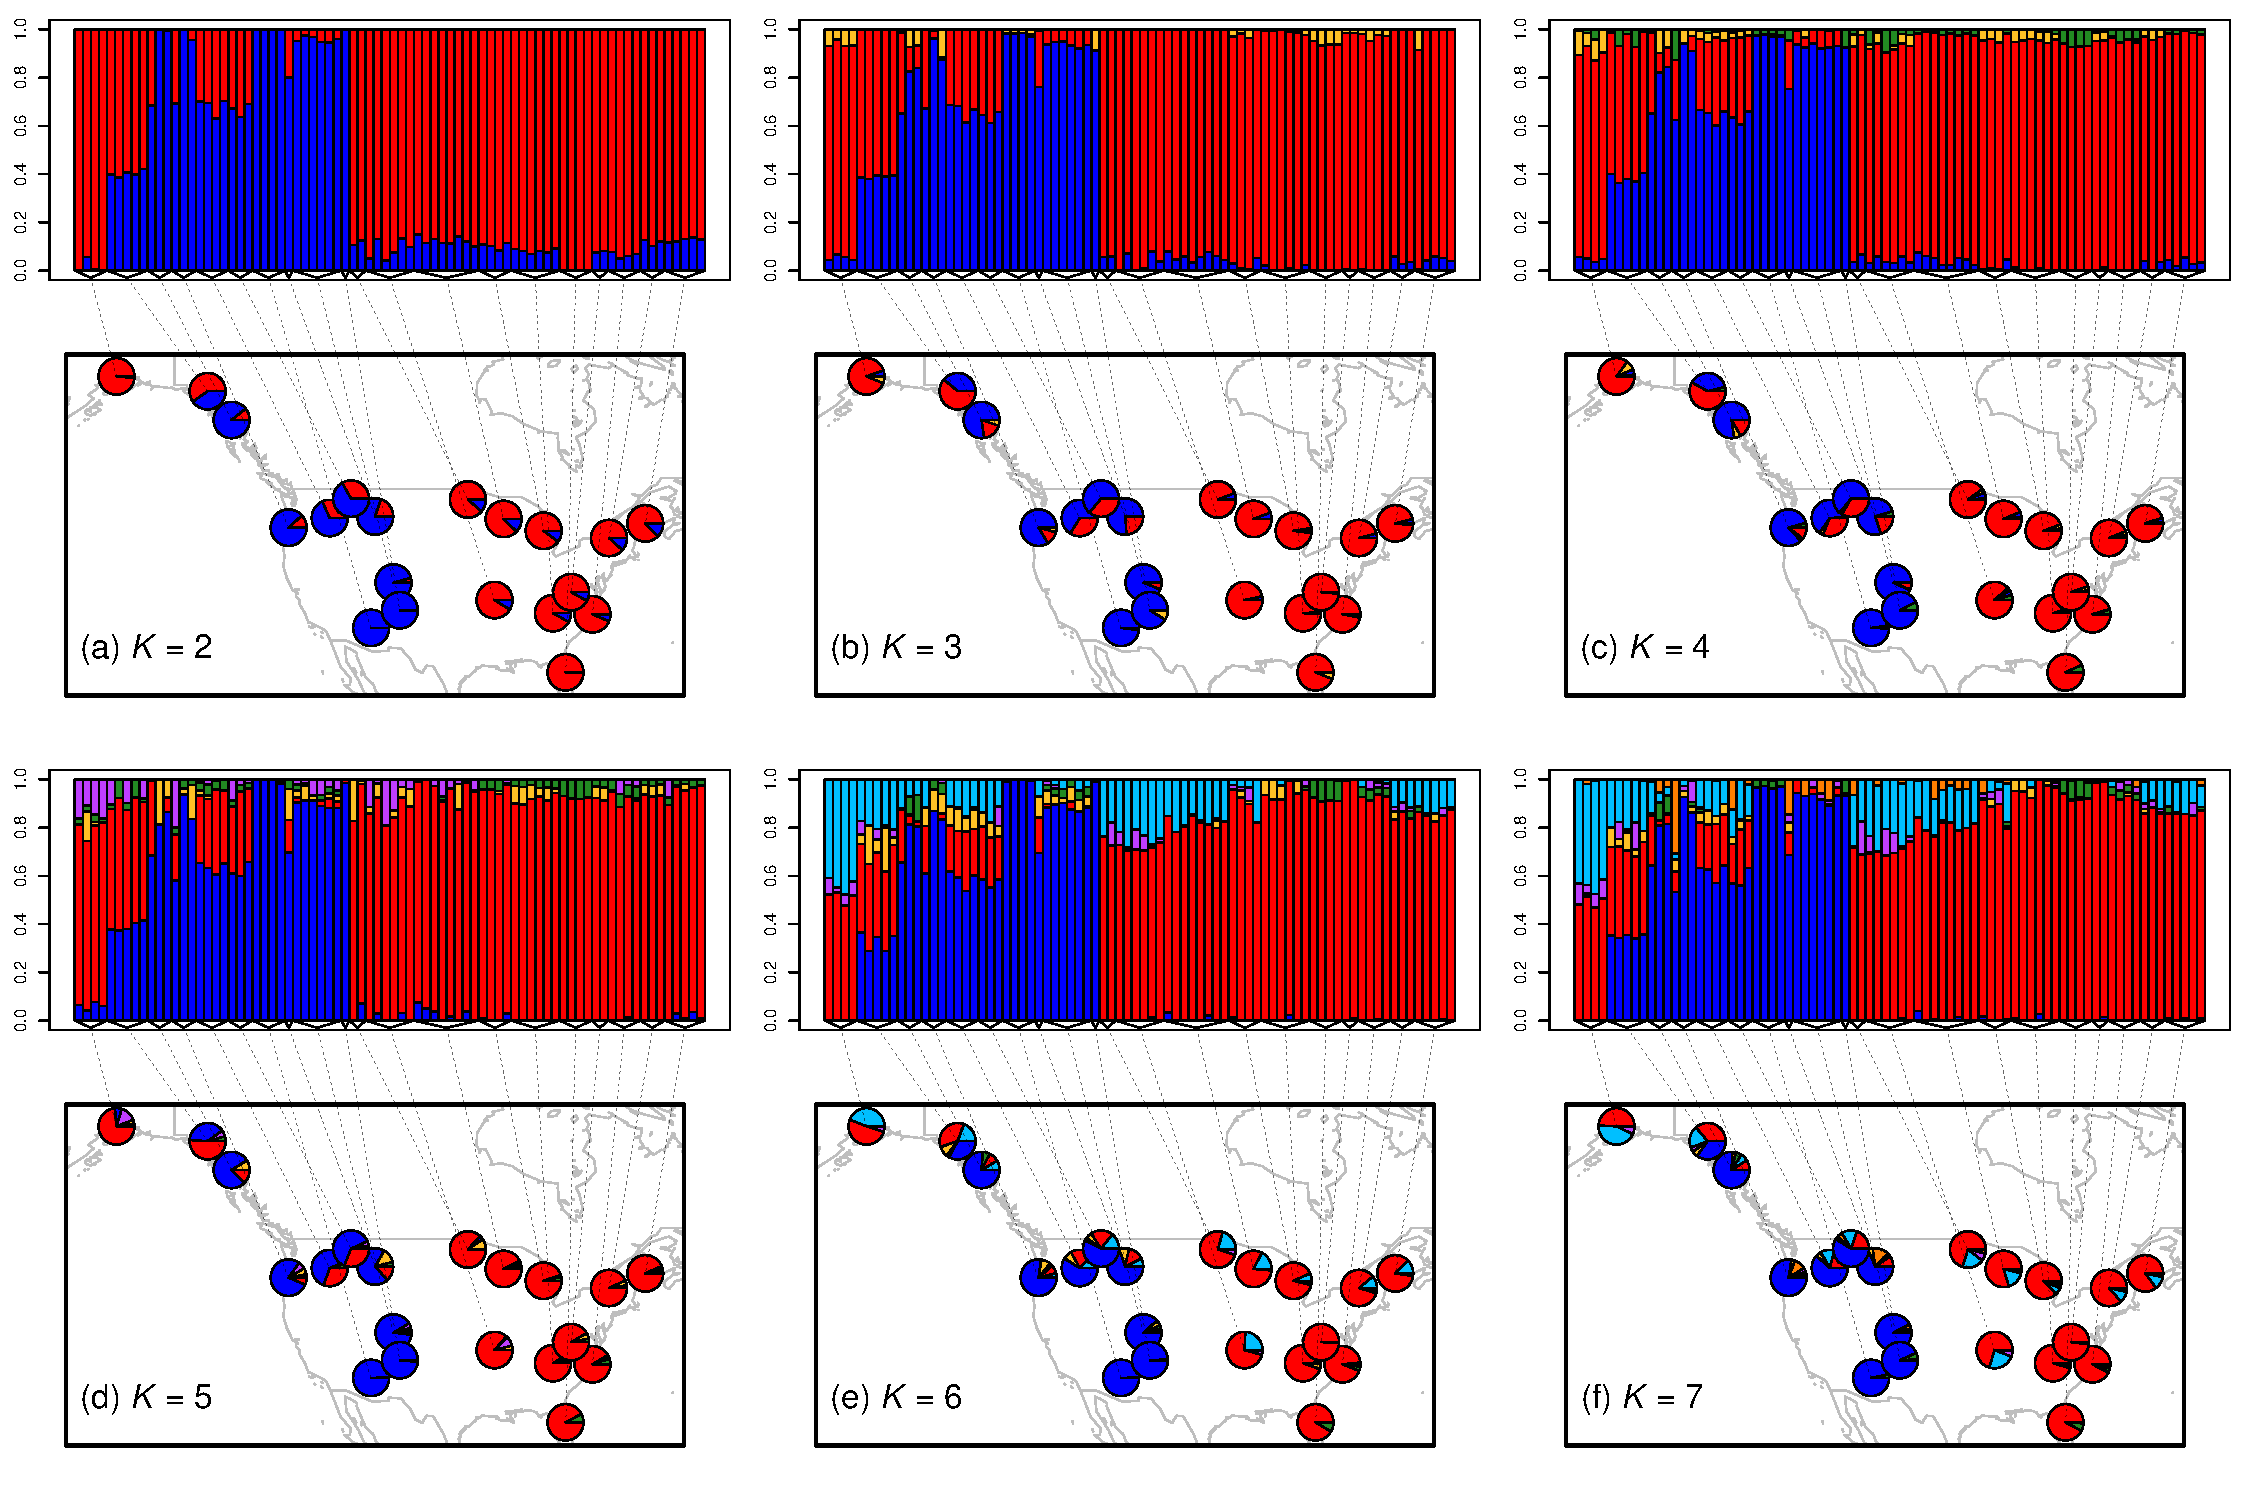
\includegraphics[width=\textwidth]{figs/bears/bear_sp_results.pdf}}
	\caption{
	Map of admixture proportions estimated for the bear dataset 
	using the spatial model for $K=2$ through 7.
    }\label{bear_sp_pies}
\end{figure}
\clearpage

\begin{figure}
	\centering
		{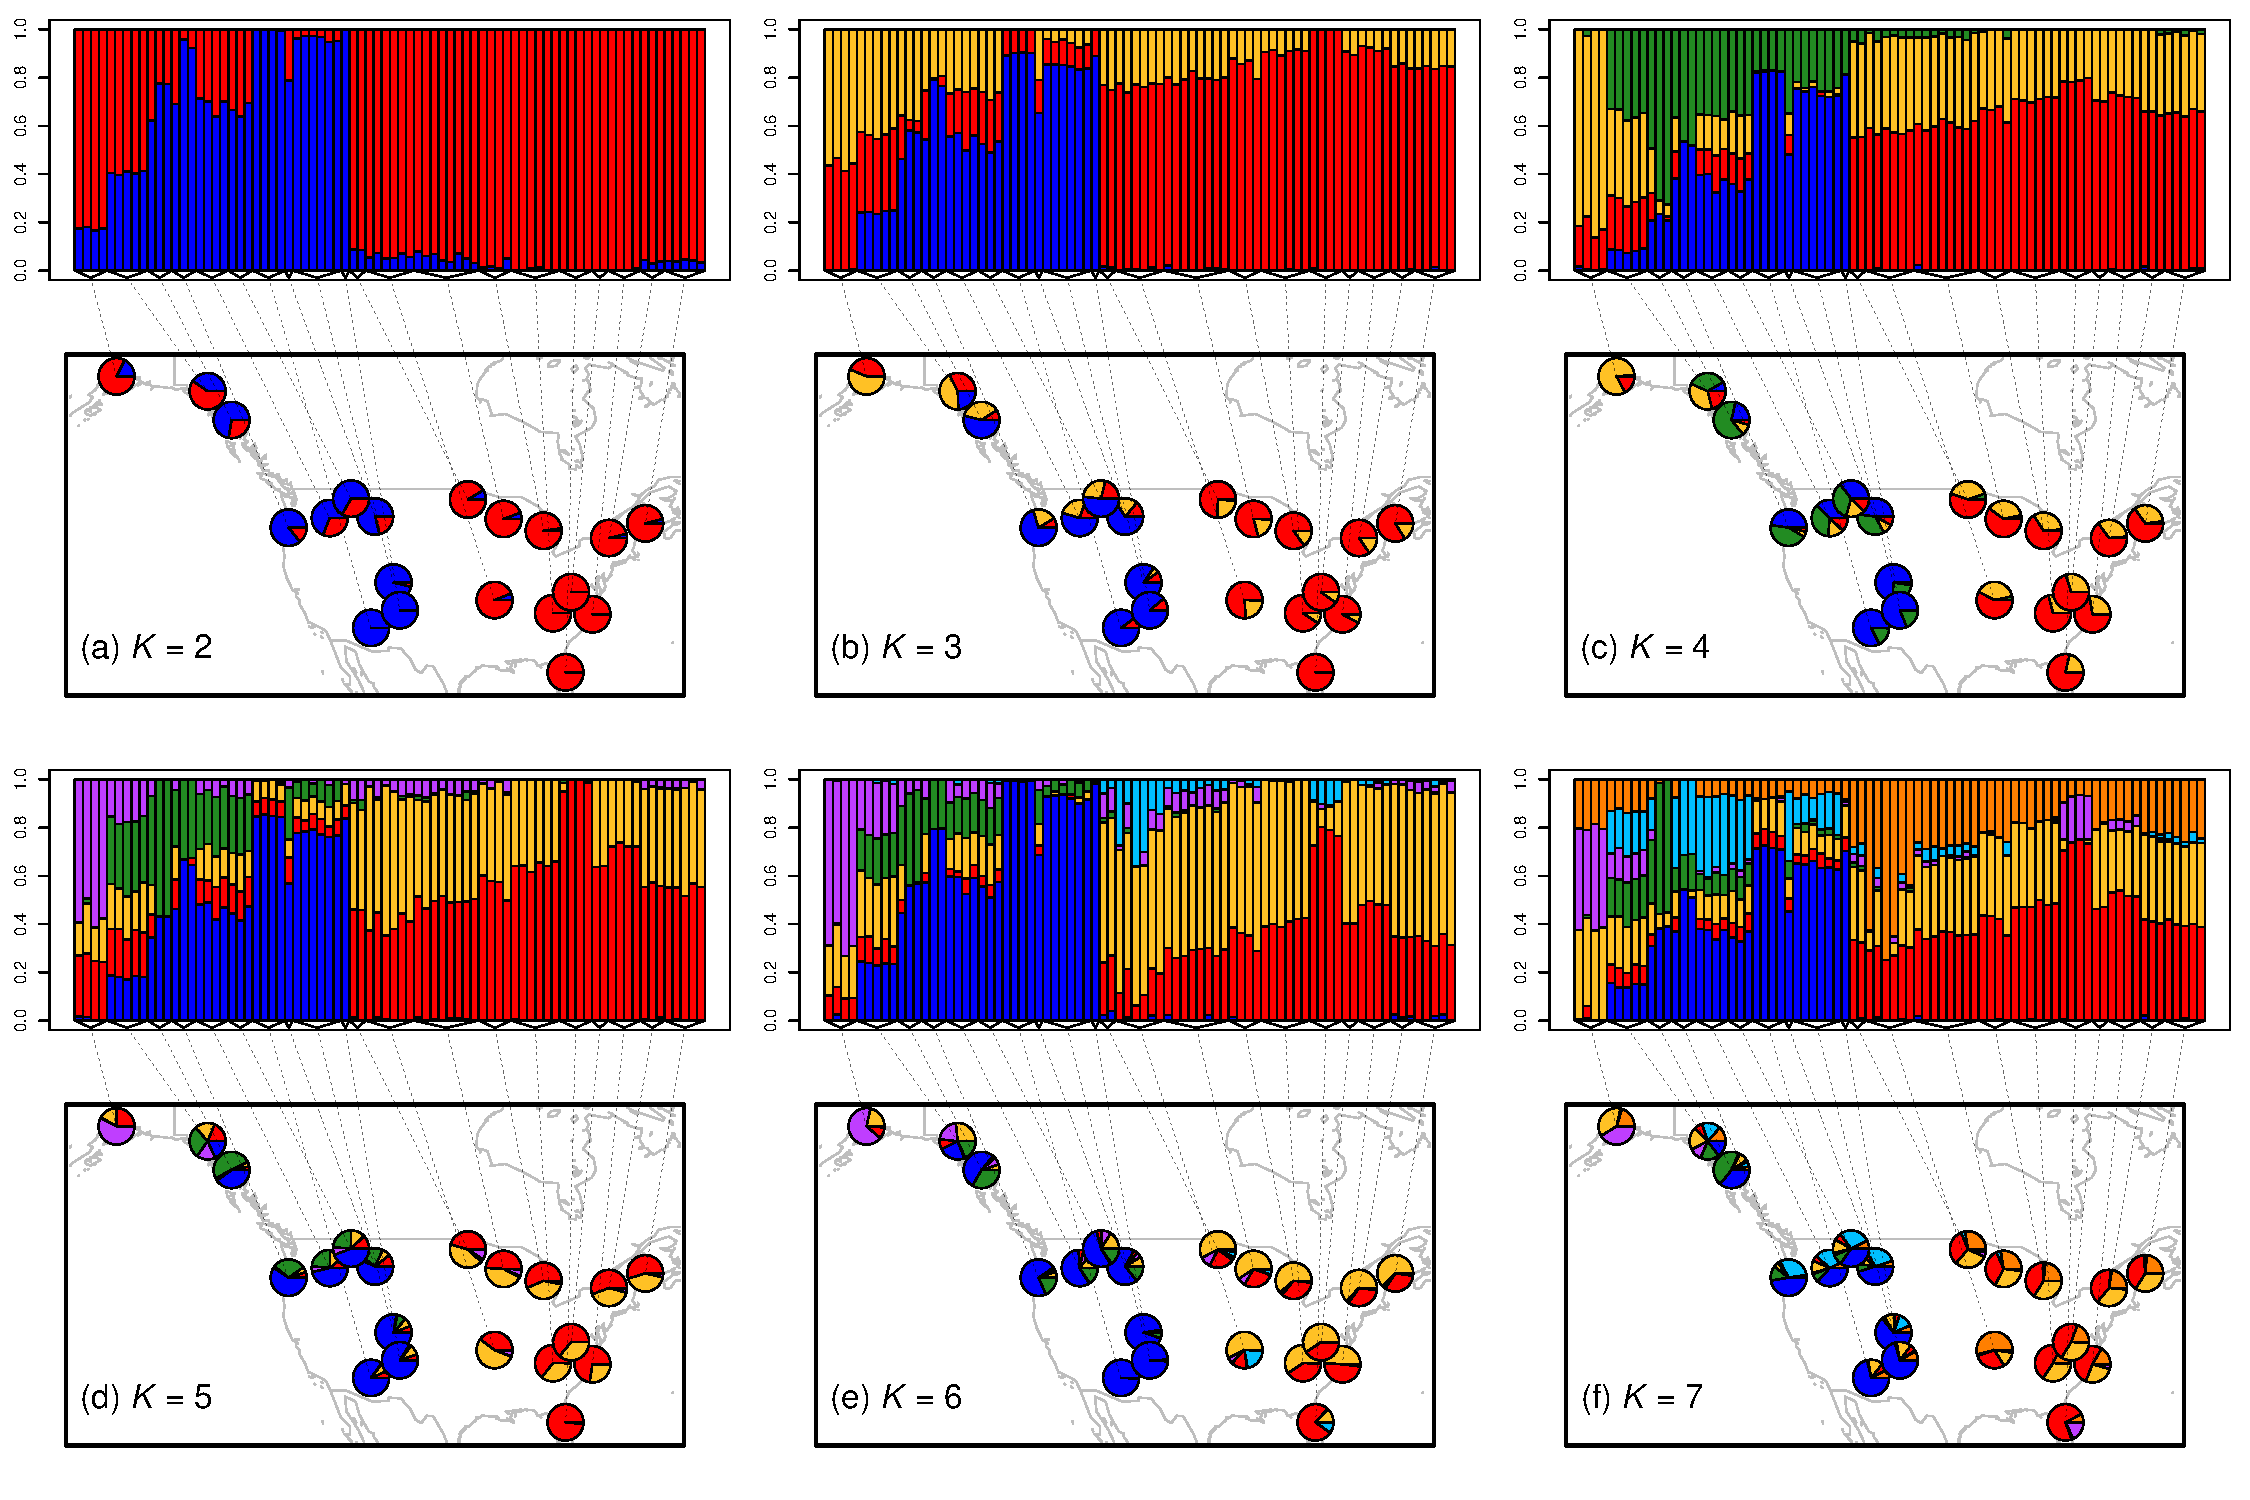
\includegraphics[width=\textwidth]{figs/bears/bear_nsp_results.pdf}}
	\caption{
	Map of admixture proportions estimated for the bear dataset 
	using the nonspatial model for $K=2$ through 7.
    }\label{bear_nsp_pies}
\end{figure}
\clearpage

\begin{figure}
	\centering
		{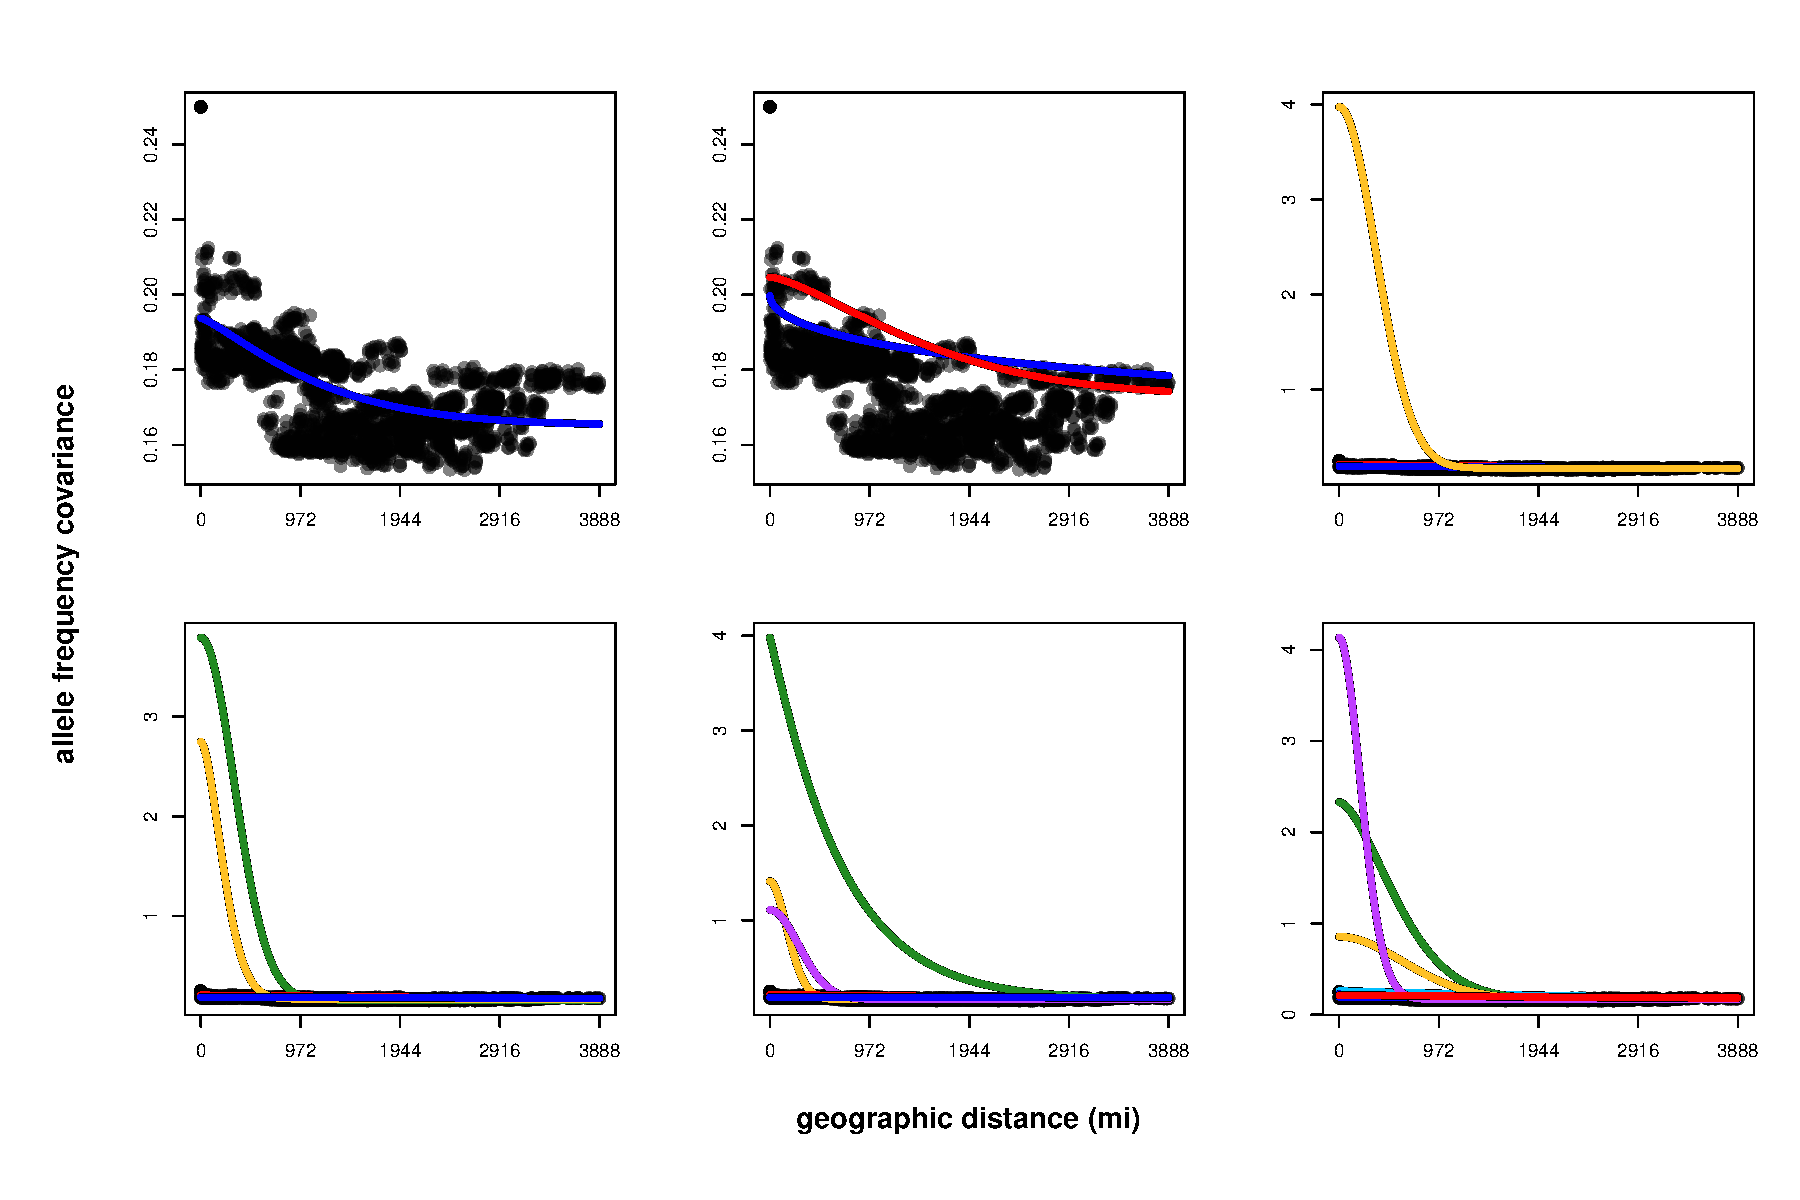
\includegraphics[width=\textwidth]{figs/bears/bear_sp_layer_covs.pdf}}
	\caption{
	Plots showing the layer-specific parametric covariance curves 
	estimated for the black bear data using 
	the spatial \texttt{conStruct} model run with $K=1$ through 6.
	 }\label{bear_sp_layer_covs}
\end{figure}
\clearpage

\begin{figure}
	\centering
		{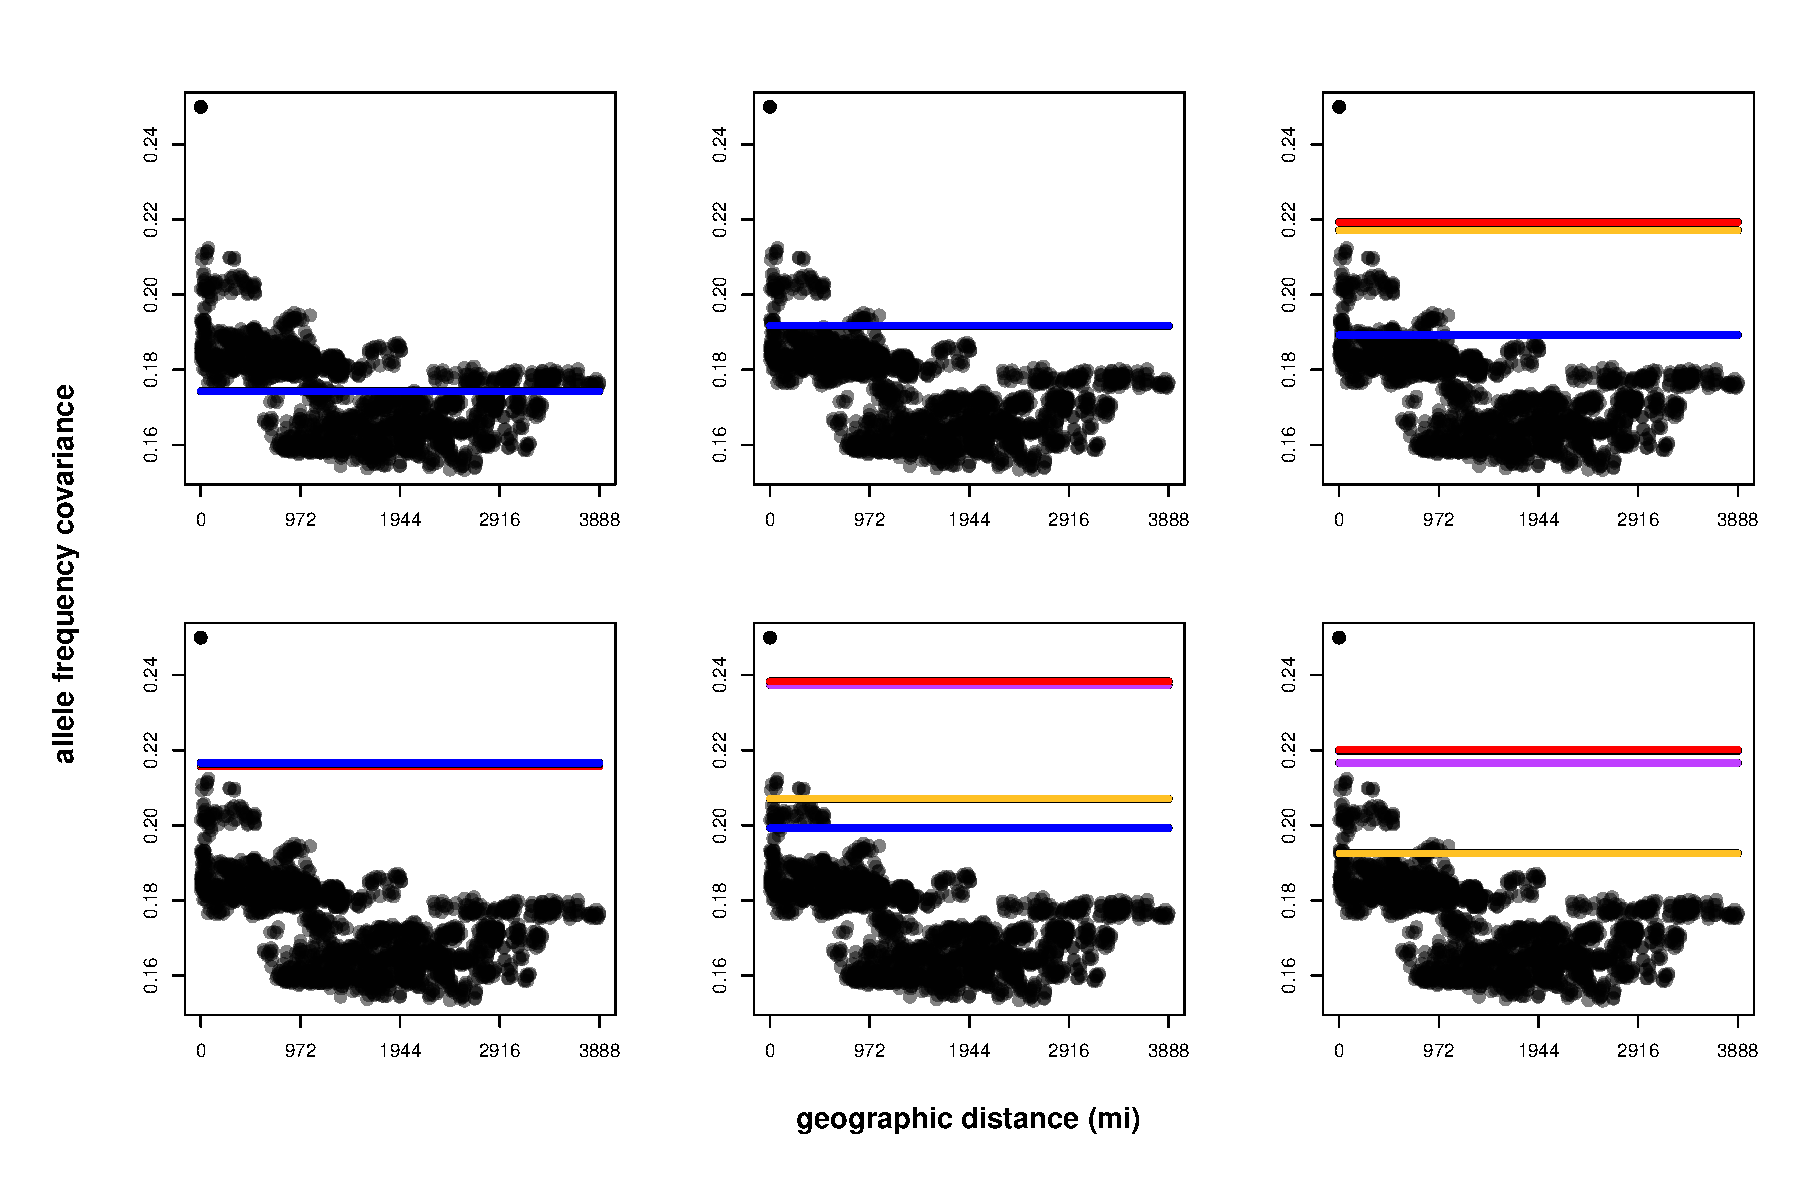
\includegraphics[width=\textwidth]{figs/bears/bear_nsp_layer_covs.pdf}}
	\caption{
	Plots showing the cluster-specific parametric covariances 
	estimated for the black bear data using 
	the nonspatial \texttt{conStruct} model run with $K=1$ through 6.
    }\label{bear_nsp_layer_covs}
\end{figure}
\clearpage

\begin{figure}
	\centering
		{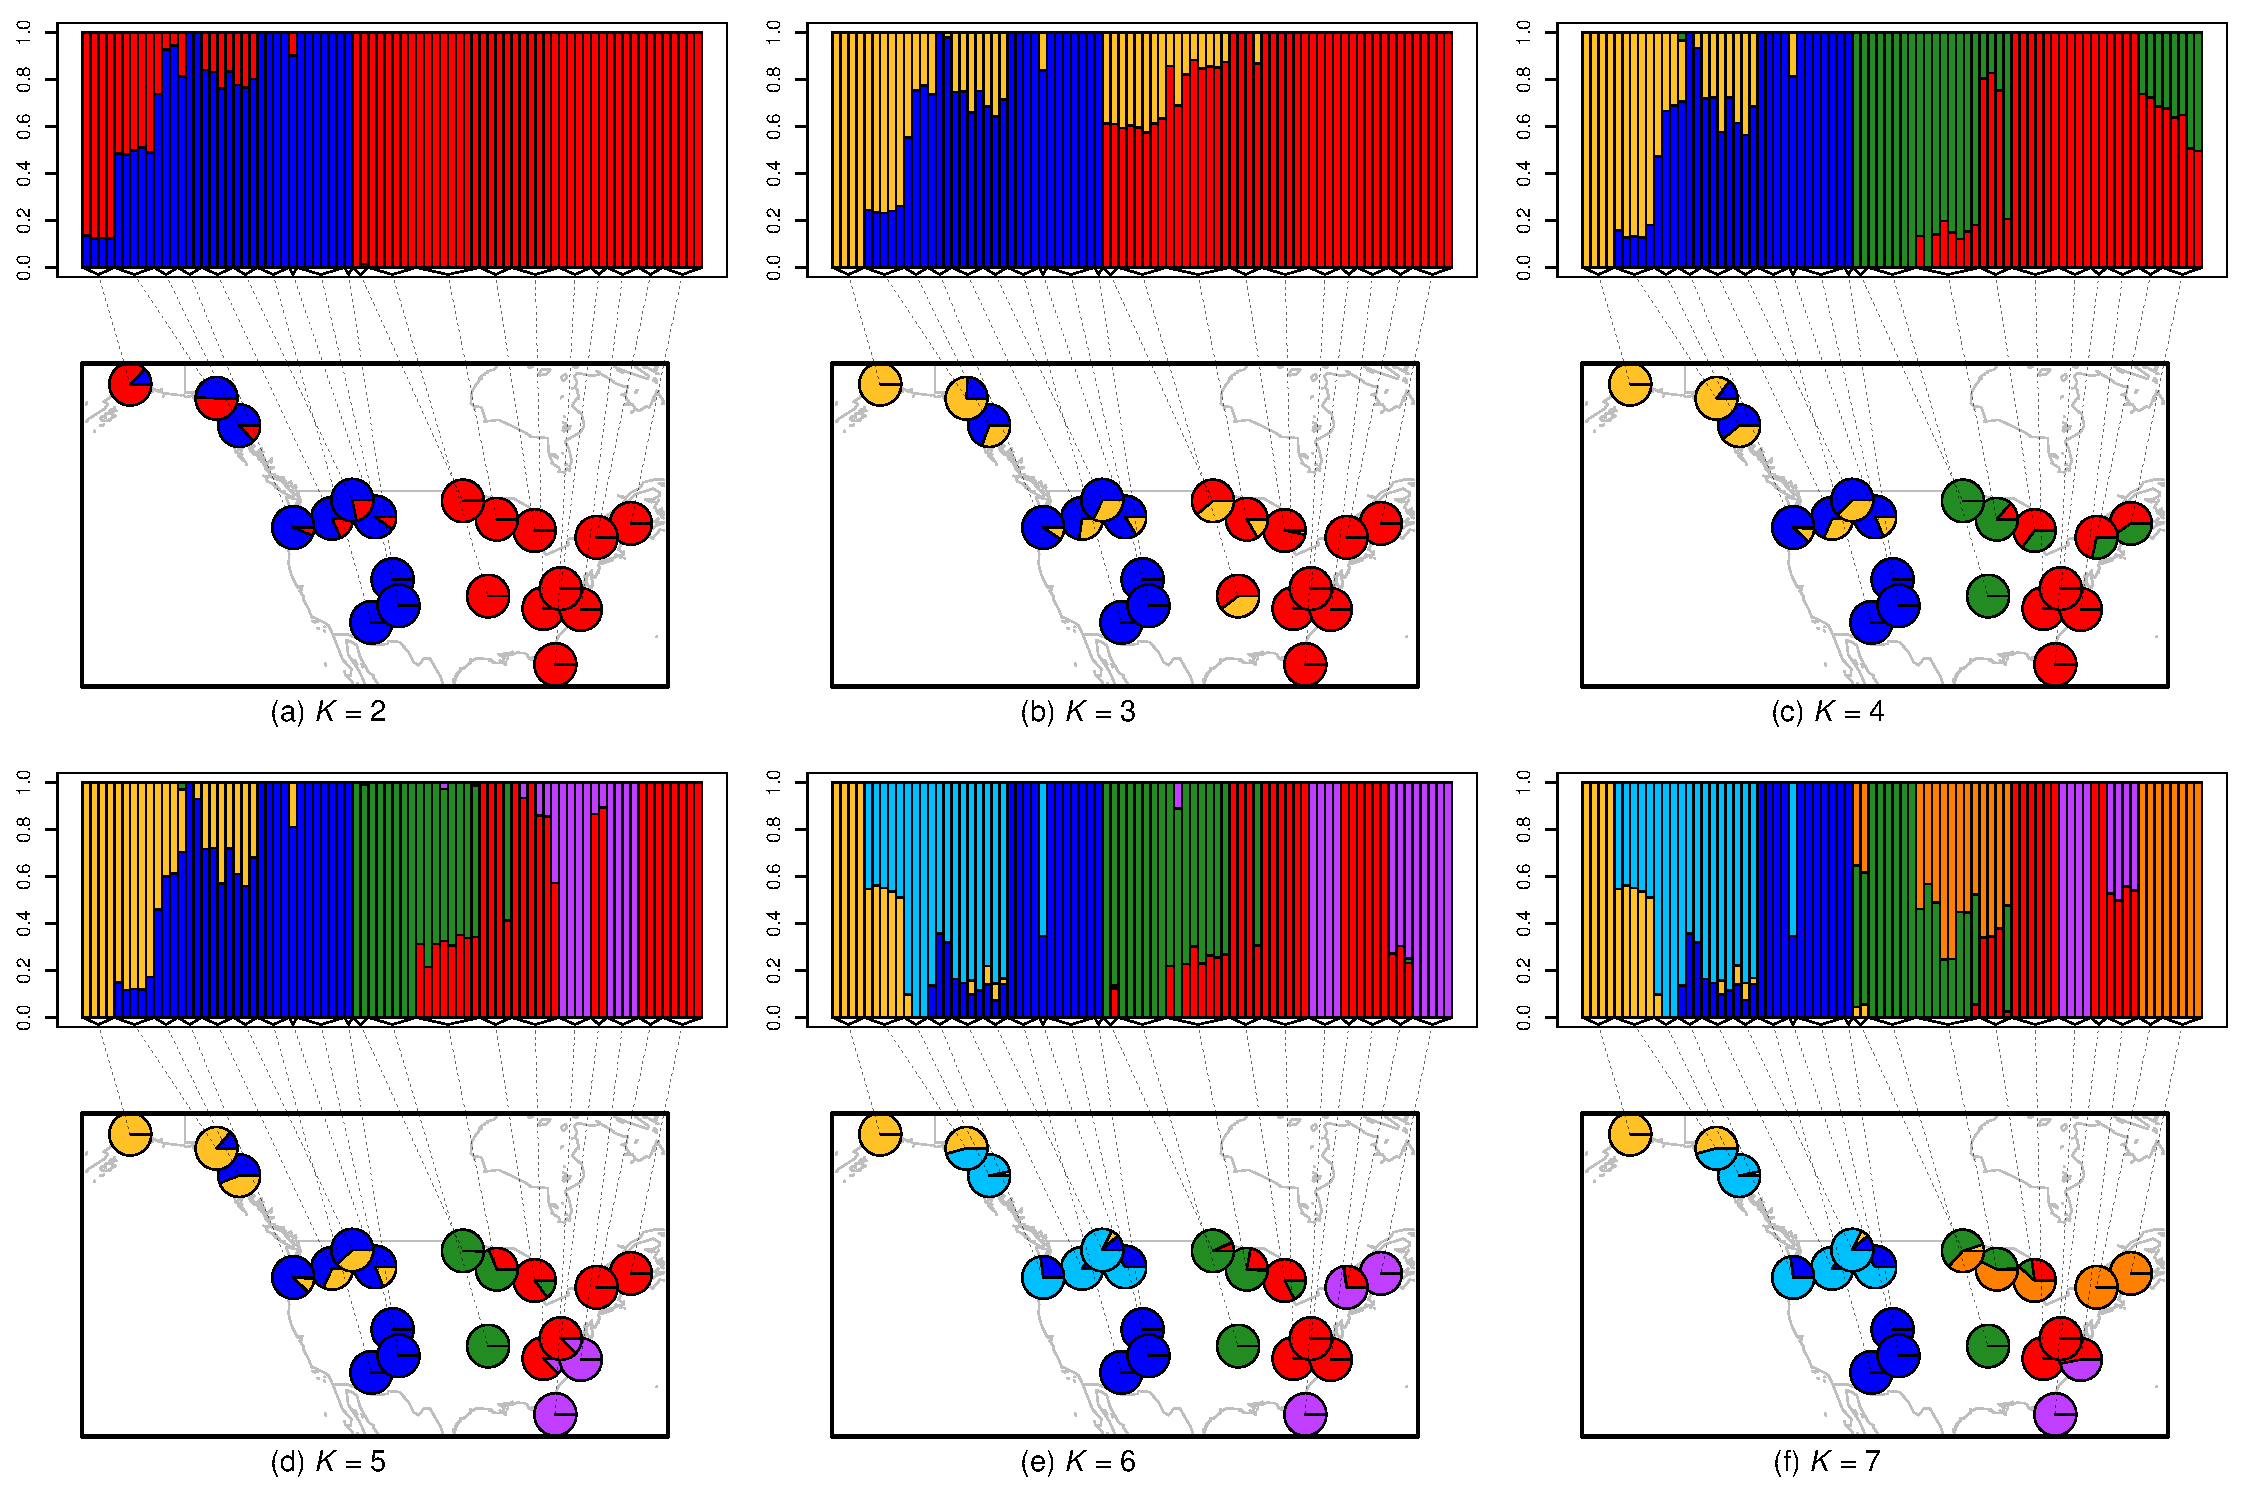
\includegraphics[width=\textwidth]{figs/bears/bear_admixture_results.pdf}}
	\caption{
	Maps of admixture proportions estimated for the bear dataset 
	using ADMIXTURE \cite{ADMIXTURE} for $K=2$ through 7.
    }\label{bear_admixture}
\end{figure}
\clearpage

\begin{figure}
	\centering
		{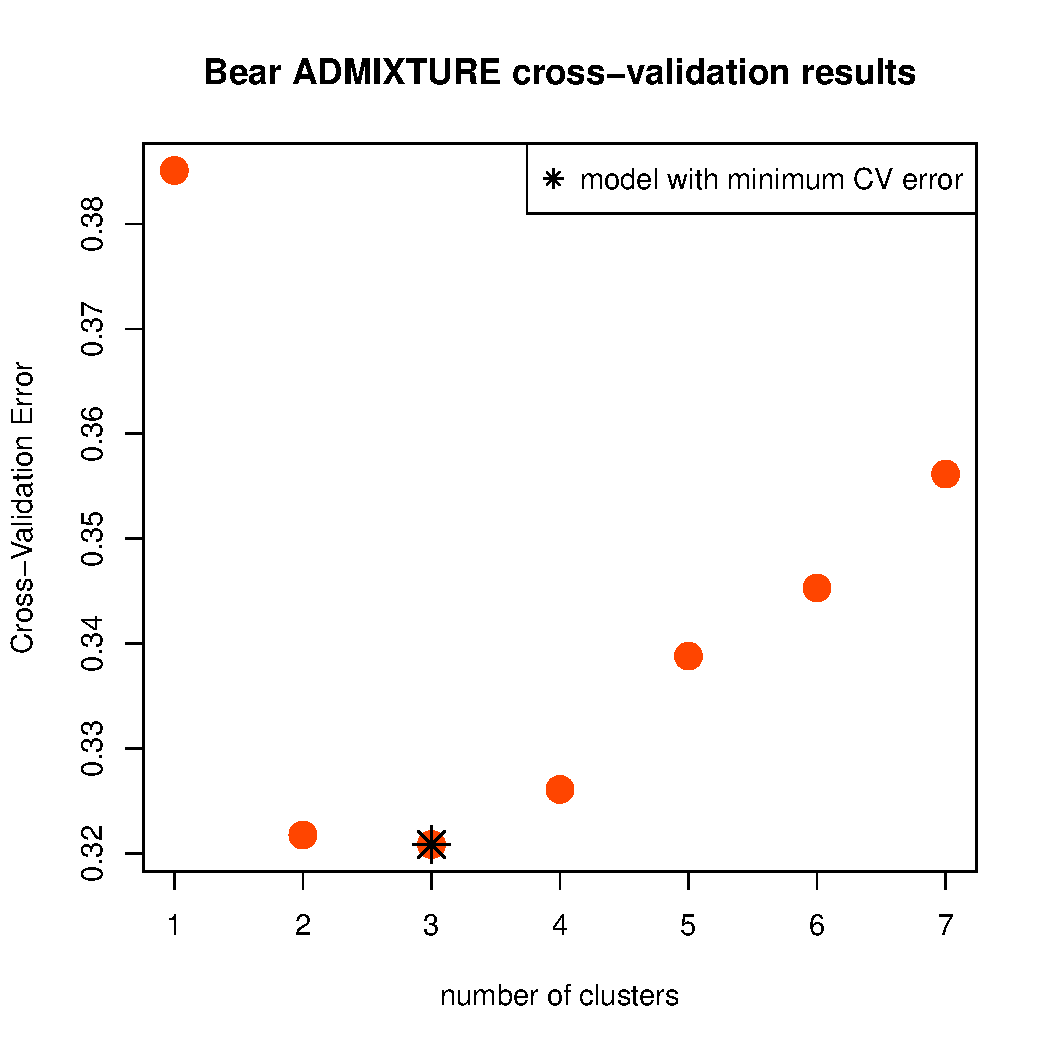
\includegraphics[width=\textwidth]{figs/bears/bear_admixture_CVerror.pdf}}
	\caption{
	ADMIXTURE cross-validation results for bear data, 
	run with $K=1$ through 7 using 50 data ``folds" (\texttt{--cv=50}).  
	The preferred model (with the lowest cross-validation error) is highlighted with an asterisk.
    }\label{bear_admix_CVerrors}
\end{figure}
\clearpage

%%% END IF INCLUDE SUPPLEMENT
\fi
\iffloatsatend
\renewcommand{\thetable}{\arabic{table}}
\setcounter{table}{0}
\renewcommand{\thefigure}{\arabic{figure}}
\setcounter{figure}{0}
\processdelayedfloats
\fi

\end{document}
